\documentclass[journal]{IEEEtran}
\usepackage[T1]{fontenc}
\usepackage{amsmath,amssymb}
\usepackage{graphicx,booktabs,array,multirow}
\usepackage{microtype}
\usepackage{xurl}
\usepackage[hidelinks]{hyperref}
\graphicspath{{figures/}}
\hyphenation{Earth-former crop-land Vid-arbha Mara-thwada Sen-ti-nel Conv-LSTM}
% generated by final_analyze.py from results_v2/final/rows.csv -- do not edit
\newcommand{\finNTestBlocks}{32}
\newcommand{\finNSuperblocks}{17}
\newcommand{\finNUnitsCore}{1{,}137}
\newcommand{\finNUnitsAllModels}{1{,}137}
\newcommand{\finNPixelForecasts}{50{,}144{,}593}
\newcommand{\finNTrainRows}{1{,}420{,}026}
\newcommand{\finNValRows}{89{,}907}
\newcommand{\finPersMAE}{0.0525}
\newcommand{\finPersRMSE}{0.0787}
\newcommand{\finPersBias}{0.0412}
\newcommand{\finPersPin}{0.0262}
\newcommand{\finPersCov}{--}
\newcommand{\finPersBelow}{--}
\newcommand{\finPersFallback}{0.0000}
\newcommand{\finPersRelMAE}{1.0000}
\newcommand{\finPersMAELeadOne}{0.0337}
\newcommand{\finPersPinLeadOne}{0.0168}
\newcommand{\finPersMAELeadTwo}{0.0525}
\newcommand{\finPersPinLeadTwo}{0.0262}
\newcommand{\finPersMAELeadThree}{0.0669}
\newcommand{\finPersPinLeadThree}{0.0335}
\newcommand{\finPersMAEYrTwentyFour}{0.0555}
\newcommand{\finPersPinYrTwentyFour}{0.0277}
\newcommand{\finPersMAEYrTwentyFive}{0.0499}
\newcommand{\finPersPinYrTwentyFive}{0.0250}
\newcommand{\finPersMAEKonkan}{0.0305}
\newcommand{\finPersMAEMarathwada}{0.0592}
\newcommand{\finPersMAENashik}{0.0579}
\newcommand{\finPersMAEPune}{0.0531}
\newcommand{\finPersMAEVidarbha}{0.0485}
\newcommand{\finPersMAEClearLow}{0.0666}
\newcommand{\finPersMAECropLow}{0.0440}
\newcommand{\finPersMAEClearMid}{0.0515}
\newcommand{\finPersMAECropMid}{0.0519}
\newcommand{\finPersMAEClearHigh}{0.0440}
\newcommand{\finPersMAECropHigh}{0.0584}
\newcommand{\finPersNGMAE}{0.0525}
\newcommand{\finPersNGRMSE}{0.0787}
\newcommand{\finPersNGBias}{0.0409}
\newcommand{\finPersNGPin}{0.0262}
\newcommand{\finPersNGCov}{--}
\newcommand{\finPersNGBelow}{--}
\newcommand{\finPersNGFallback}{0.5363}
\newcommand{\finPersNGRelMAE}{0.9996}
\newcommand{\finPersNGMAELeadOne}{0.0338}
\newcommand{\finPersNGPinLeadOne}{0.0169}
\newcommand{\finPersNGMAELeadTwo}{0.0525}
\newcommand{\finPersNGPinLeadTwo}{0.0262}
\newcommand{\finPersNGMAELeadThree}{0.0668}
\newcommand{\finPersNGPinLeadThree}{0.0334}
\newcommand{\finPersNGMAEYrTwentyFour}{0.0555}
\newcommand{\finPersNGPinYrTwentyFour}{0.0277}
\newcommand{\finPersNGMAEYrTwentyFive}{0.0498}
\newcommand{\finPersNGPinYrTwentyFive}{0.0249}
\newcommand{\finPersNGMAEKonkan}{0.0307}
\newcommand{\finPersNGMAEMarathwada}{0.0591}
\newcommand{\finPersNGMAENashik}{0.0579}
\newcommand{\finPersNGMAEPune}{0.0532}
\newcommand{\finPersNGMAEVidarbha}{0.0485}
\newcommand{\finPersNGMAEClearLow}{0.0664}
\newcommand{\finPersNGMAECropLow}{0.0441}
\newcommand{\finPersNGMAEClearMid}{0.0515}
\newcommand{\finPersNGMAECropMid}{0.0519}
\newcommand{\finPersNGMAEClearHigh}{0.0441}
\newcommand{\finPersNGMAECropHigh}{0.0584}
\newcommand{\finMovAvgMAE}{0.0866}
\newcommand{\finMovAvgRMSE}{0.1073}
\newcommand{\finMovAvgBias}{0.0837}
\newcommand{\finMovAvgPin}{0.0433}
\newcommand{\finMovAvgCov}{--}
\newcommand{\finMovAvgBelow}{--}
\newcommand{\finMovAvgFallback}{0.0000}
\newcommand{\finMovAvgRelMAE}{1.6499}
\newcommand{\finMovAvgMAELeadOne}{0.0730}
\newcommand{\finMovAvgPinLeadOne}{0.0365}
\newcommand{\finMovAvgMAELeadTwo}{0.0875}
\newcommand{\finMovAvgPinLeadTwo}{0.0437}
\newcommand{\finMovAvgMAELeadThree}{0.0962}
\newcommand{\finMovAvgPinLeadThree}{0.0481}
\newcommand{\finMovAvgMAEYrTwentyFour}{0.0918}
\newcommand{\finMovAvgPinYrTwentyFour}{0.0459}
\newcommand{\finMovAvgMAEYrTwentyFive}{0.0820}
\newcommand{\finMovAvgPinYrTwentyFive}{0.0410}
\newcommand{\finMovAvgMAEKonkan}{0.0676}
\newcommand{\finMovAvgMAEMarathwada}{0.0902}
\newcommand{\finMovAvgMAENashik}{0.0954}
\newcommand{\finMovAvgMAEPune}{0.0876}
\newcommand{\finMovAvgMAEVidarbha}{0.0808}
\newcommand{\finMovAvgMAEClearLow}{0.0939}
\newcommand{\finMovAvgMAECropLow}{0.0775}
\newcommand{\finMovAvgMAEClearMid}{0.0860}
\newcommand{\finMovAvgMAECropMid}{0.0890}
\newcommand{\finMovAvgMAEClearHigh}{0.0823}
\newcommand{\finMovAvgMAECropHigh}{0.0899}
\newcommand{\finSeasMAE}{0.0476}
\newcommand{\finSeasRMSE}{0.0717}
\newcommand{\finSeasBias}{0.0275}
\newcommand{\finSeasPin}{0.0238}
\newcommand{\finSeasCov}{--}
\newcommand{\finSeasBelow}{--}
\newcommand{\finSeasFallback}{0.6419}
\newcommand{\finSeasRelMAE}{0.9072}
\newcommand{\finSeasMAELeadOne}{0.0345}
\newcommand{\finSeasPinLeadOne}{0.0172}
\newcommand{\finSeasMAELeadTwo}{0.0480}
\newcommand{\finSeasPinLeadTwo}{0.0240}
\newcommand{\finSeasMAELeadThree}{0.0574}
\newcommand{\finSeasPinLeadThree}{0.0287}
\newcommand{\finSeasMAEYrTwentyFour}{0.0514}
\newcommand{\finSeasPinYrTwentyFour}{0.0257}
\newcommand{\finSeasMAEYrTwentyFive}{0.0443}
\newcommand{\finSeasPinYrTwentyFive}{0.0222}
\newcommand{\finSeasMAEKonkan}{0.0300}
\newcommand{\finSeasMAEMarathwada}{0.0540}
\newcommand{\finSeasMAENashik}{0.0502}
\newcommand{\finSeasMAEPune}{0.0503}
\newcommand{\finSeasMAEVidarbha}{0.0439}
\newcommand{\finSeasMAEClearLow}{0.0570}
\newcommand{\finSeasMAECropLow}{0.0419}
\newcommand{\finSeasMAEClearMid}{0.0475}
\newcommand{\finSeasMAECropMid}{0.0467}
\newcommand{\finSeasMAEClearHigh}{0.0416}
\newcommand{\finSeasMAECropHigh}{0.0522}
\newcommand{\finClimMAE}{0.0307}
\newcommand{\finClimRMSE}{0.0425}
\newcommand{\finClimBias}{-0.0042}
\newcommand{\finClimPin}{0.0108}
\newcommand{\finClimCov}{0.5560}
\newcommand{\finClimBelow}{0.1625}
\newcommand{\finClimFallback}{0.4568}
\newcommand{\finClimRelMAE}{0.5841}
\newcommand{\finClimMAELeadOne}{0.0299}
\newcommand{\finClimPinLeadOne}{0.0104}
\newcommand{\finClimMAELeadTwo}{0.0304}
\newcommand{\finClimPinLeadTwo}{0.0106}
\newcommand{\finClimMAELeadThree}{0.0315}
\newcommand{\finClimPinLeadThree}{0.0111}
\newcommand{\finClimMAEYrTwentyFour}{0.0303}
\newcommand{\finClimPinYrTwentyFour}{0.0107}
\newcommand{\finClimMAEYrTwentyFive}{0.0309}
\newcommand{\finClimPinYrTwentyFive}{0.0108}
\newcommand{\finClimMAEKonkan}{0.0330}
\newcommand{\finClimMAEMarathwada}{0.0362}
\newcommand{\finClimMAENashik}{0.0270}
\newcommand{\finClimMAEPune}{0.0314}
\newcommand{\finClimMAEVidarbha}{0.0274}
\newcommand{\finClimMAEClearLow}{0.0286}
\newcommand{\finClimMAECropLow}{0.0304}
\newcommand{\finClimMAEClearMid}{0.0304}
\newcommand{\finClimMAECropMid}{0.0281}
\newcommand{\finClimMAEClearHigh}{0.0322}
\newcommand{\finClimMAECropHigh}{0.0335}
\newcommand{\finRidgeMAE}{0.0297}
\newcommand{\finRidgeRMSE}{0.0426}
\newcommand{\finRidgeBias}{0.0080}
\newcommand{\finRidgePin}{0.0148}
\newcommand{\finRidgeCov}{--}
\newcommand{\finRidgeBelow}{--}
\newcommand{\finRidgeFallback}{0.0000}
\newcommand{\finRidgeRelMAE}{0.5654}
\newcommand{\finRidgeMAELeadOne}{0.0268}
\newcommand{\finRidgePinLeadOne}{0.0134}
\newcommand{\finRidgeMAELeadTwo}{0.0299}
\newcommand{\finRidgePinLeadTwo}{0.0149}
\newcommand{\finRidgeMAELeadThree}{0.0317}
\newcommand{\finRidgePinLeadThree}{0.0159}
\newcommand{\finRidgeMAEYrTwentyFour}{0.0304}
\newcommand{\finRidgePinYrTwentyFour}{0.0152}
\newcommand{\finRidgeMAEYrTwentyFive}{0.0290}
\newcommand{\finRidgePinYrTwentyFive}{0.0145}
\newcommand{\finRidgeMAEKonkan}{0.0274}
\newcommand{\finRidgeMAEMarathwada}{0.0345}
\newcommand{\finRidgeMAENashik}{0.0299}
\newcommand{\finRidgeMAEPune}{0.0291}
\newcommand{\finRidgeMAEVidarbha}{0.0258}
\newcommand{\finRidgeMAEClearLow}{0.0309}
\newcommand{\finRidgeMAECropLow}{0.0275}
\newcommand{\finRidgeMAEClearMid}{0.0294}
\newcommand{\finRidgeMAECropMid}{0.0280}
\newcommand{\finRidgeMAEClearHigh}{0.0291}
\newcommand{\finRidgeMAECropHigh}{0.0328}
\newcommand{\finGbmMAE}{0.0253}
\newcommand{\finGbmRMSE}{0.0373}
\newcommand{\finGbmBias}{0.0040}
\newcommand{\finGbmPin}{0.0081}
\newcommand{\finGbmCov}{0.7803}
\newcommand{\finGbmBelow}{0.1236}
\newcommand{\finGbmFallback}{0.0000}
\newcommand{\finGbmRelMAE}{0.4811}
\newcommand{\finGbmMAELeadOne}{0.0225}
\newcommand{\finGbmPinLeadOne}{0.0073}
\newcommand{\finGbmMAELeadTwo}{0.0253}
\newcommand{\finGbmPinLeadTwo}{0.0082}
\newcommand{\finGbmMAELeadThree}{0.0274}
\newcommand{\finGbmPinLeadThree}{0.0088}
\newcommand{\finGbmMAEYrTwentyFour}{0.0261}
\newcommand{\finGbmPinYrTwentyFour}{0.0085}
\newcommand{\finGbmMAEYrTwentyFive}{0.0246}
\newcommand{\finGbmPinYrTwentyFive}{0.0079}
\newcommand{\finGbmMAEKonkan}{0.0230}
\newcommand{\finGbmMAEMarathwada}{0.0298}
\newcommand{\finGbmMAENashik}{0.0252}
\newcommand{\finGbmMAEPune}{0.0266}
\newcommand{\finGbmMAEVidarbha}{0.0207}
\newcommand{\finGbmMAEClearLow}{0.0258}
\newcommand{\finGbmMAECropLow}{0.0235}
\newcommand{\finGbmMAEClearMid}{0.0247}
\newcommand{\finGbmMAECropMid}{0.0236}
\newcommand{\finGbmMAEClearHigh}{0.0254}
\newcommand{\finGbmMAECropHigh}{0.0280}
\newcommand{\finGbmRainMAE}{0.0255}
\newcommand{\finGbmRainRMSE}{0.0378}
\newcommand{\finGbmRainBias}{0.0046}
\newcommand{\finGbmRainPin}{0.0082}
\newcommand{\finGbmRainCov}{0.7796}
\newcommand{\finGbmRainBelow}{0.1230}
\newcommand{\finGbmRainFallback}{0.0000}
\newcommand{\finGbmRainRelMAE}{0.4859}
\newcommand{\finGbmRainMAELeadOne}{0.0228}
\newcommand{\finGbmRainPinLeadOne}{0.0074}
\newcommand{\finGbmRainMAELeadTwo}{0.0255}
\newcommand{\finGbmRainPinLeadTwo}{0.0082}
\newcommand{\finGbmRainMAELeadThree}{0.0276}
\newcommand{\finGbmRainPinLeadThree}{0.0088}
\newcommand{\finGbmSoilMAE}{0.0256}
\newcommand{\finGbmSoilRMSE}{0.0379}
\newcommand{\finGbmSoilBias}{0.0043}
\newcommand{\finGbmSoilPin}{0.0083}
\newcommand{\finGbmSoilCov}{0.7725}
\newcommand{\finGbmSoilBelow}{0.1297}
\newcommand{\finGbmSoilFallback}{0.0000}
\newcommand{\finGbmSoilRelMAE}{0.4875}
\newcommand{\finGbmSoilMAELeadOne}{0.0230}
\newcommand{\finGbmSoilPinLeadOne}{0.0074}
\newcommand{\finGbmSoilMAELeadTwo}{0.0256}
\newcommand{\finGbmSoilPinLeadTwo}{0.0083}
\newcommand{\finGbmSoilMAELeadThree}{0.0275}
\newcommand{\finGbmSoilPinLeadThree}{0.0089}
\newcommand{\finGbmTempMAE}{0.0258}
\newcommand{\finGbmTempRMSE}{0.0379}
\newcommand{\finGbmTempBias}{0.0022}
\newcommand{\finGbmTempPin}{0.0083}
\newcommand{\finGbmTempCov}{0.7624}
\newcommand{\finGbmTempBelow}{0.1188}
\newcommand{\finGbmTempFallback}{0.0000}
\newcommand{\finGbmTempRelMAE}{0.4919}
\newcommand{\finGbmTempMAELeadOne}{0.0226}
\newcommand{\finGbmTempPinLeadOne}{0.0074}
\newcommand{\finGbmTempMAELeadTwo}{0.0257}
\newcommand{\finGbmTempPinLeadTwo}{0.0083}
\newcommand{\finGbmTempMAELeadThree}{0.0283}
\newcommand{\finGbmTempPinLeadThree}{0.0091}
\newcommand{\finGbmChirpsMAE}{0.0256}
\newcommand{\finGbmChirpsRMSE}{0.0378}
\newcommand{\finGbmChirpsBias}{0.0054}
\newcommand{\finGbmChirpsPin}{0.0083}
\newcommand{\finGbmChirpsCov}{0.7614}
\newcommand{\finGbmChirpsBelow}{0.1453}
\newcommand{\finGbmChirpsFallback}{0.0000}
\newcommand{\finGbmChirpsRelMAE}{0.4878}
\newcommand{\finGbmChirpsMAELeadOne}{0.0229}
\newcommand{\finGbmChirpsPinLeadOne}{0.0075}
\newcommand{\finGbmChirpsMAELeadTwo}{0.0257}
\newcommand{\finGbmChirpsPinLeadTwo}{0.0083}
\newcommand{\finGbmChirpsMAELeadThree}{0.0276}
\newcommand{\finGbmChirpsPinLeadThree}{0.0089}
\newcommand{\finGbmAllMAE}{0.0260}
\newcommand{\finGbmAllRMSE}{0.0381}
\newcommand{\finGbmAllBias}{0.0028}
\newcommand{\finGbmAllPin}{0.0084}
\newcommand{\finGbmAllCov}{0.7544}
\newcommand{\finGbmAllBelow}{0.1386}
\newcommand{\finGbmAllFallback}{0.0000}
\newcommand{\finGbmAllRelMAE}{0.4948}
\newcommand{\finGbmAllMAELeadOne}{0.0230}
\newcommand{\finGbmAllPinLeadOne}{0.0075}
\newcommand{\finGbmAllMAELeadTwo}{0.0258}
\newcommand{\finGbmAllPinLeadTwo}{0.0084}
\newcommand{\finGbmAllMAELeadThree}{0.0284}
\newcommand{\finGbmAllPinLeadThree}{0.0092}
\newcommand{\finPersNGVsPersDiff}{-0.0000}
\newcommand{\finPersNGVsPersLo}{-0.0001}
\newcommand{\finPersNGVsPersHi}{0.0001}
\newcommand{\finPersNGVsPersRel}{-0.1}
\newcommand{\finPersNGVsPersWins}{15}
\newcommand{\finPersNGVsPersBlocks}{32}
\newcommand{\finPersNGVsPersP}{0.5988}
\newcommand{\finPersNGVsPersPinDiff}{-0.0000}
\newcommand{\finPersNGVsPersPinLo}{-0.0001}
\newcommand{\finPersNGVsPersPinHi}{0.0000}
\newcommand{\finPersNGVsPersPinRel}{-0.1}
\newcommand{\finPersNGVsPersPinWins}{15}
\newcommand{\finPersNGVsPersPinBlocks}{32}
\newcommand{\finPersNGVsPersPinP}{0.5988}
\newcommand{\finMovAvgVsPersDiff}{0.0335}
\newcommand{\finMovAvgVsPersLo}{0.0296}
\newcommand{\finMovAvgVsPersHi}{0.0367}
\newcommand{\finMovAvgVsPersRel}{65.4}
\newcommand{\finMovAvgVsPersWins}{0}
\newcommand{\finMovAvgVsPersBlocks}{32}
\newcommand{\finMovAvgVsPersP}{$<$0.0001}
\newcommand{\finMovAvgVsPersPinDiff}{0.0168}
\newcommand{\finMovAvgVsPersPinLo}{0.0148}
\newcommand{\finMovAvgVsPersPinHi}{0.0184}
\newcommand{\finMovAvgVsPersPinRel}{65.4}
\newcommand{\finMovAvgVsPersPinWins}{0}
\newcommand{\finMovAvgVsPersPinBlocks}{32}
\newcommand{\finMovAvgVsPersPinP}{$<$0.0001}
\newcommand{\finSeasVsPersDiff}{-0.0044}
\newcommand{\finSeasVsPersLo}{-0.0060}
\newcommand{\finSeasVsPersHi}{-0.0028}
\newcommand{\finSeasVsPersRel}{-8.5}
\newcommand{\finSeasVsPersWins}{31}
\newcommand{\finSeasVsPersBlocks}{32}
\newcommand{\finSeasVsPersP}{$<$0.0001}
\newcommand{\finSeasVsPersPinDiff}{-0.0022}
\newcommand{\finSeasVsPersPinLo}{-0.0030}
\newcommand{\finSeasVsPersPinHi}{-0.0014}
\newcommand{\finSeasVsPersPinRel}{-8.5}
\newcommand{\finSeasVsPersPinWins}{31}
\newcommand{\finSeasVsPersPinBlocks}{32}
\newcommand{\finSeasVsPersPinP}{$<$0.0001}
\newcommand{\finClimVsPersDiff}{-0.0212}
\newcommand{\finClimVsPersLo}{-0.0272}
\newcommand{\finClimVsPersHi}{-0.0146}
\newcommand{\finClimVsPersRel}{-41.4}
\newcommand{\finClimVsPersWins}{30}
\newcommand{\finClimVsPersBlocks}{32}
\newcommand{\finClimVsPersP}{$<$0.0001}
\newcommand{\finClimVsPersPinDiff}{-0.0151}
\newcommand{\finClimVsPersPinLo}{-0.0181}
\newcommand{\finClimVsPersPinHi}{-0.0118}
\newcommand{\finClimVsPersPinRel}{-59.1}
\newcommand{\finClimVsPersPinWins}{32}
\newcommand{\finClimVsPersPinBlocks}{32}
\newcommand{\finClimVsPersPinP}{$<$0.0001}
\newcommand{\finRidgeVsPersDiff}{-0.0228}
\newcommand{\finRidgeVsPersLo}{-0.0274}
\newcommand{\finRidgeVsPersHi}{-0.0174}
\newcommand{\finRidgeVsPersRel}{-44.4}
\newcommand{\finRidgeVsPersWins}{32}
\newcommand{\finRidgeVsPersBlocks}{32}
\newcommand{\finRidgeVsPersP}{$<$0.0001}
\newcommand{\finRidgeVsPersPinDiff}{-0.0114}
\newcommand{\finRidgeVsPersPinLo}{-0.0137}
\newcommand{\finRidgeVsPersPinHi}{-0.0087}
\newcommand{\finRidgeVsPersPinRel}{-44.4}
\newcommand{\finRidgeVsPersPinWins}{32}
\newcommand{\finRidgeVsPersPinBlocks}{32}
\newcommand{\finRidgeVsPersPinP}{$<$0.0001}
\newcommand{\finGbmVsPersDiff}{-0.0272}
\newcommand{\finGbmVsPersLo}{-0.0324}
\newcommand{\finGbmVsPersHi}{-0.0216}
\newcommand{\finGbmVsPersRel}{-53.0}
\newcommand{\finGbmVsPersWins}{32}
\newcommand{\finGbmVsPersBlocks}{32}
\newcommand{\finGbmVsPersP}{$<$0.0001}
\newcommand{\finGbmVsPersPinDiff}{-0.0179}
\newcommand{\finGbmVsPersPinLo}{-0.0206}
\newcommand{\finGbmVsPersPinHi}{-0.0149}
\newcommand{\finGbmVsPersPinRel}{-69.7}
\newcommand{\finGbmVsPersPinWins}{32}
\newcommand{\finGbmVsPersPinBlocks}{32}
\newcommand{\finGbmVsPersPinP}{$<$0.0001}
\newcommand{\finGbmRainVsPersDiff}{-0.0270}
\newcommand{\finGbmRainVsPersLo}{-0.0323}
\newcommand{\finGbmRainVsPersHi}{-0.0213}
\newcommand{\finGbmRainVsPersRel}{-52.7}
\newcommand{\finGbmRainVsPersWins}{32}
\newcommand{\finGbmRainVsPersBlocks}{32}
\newcommand{\finGbmRainVsPersP}{$<$0.0001}
\newcommand{\finGbmRainVsPersPinDiff}{-0.0178}
\newcommand{\finGbmRainVsPersPinLo}{-0.0206}
\newcommand{\finGbmRainVsPersPinHi}{-0.0148}
\newcommand{\finGbmRainVsPersPinRel}{-69.5}
\newcommand{\finGbmRainVsPersPinWins}{32}
\newcommand{\finGbmRainVsPersPinBlocks}{32}
\newcommand{\finGbmRainVsPersPinP}{$<$0.0001}
\newcommand{\finGbmSoilVsPersDiff}{-0.0269}
\newcommand{\finGbmSoilVsPersLo}{-0.0320}
\newcommand{\finGbmSoilVsPersHi}{-0.0212}
\newcommand{\finGbmSoilVsPersRel}{-52.4}
\newcommand{\finGbmSoilVsPersWins}{32}
\newcommand{\finGbmSoilVsPersBlocks}{32}
\newcommand{\finGbmSoilVsPersP}{$<$0.0001}
\newcommand{\finGbmSoilVsPersPinDiff}{-0.0178}
\newcommand{\finGbmSoilVsPersPinLo}{-0.0205}
\newcommand{\finGbmSoilVsPersPinHi}{-0.0148}
\newcommand{\finGbmSoilVsPersPinRel}{-69.3}
\newcommand{\finGbmSoilVsPersPinWins}{32}
\newcommand{\finGbmSoilVsPersPinBlocks}{32}
\newcommand{\finGbmSoilVsPersPinP}{$<$0.0001}
\newcommand{\finGbmTempVsPersDiff}{-0.0266}
\newcommand{\finGbmTempVsPersLo}{-0.0320}
\newcommand{\finGbmTempVsPersHi}{-0.0208}
\newcommand{\finGbmTempVsPersRel}{-51.9}
\newcommand{\finGbmTempVsPersWins}{32}
\newcommand{\finGbmTempVsPersBlocks}{32}
\newcommand{\finGbmTempVsPersP}{$<$0.0001}
\newcommand{\finGbmTempVsPersPinDiff}{-0.0177}
\newcommand{\finGbmTempVsPersPinLo}{-0.0205}
\newcommand{\finGbmTempVsPersPinHi}{-0.0146}
\newcommand{\finGbmTempVsPersPinRel}{-69.0}
\newcommand{\finGbmTempVsPersPinWins}{32}
\newcommand{\finGbmTempVsPersPinBlocks}{32}
\newcommand{\finGbmTempVsPersPinP}{$<$0.0001}
\newcommand{\finGbmChirpsVsPersDiff}{-0.0269}
\newcommand{\finGbmChirpsVsPersLo}{-0.0320}
\newcommand{\finGbmChirpsVsPersHi}{-0.0214}
\newcommand{\finGbmChirpsVsPersRel}{-52.5}
\newcommand{\finGbmChirpsVsPersWins}{32}
\newcommand{\finGbmChirpsVsPersBlocks}{32}
\newcommand{\finGbmChirpsVsPersP}{$<$0.0001}
\newcommand{\finGbmChirpsVsPersPinDiff}{-0.0178}
\newcommand{\finGbmChirpsVsPersPinLo}{-0.0205}
\newcommand{\finGbmChirpsVsPersPinHi}{-0.0148}
\newcommand{\finGbmChirpsVsPersPinRel}{-69.3}
\newcommand{\finGbmChirpsVsPersPinWins}{32}
\newcommand{\finGbmChirpsVsPersPinBlocks}{32}
\newcommand{\finGbmChirpsVsPersPinP}{$<$0.0001}
\newcommand{\finGbmAllVsPersDiff}{-0.0264}
\newcommand{\finGbmAllVsPersLo}{-0.0318}
\newcommand{\finGbmAllVsPersHi}{-0.0206}
\newcommand{\finGbmAllVsPersRel}{-51.6}
\newcommand{\finGbmAllVsPersWins}{32}
\newcommand{\finGbmAllVsPersBlocks}{32}
\newcommand{\finGbmAllVsPersP}{$<$0.0001}
\newcommand{\finGbmAllVsPersPinDiff}{-0.0176}
\newcommand{\finGbmAllVsPersPinLo}{-0.0204}
\newcommand{\finGbmAllVsPersPinHi}{-0.0146}
\newcommand{\finGbmAllVsPersPinRel}{-68.8}
\newcommand{\finGbmAllVsPersPinWins}{32}
\newcommand{\finGbmAllVsPersPinBlocks}{32}
\newcommand{\finGbmAllVsPersPinP}{$<$0.0001}
\newcommand{\finPersVsClimDiff}{0.0212}
\newcommand{\finPersVsClimLo}{0.0146}
\newcommand{\finPersVsClimHi}{0.0272}
\newcommand{\finPersVsClimRel}{70.6}
\newcommand{\finPersVsClimWins}{2}
\newcommand{\finPersVsClimBlocks}{32}
\newcommand{\finPersVsClimP}{$<$0.0001}
\newcommand{\finPersVsClimPinDiff}{0.0151}
\newcommand{\finPersVsClimPinLo}{0.0118}
\newcommand{\finPersVsClimPinHi}{0.0181}
\newcommand{\finPersVsClimPinRel}{144.3}
\newcommand{\finPersVsClimPinWins}{0}
\newcommand{\finPersVsClimPinBlocks}{32}
\newcommand{\finPersVsClimPinP}{$<$0.0001}
\newcommand{\finPersNGVsClimDiff}{0.0212}
\newcommand{\finPersNGVsClimLo}{0.0146}
\newcommand{\finPersNGVsClimHi}{0.0272}
\newcommand{\finPersNGVsClimRel}{70.6}
\newcommand{\finPersNGVsClimWins}{2}
\newcommand{\finPersNGVsClimBlocks}{32}
\newcommand{\finPersNGVsClimP}{$<$0.0001}
\newcommand{\finPersNGVsClimPinDiff}{0.0151}
\newcommand{\finPersNGVsClimPinLo}{0.0117}
\newcommand{\finPersNGVsClimPinHi}{0.0181}
\newcommand{\finPersNGVsClimPinRel}{144.2}
\newcommand{\finPersNGVsClimPinWins}{0}
\newcommand{\finPersNGVsClimPinBlocks}{32}
\newcommand{\finPersNGVsClimPinP}{$<$0.0001}
\newcommand{\finMovAvgVsClimDiff}{0.0548}
\newcommand{\finMovAvgVsClimLo}{0.0451}
\newcommand{\finMovAvgVsClimHi}{0.0629}
\newcommand{\finMovAvgVsClimRel}{182.2}
\newcommand{\finMovAvgVsClimWins}{0}
\newcommand{\finMovAvgVsClimBlocks}{32}
\newcommand{\finMovAvgVsClimP}{$<$0.0001}
\newcommand{\finMovAvgVsClimPinDiff}{0.0319}
\newcommand{\finMovAvgVsClimPinLo}{0.0271}
\newcommand{\finMovAvgVsClimPinHi}{0.0361}
\newcommand{\finMovAvgVsClimPinRel}{304.1}
\newcommand{\finMovAvgVsClimPinWins}{0}
\newcommand{\finMovAvgVsClimPinBlocks}{32}
\newcommand{\finMovAvgVsClimPinP}{$<$0.0001}
\newcommand{\finSeasVsClimDiff}{0.0168}
\newcommand{\finSeasVsClimLo}{0.0115}
\newcommand{\finSeasVsClimHi}{0.0216}
\newcommand{\finSeasVsClimRel}{56.1}
\newcommand{\finSeasVsClimWins}{2}
\newcommand{\finSeasVsClimBlocks}{32}
\newcommand{\finSeasVsClimP}{$<$0.0001}
\newcommand{\finSeasVsClimPinDiff}{0.0130}
\newcommand{\finSeasVsClimPinLo}{0.0102}
\newcommand{\finSeasVsClimPinHi}{0.0153}
\newcommand{\finSeasVsClimPinRel}{123.4}
\newcommand{\finSeasVsClimPinWins}{0}
\newcommand{\finSeasVsClimPinBlocks}{32}
\newcommand{\finSeasVsClimPinP}{$<$0.0001}
\newcommand{\finRidgeVsClimDiff}{-0.0015}
\newcommand{\finRidgeVsClimLo}{-0.0032}
\newcommand{\finRidgeVsClimHi}{0.0002}
\newcommand{\finRidgeVsClimRel}{-5.1}
\newcommand{\finRidgeVsClimWins}{22}
\newcommand{\finRidgeVsClimBlocks}{32}
\newcommand{\finRidgeVsClimP}{0.0521}
\newcommand{\finRidgeVsClimPinDiff}{0.0038}
\newcommand{\finRidgeVsClimPinLo}{0.0030}
\newcommand{\finRidgeVsClimPinHi}{0.0045}
\newcommand{\finRidgeVsClimPinRel}{35.9}
\newcommand{\finRidgeVsClimPinWins}{0}
\newcommand{\finRidgeVsClimPinBlocks}{32}
\newcommand{\finRidgeVsClimPinP}{$<$0.0001}
\newcommand{\finGbmVsClimDiff}{-0.0060}
\newcommand{\finGbmVsClimLo}{-0.0073}
\newcommand{\finGbmVsClimHi}{-0.0046}
\newcommand{\finGbmVsClimRel}{-19.8}
\newcommand{\finGbmVsClimWins}{32}
\newcommand{\finGbmVsClimBlocks}{32}
\newcommand{\finGbmVsClimP}{$<$0.0001}
\newcommand{\finGbmVsClimPinDiff}{-0.0027}
\newcommand{\finGbmVsClimPinLo}{-0.0032}
\newcommand{\finGbmVsClimPinHi}{-0.0023}
\newcommand{\finGbmVsClimPinRel}{-26.0}
\newcommand{\finGbmVsClimPinWins}{32}
\newcommand{\finGbmVsClimPinBlocks}{32}
\newcommand{\finGbmVsClimPinP}{$<$0.0001}
\newcommand{\finGbmRainVsClimDiff}{-0.0058}
\newcommand{\finGbmRainVsClimLo}{-0.0071}
\newcommand{\finGbmRainVsClimHi}{-0.0045}
\newcommand{\finGbmRainVsClimRel}{-19.3}
\newcommand{\finGbmRainVsClimWins}{31}
\newcommand{\finGbmRainVsClimBlocks}{32}
\newcommand{\finGbmRainVsClimP}{$<$0.0001}
\newcommand{\finGbmRainVsClimPinDiff}{-0.0027}
\newcommand{\finGbmRainVsClimPinLo}{-0.0031}
\newcommand{\finGbmRainVsClimPinHi}{-0.0023}
\newcommand{\finGbmRainVsClimPinRel}{-25.5}
\newcommand{\finGbmRainVsClimPinWins}{32}
\newcommand{\finGbmRainVsClimPinBlocks}{32}
\newcommand{\finGbmRainVsClimPinP}{$<$0.0001}
\newcommand{\finGbmSoilVsClimDiff}{-0.0056}
\newcommand{\finGbmSoilVsClimLo}{-0.0070}
\newcommand{\finGbmSoilVsClimHi}{-0.0044}
\newcommand{\finGbmSoilVsClimRel}{-18.7}
\newcommand{\finGbmSoilVsClimWins}{32}
\newcommand{\finGbmSoilVsClimBlocks}{32}
\newcommand{\finGbmSoilVsClimP}{$<$0.0001}
\newcommand{\finGbmSoilVsClimPinDiff}{-0.0026}
\newcommand{\finGbmSoilVsClimPinLo}{-0.0031}
\newcommand{\finGbmSoilVsClimPinHi}{-0.0022}
\newcommand{\finGbmSoilVsClimPinRel}{-25.1}
\newcommand{\finGbmSoilVsClimPinWins}{32}
\newcommand{\finGbmSoilVsClimPinBlocks}{32}
\newcommand{\finGbmSoilVsClimPinP}{$<$0.0001}
\newcommand{\finGbmTempVsClimDiff}{-0.0054}
\newcommand{\finGbmTempVsClimLo}{-0.0066}
\newcommand{\finGbmTempVsClimHi}{-0.0041}
\newcommand{\finGbmTempVsClimRel}{-17.9}
\newcommand{\finGbmTempVsClimWins}{32}
\newcommand{\finGbmTempVsClimBlocks}{32}
\newcommand{\finGbmTempVsClimP}{$<$0.0001}
\newcommand{\finGbmTempVsClimPinDiff}{-0.0026}
\newcommand{\finGbmTempVsClimPinLo}{-0.0030}
\newcommand{\finGbmTempVsClimPinHi}{-0.0022}
\newcommand{\finGbmTempVsClimPinRel}{-24.4}
\newcommand{\finGbmTempVsClimPinWins}{32}
\newcommand{\finGbmTempVsClimPinBlocks}{32}
\newcommand{\finGbmTempVsClimPinP}{$<$0.0001}
\newcommand{\finGbmChirpsVsClimDiff}{-0.0057}
\newcommand{\finGbmChirpsVsClimLo}{-0.0071}
\newcommand{\finGbmChirpsVsClimHi}{-0.0044}
\newcommand{\finGbmChirpsVsClimRel}{-19.0}
\newcommand{\finGbmChirpsVsClimWins}{32}
\newcommand{\finGbmChirpsVsClimBlocks}{32}
\newcommand{\finGbmChirpsVsClimP}{$<$0.0001}
\newcommand{\finGbmChirpsVsClimPinDiff}{-0.0026}
\newcommand{\finGbmChirpsVsClimPinLo}{-0.0031}
\newcommand{\finGbmChirpsVsClimPinHi}{-0.0022}
\newcommand{\finGbmChirpsVsClimPinRel}{-25.0}
\newcommand{\finGbmChirpsVsClimPinWins}{32}
\newcommand{\finGbmChirpsVsClimPinBlocks}{32}
\newcommand{\finGbmChirpsVsClimPinP}{$<$0.0001}
\newcommand{\finGbmAllVsClimDiff}{-0.0052}
\newcommand{\finGbmAllVsClimLo}{-0.0064}
\newcommand{\finGbmAllVsClimHi}{-0.0041}
\newcommand{\finGbmAllVsClimRel}{-17.4}
\newcommand{\finGbmAllVsClimWins}{32}
\newcommand{\finGbmAllVsClimBlocks}{32}
\newcommand{\finGbmAllVsClimP}{$<$0.0001}
\newcommand{\finGbmAllVsClimPinDiff}{-0.0025}
\newcommand{\finGbmAllVsClimPinLo}{-0.0029}
\newcommand{\finGbmAllVsClimPinHi}{-0.0021}
\newcommand{\finGbmAllVsClimPinRel}{-23.7}
\newcommand{\finGbmAllVsClimPinWins}{32}
\newcommand{\finGbmAllVsClimPinBlocks}{32}
\newcommand{\finGbmAllVsClimPinP}{$<$0.0001}
\newcommand{\finPersVsGbmDiff}{0.0272}
\newcommand{\finPersVsGbmLo}{0.0216}
\newcommand{\finPersVsGbmHi}{0.0324}
\newcommand{\finPersVsGbmRel}{112.9}
\newcommand{\finPersVsGbmWins}{0}
\newcommand{\finPersVsGbmBlocks}{32}
\newcommand{\finPersVsGbmP}{$<$0.0001}
\newcommand{\finPersVsGbmPinDiff}{0.0179}
\newcommand{\finPersVsGbmPinLo}{0.0149}
\newcommand{\finPersVsGbmPinHi}{0.0206}
\newcommand{\finPersVsGbmPinRel}{230.1}
\newcommand{\finPersVsGbmPinWins}{0}
\newcommand{\finPersVsGbmPinBlocks}{32}
\newcommand{\finPersVsGbmPinP}{$<$0.0001}
\newcommand{\finPersNGVsGbmDiff}{0.0272}
\newcommand{\finPersNGVsGbmLo}{0.0215}
\newcommand{\finPersNGVsGbmHi}{0.0324}
\newcommand{\finPersNGVsGbmRel}{112.8}
\newcommand{\finPersNGVsGbmWins}{0}
\newcommand{\finPersNGVsGbmBlocks}{32}
\newcommand{\finPersNGVsGbmP}{$<$0.0001}
\newcommand{\finPersNGVsGbmPinDiff}{0.0179}
\newcommand{\finPersNGVsGbmPinLo}{0.0148}
\newcommand{\finPersNGVsGbmPinHi}{0.0206}
\newcommand{\finPersNGVsGbmPinRel}{229.9}
\newcommand{\finPersNGVsGbmPinWins}{0}
\newcommand{\finPersNGVsGbmPinBlocks}{32}
\newcommand{\finPersNGVsGbmPinP}{$<$0.0001}
\newcommand{\finMovAvgVsGbmDiff}{0.0607}
\newcommand{\finMovAvgVsGbmLo}{0.0521}
\newcommand{\finMovAvgVsGbmHi}{0.0684}
\newcommand{\finMovAvgVsGbmRel}{252.1}
\newcommand{\finMovAvgVsGbmWins}{0}
\newcommand{\finMovAvgVsGbmBlocks}{32}
\newcommand{\finMovAvgVsGbmP}{$<$0.0001}
\newcommand{\finMovAvgVsGbmPinDiff}{0.0346}
\newcommand{\finMovAvgVsGbmPinLo}{0.0302}
\newcommand{\finMovAvgVsGbmPinHi}{0.0386}
\newcommand{\finMovAvgVsGbmPinRel}{446.0}
\newcommand{\finMovAvgVsGbmPinWins}{0}
\newcommand{\finMovAvgVsGbmPinBlocks}{32}
\newcommand{\finMovAvgVsGbmPinP}{$<$0.0001}
\newcommand{\finSeasVsGbmDiff}{0.0228}
\newcommand{\finSeasVsGbmLo}{0.0184}
\newcommand{\finSeasVsGbmHi}{0.0267}
\newcommand{\finSeasVsGbmRel}{94.7}
\newcommand{\finSeasVsGbmWins}{0}
\newcommand{\finSeasVsGbmBlocks}{32}
\newcommand{\finSeasVsGbmP}{$<$0.0001}
\newcommand{\finSeasVsGbmPinDiff}{0.0157}
\newcommand{\finSeasVsGbmPinLo}{0.0132}
\newcommand{\finSeasVsGbmPinHi}{0.0178}
\newcommand{\finSeasVsGbmPinRel}{201.9}
\newcommand{\finSeasVsGbmPinWins}{0}
\newcommand{\finSeasVsGbmPinBlocks}{32}
\newcommand{\finSeasVsGbmPinP}{$<$0.0001}
\newcommand{\finClimVsGbmDiff}{0.0060}
\newcommand{\finClimVsGbmLo}{0.0046}
\newcommand{\finClimVsGbmHi}{0.0073}
\newcommand{\finClimVsGbmRel}{24.7}
\newcommand{\finClimVsGbmWins}{0}
\newcommand{\finClimVsGbmBlocks}{32}
\newcommand{\finClimVsGbmP}{$<$0.0001}
\newcommand{\finClimVsGbmPinDiff}{0.0027}
\newcommand{\finClimVsGbmPinLo}{0.0023}
\newcommand{\finClimVsGbmPinHi}{0.0032}
\newcommand{\finClimVsGbmPinRel}{35.1}
\newcommand{\finClimVsGbmPinWins}{0}
\newcommand{\finClimVsGbmPinBlocks}{32}
\newcommand{\finClimVsGbmPinP}{$<$0.0001}
\newcommand{\finRidgeVsGbmDiff}{0.0044}
\newcommand{\finRidgeVsGbmLo}{0.0034}
\newcommand{\finRidgeVsGbmHi}{0.0054}
\newcommand{\finRidgeVsGbmRel}{18.4}
\newcommand{\finRidgeVsGbmWins}{1}
\newcommand{\finRidgeVsGbmBlocks}{32}
\newcommand{\finRidgeVsGbmP}{$<$0.0001}
\newcommand{\finRidgeVsGbmPinDiff}{0.0065}
\newcommand{\finRidgeVsGbmPinLo}{0.0059}
\newcommand{\finRidgeVsGbmPinHi}{0.0071}
\newcommand{\finRidgeVsGbmPinRel}{83.6}
\newcommand{\finRidgeVsGbmPinWins}{0}
\newcommand{\finRidgeVsGbmPinBlocks}{32}
\newcommand{\finRidgeVsGbmPinP}{$<$0.0001}
\newcommand{\finGbmRainVsGbmDiff}{0.0002}
\newcommand{\finGbmRainVsGbmLo}{-0.0000}
\newcommand{\finGbmRainVsGbmHi}{0.0004}
\newcommand{\finGbmRainVsGbmRel}{0.7}
\newcommand{\finGbmRainVsGbmWins}{13}
\newcommand{\finGbmRainVsGbmBlocks}{32}
\newcommand{\finGbmRainVsGbmP}{0.1064}
\newcommand{\finGbmRainVsGbmPinDiff}{0.0001}
\newcommand{\finGbmRainVsGbmPinLo}{-0.0000}
\newcommand{\finGbmRainVsGbmPinHi}{0.0001}
\newcommand{\finGbmRainVsGbmPinRel}{0.7}
\newcommand{\finGbmRainVsGbmPinWins}{14}
\newcommand{\finGbmRainVsGbmPinBlocks}{32}
\newcommand{\finGbmRainVsGbmPinP}{0.2312}
\newcommand{\finGbmSoilVsGbmDiff}{0.0003}
\newcommand{\finGbmSoilVsGbmLo}{0.0001}
\newcommand{\finGbmSoilVsGbmHi}{0.0006}
\newcommand{\finGbmSoilVsGbmRel}{1.4}
\newcommand{\finGbmSoilVsGbmWins}{8}
\newcommand{\finGbmSoilVsGbmBlocks}{32}
\newcommand{\finGbmSoilVsGbmP}{0.0008}
\newcommand{\finGbmSoilVsGbmPinDiff}{0.0001}
\newcommand{\finGbmSoilVsGbmPinLo}{0.0000}
\newcommand{\finGbmSoilVsGbmPinHi}{0.0002}
\newcommand{\finGbmSoilVsGbmPinRel}{1.3}
\newcommand{\finGbmSoilVsGbmPinWins}{11}
\newcommand{\finGbmSoilVsGbmPinBlocks}{32}
\newcommand{\finGbmSoilVsGbmPinP}{0.0024}
\newcommand{\finGbmTempVsGbmDiff}{0.0006}
\newcommand{\finGbmTempVsGbmLo}{0.0003}
\newcommand{\finGbmTempVsGbmHi}{0.0009}
\newcommand{\finGbmTempVsGbmRel}{2.4}
\newcommand{\finGbmTempVsGbmWins}{5}
\newcommand{\finGbmTempVsGbmBlocks}{32}
\newcommand{\finGbmTempVsGbmP}{$<$0.0001}
\newcommand{\finGbmTempVsGbmPinDiff}{0.0002}
\newcommand{\finGbmTempVsGbmPinLo}{0.0001}
\newcommand{\finGbmTempVsGbmPinHi}{0.0002}
\newcommand{\finGbmTempVsGbmPinRel}{2.2}
\newcommand{\finGbmTempVsGbmPinWins}{3}
\newcommand{\finGbmTempVsGbmPinBlocks}{32}
\newcommand{\finGbmTempVsGbmPinP}{$<$0.0001}
\newcommand{\finGbmChirpsVsGbmDiff}{0.0003}
\newcommand{\finGbmChirpsVsGbmLo}{-0.0000}
\newcommand{\finGbmChirpsVsGbmHi}{0.0005}
\newcommand{\finGbmChirpsVsGbmRel}{1.1}
\newcommand{\finGbmChirpsVsGbmWins}{9}
\newcommand{\finGbmChirpsVsGbmBlocks}{32}
\newcommand{\finGbmChirpsVsGbmP}{0.0156}
\newcommand{\finGbmChirpsVsGbmPinDiff}{0.0001}
\newcommand{\finGbmChirpsVsGbmPinLo}{0.0000}
\newcommand{\finGbmChirpsVsGbmPinHi}{0.0002}
\newcommand{\finGbmChirpsVsGbmPinRel}{1.4}
\newcommand{\finGbmChirpsVsGbmPinWins}{10}
\newcommand{\finGbmChirpsVsGbmPinBlocks}{32}
\newcommand{\finGbmChirpsVsGbmPinP}{0.0132}
\newcommand{\finGbmAllVsGbmDiff}{0.0007}
\newcommand{\finGbmAllVsGbmLo}{0.0005}
\newcommand{\finGbmAllVsGbmHi}{0.0010}
\newcommand{\finGbmAllVsGbmRel}{3.1}
\newcommand{\finGbmAllVsGbmWins}{3}
\newcommand{\finGbmAllVsGbmBlocks}{32}
\newcommand{\finGbmAllVsGbmP}{$<$0.0001}
\newcommand{\finGbmAllVsGbmPinDiff}{0.0002}
\newcommand{\finGbmAllVsGbmPinLo}{0.0002}
\newcommand{\finGbmAllVsGbmPinHi}{0.0003}
\newcommand{\finGbmAllVsGbmPinRel}{3.1}
\newcommand{\finGbmAllVsGbmPinWins}{3}
\newcommand{\finGbmAllVsGbmPinBlocks}{32}
\newcommand{\finGbmAllVsGbmPinP}{$<$0.0001}
\newcommand{\finRhoPersClear}{0.01}
\newcommand{\finRhoPPersClear}{0.9555}
\newcommand{\finRhoPersCrop}{0.31}
\newcommand{\finRhoPPersCrop}{0.0875}
\newcommand{\finRhoPersPeak}{0.20}
\newcommand{\finRhoPPersPeak}{0.2666}
\newcommand{\finRhoPersGreen}{0.33}
\newcommand{\finRhoPPersGreen}{0.0655}
\newcommand{\finRhoClimClear}{-0.04}
\newcommand{\finRhoPClimClear}{0.8484}
\newcommand{\finRhoClimCrop}{0.14}
\newcommand{\finRhoPClimCrop}{0.4320}
\newcommand{\finRhoClimPeak}{-0.04}
\newcommand{\finRhoPClimPeak}{0.8298}
\newcommand{\finRhoClimGreen}{-0.40}
\newcommand{\finRhoPClimGreen}{0.0246}
\newcommand{\finRhoGbmClear}{-0.20}
\newcommand{\finRhoPGbmClear}{0.2667}
\newcommand{\finRhoGbmCrop}{0.19}
\newcommand{\finRhoPGbmCrop}{0.2851}
\newcommand{\finRhoGbmPeak}{0.16}
\newcommand{\finRhoPGbmPeak}{0.3922}
\newcommand{\finRhoGbmGreen}{-0.23}
\newcommand{\finRhoPGbmGreen}{0.2094}
\newcommand{\finRhoGainClear}{0.16}
\newcommand{\finRhoPGainClear}{0.3968}
\newcommand{\finRhoGainCrop}{0.30}
\newcommand{\finRhoPGainCrop}{0.0997}
\newcommand{\finRhoGainPeak}{0.21}
\newcommand{\finRhoPGainPeak}{0.2577}
\newcommand{\finRhoGainGreen}{0.53}
\newcommand{\finRhoPGainGreen}{0.0016}
\newcommand{\finRangeClearLo}{0.7151}
\newcommand{\finRangeClearHi}{0.9184}
\newcommand{\finRangeCropLo}{0.3140}
\newcommand{\finRangeCropHi}{0.9560}
\newcommand{\finRangePeakLo}{0.5}
\newcommand{\finRangePeakHi}{8.0}
\newcommand{\finRangeGreenLo}{0.4452}
\newcommand{\finRangeGreenHi}{0.7817}
\newcommand{\finGbmItersTen}{665}
\newcommand{\finGbmLrTen}{0.05}
\newcommand{\finGbmItersFifty}{627}
\newcommand{\finGbmLrFifty}{0.05}
\newcommand{\finGbmItersNinety}{352}
\newcommand{\finGbmLrNinety}{0.05}
\newcommand{\finGbmRainItersTen}{93}
\newcommand{\finGbmRainLrTen}{0.05}
\newcommand{\finGbmRainItersFifty}{151}
\newcommand{\finGbmRainLrFifty}{0.05}
\newcommand{\finGbmRainItersNinety}{206}
\newcommand{\finGbmRainLrNinety}{0.05}
\newcommand{\finGbmSoilItersTen}{240}
\newcommand{\finGbmSoilLrTen}{0.05}
\newcommand{\finGbmSoilItersFifty}{176}
\newcommand{\finGbmSoilLrFifty}{0.05}
\newcommand{\finGbmSoilItersNinety}{141}
\newcommand{\finGbmSoilLrNinety}{0.05}
\newcommand{\finGbmTempItersTen}{150}
\newcommand{\finGbmTempLrTen}{0.05}
\newcommand{\finGbmTempItersFifty}{359}
\newcommand{\finGbmTempLrFifty}{0.05}
\newcommand{\finGbmTempItersNinety}{250}
\newcommand{\finGbmTempLrNinety}{0.05}
\newcommand{\finGbmChirpsItersTen}{398}
\newcommand{\finGbmChirpsLrTen}{0.05}
\newcommand{\finGbmChirpsItersFifty}{214}
\newcommand{\finGbmChirpsLrFifty}{0.05}
\newcommand{\finGbmChirpsItersNinety}{113}
\newcommand{\finGbmChirpsLrNinety}{0.05}
\newcommand{\finGbmAllItersTen}{793}
\newcommand{\finGbmAllLrTen}{0.05}
\newcommand{\finGbmAllItersFifty}{137}
\newcommand{\finGbmAllLrFifty}{0.05}
\newcommand{\finGbmAllItersNinety}{130}
\newcommand{\finGbmAllLrNinety}{0.05}
\newcommand{\finRidgeAlpha}{0.01}
% neural models from results_v2/final/neural_rows.csv + neural_runs.json: <Arch> = mean over complete seeds on the core units; <Arch>GbmSameUnits*/PersSameUnits* = baselines on those units
\newcommand{\finConvLSTMMAE}{0.0252}
\newcommand{\finConvLSTMRMSE}{0.0371}
\newcommand{\finConvLSTMBias}{0.0038}
\newcommand{\finConvLSTMPin}{0.0081}
\newcommand{\finConvLSTMCov}{0.7500}
\newcommand{\finConvLSTMBelow}{0.1509}
\newcommand{\finConvLSTMFallback}{0.0000}
\newcommand{\finConvLSTMRelMAE}{0.4798}
\newcommand{\finConvLSTMMAELeadOne}{0.0225}
\newcommand{\finConvLSTMPinLeadOne}{0.0073}
\newcommand{\finConvLSTMMAELeadTwo}{0.0250}
\newcommand{\finConvLSTMPinLeadTwo}{0.0081}
\newcommand{\finConvLSTMMAELeadThree}{0.0274}
\newcommand{\finConvLSTMPinLeadThree}{0.0088}
\newcommand{\finConvLSTMMAEYrTwentyFour}{0.0258}
\newcommand{\finConvLSTMPinYrTwentyFour}{0.0085}
\newcommand{\finConvLSTMMAEYrTwentyFive}{0.0246}
\newcommand{\finConvLSTMPinYrTwentyFive}{0.0078}
\newcommand{\finConvLSTMMAEKonkan}{0.0221}
\newcommand{\finConvLSTMMAEMarathwada}{0.0293}
\newcommand{\finConvLSTMMAENashik}{0.0253}
\newcommand{\finConvLSTMMAEPune}{0.0273}
\newcommand{\finConvLSTMMAEVidarbha}{0.0207}
\newcommand{\finConvLSTMNUnits}{1{,}137}
\newcommand{\finConvLSTMGbmSameUnitsPin}{0.0081}
\newcommand{\finConvLSTMGbmSameUnitsMAE}{0.0253}
\newcommand{\finConvLSTMPersSameUnitsPin}{0.0262}
\newcommand{\finConvLSTMPersSameUnitsMAE}{0.0525}
\newcommand{\finConvLSTMSeeds}{3}
\newcommand{\finConvLSTMPinSd}{0.000116}
\newcommand{\finConvLSTMPinMin}{0.00801}
\newcommand{\finConvLSTMPinMax}{0.00824}
\newcommand{\finConvLSTMPinSdRel}{1.43}
\newcommand{\finConvLSTMMAESd}{0.000421}
\newcommand{\finConvLSTMMAEMin}{0.02486}
\newcommand{\finConvLSTMMAEMax}{0.02566}
\newcommand{\finConvLSTMMAESdRel}{1.67}
\newcommand{\finConvLSTMSeedOnePin}{0.0082}
\newcommand{\finConvLSTMSeedOneMAE}{0.0257}
\newcommand{\finConvLSTMSeedOneCov}{0.7491}
\newcommand{\finConvLSTMSeedOneBestEpoch}{6}
\newcommand{\finConvLSTMSeedOneParams}{759{,}369}
\newcommand{\finConvLSTMSeedOneTrainMin}{210}
\newcommand{\finConvLSTMSeedOnePeakGpu}{3.62}
\newcommand{\finConvLSTMSeedOneVsGbmDiff}{0.0006}
\newcommand{\finConvLSTMSeedOneVsGbmWins}{13}
\newcommand{\finConvLSTMSeedOneVsGbmBlocks}{32}
\newcommand{\finConvLSTMSeedOneVsGbmP}{0.0595}
\newcommand{\finConvLSTMSeedOneVsGbmPinDiff}{0.0001}
\newcommand{\finConvLSTMSeedOneVsGbmPinWins}{15}
\newcommand{\finConvLSTMSeedOneVsGbmPinBlocks}{32}
\newcommand{\finConvLSTMSeedOneVsGbmPinP}{0.2032}
\newcommand{\finConvLSTMSeedOneVsPersDiff}{-0.0266}
\newcommand{\finConvLSTMSeedOneVsPersWins}{32}
\newcommand{\finConvLSTMSeedOneVsPersBlocks}{32}
\newcommand{\finConvLSTMSeedOneVsPersP}{$<$0.0001}
\newcommand{\finConvLSTMSeedOneVsPersPinDiff}{-0.0177}
\newcommand{\finConvLSTMSeedOneVsPersPinWins}{32}
\newcommand{\finConvLSTMSeedOneVsPersPinBlocks}{32}
\newcommand{\finConvLSTMSeedOneVsPersPinP}{$<$0.0001}
\newcommand{\finConvLSTMSeedTwoPin}{0.0080}
\newcommand{\finConvLSTMSeedTwoMAE}{0.0249}
\newcommand{\finConvLSTMSeedTwoCov}{0.7532}
\newcommand{\finConvLSTMSeedTwoBestEpoch}{6}
\newcommand{\finConvLSTMSeedTwoParams}{759{,}369}
\newcommand{\finConvLSTMSeedTwoTrainMin}{208}
\newcommand{\finConvLSTMSeedTwoPeakGpu}{3.64}
\newcommand{\finConvLSTMSeedTwoVsGbmDiff}{-0.0002}
\newcommand{\finConvLSTMSeedTwoVsGbmWins}{20}
\newcommand{\finConvLSTMSeedTwoVsGbmBlocks}{32}
\newcommand{\finConvLSTMSeedTwoVsGbmP}{0.2169}
\newcommand{\finConvLSTMSeedTwoVsGbmPinDiff}{-0.0001}
\newcommand{\finConvLSTMSeedTwoVsGbmPinWins}{22}
\newcommand{\finConvLSTMSeedTwoVsGbmPinBlocks}{32}
\newcommand{\finConvLSTMSeedTwoVsGbmPinP}{0.0908}
\newcommand{\finConvLSTMSeedTwoVsPersDiff}{-0.0274}
\newcommand{\finConvLSTMSeedTwoVsPersWins}{32}
\newcommand{\finConvLSTMSeedTwoVsPersBlocks}{32}
\newcommand{\finConvLSTMSeedTwoVsPersP}{$<$0.0001}
\newcommand{\finConvLSTMSeedTwoVsPersPinDiff}{-0.0180}
\newcommand{\finConvLSTMSeedTwoVsPersPinWins}{32}
\newcommand{\finConvLSTMSeedTwoVsPersPinBlocks}{32}
\newcommand{\finConvLSTMSeedTwoVsPersPinP}{$<$0.0001}
\newcommand{\finConvLSTMSeedThreePin}{0.0081}
\newcommand{\finConvLSTMSeedThreeMAE}{0.0250}
\newcommand{\finConvLSTMSeedThreeCov}{0.7477}
\newcommand{\finConvLSTMSeedThreeBestEpoch}{7}
\newcommand{\finConvLSTMSeedThreeParams}{759{,}369}
\newcommand{\finConvLSTMSeedThreeTrainMin}{274}
\newcommand{\finConvLSTMSeedThreePeakGpu}{3.63}
\newcommand{\finConvLSTMSeedThreeVsGbmDiff}{0.0001}
\newcommand{\finConvLSTMSeedThreeVsGbmWins}{16}
\newcommand{\finConvLSTMSeedThreeVsGbmBlocks}{32}
\newcommand{\finConvLSTMSeedThreeVsGbmP}{0.9192}
\newcommand{\finConvLSTMSeedThreeVsGbmPinDiff}{0.0001}
\newcommand{\finConvLSTMSeedThreeVsGbmPinWins}{14}
\newcommand{\finConvLSTMSeedThreeVsGbmPinBlocks}{32}
\newcommand{\finConvLSTMSeedThreeVsGbmPinP}{0.7468}
\newcommand{\finConvLSTMSeedThreeVsPersDiff}{-0.0271}
\newcommand{\finConvLSTMSeedThreeVsPersWins}{32}
\newcommand{\finConvLSTMSeedThreeVsPersBlocks}{32}
\newcommand{\finConvLSTMSeedThreeVsPersP}{$<$0.0001}
\newcommand{\finConvLSTMSeedThreeVsPersPinDiff}{-0.0178}
\newcommand{\finConvLSTMSeedThreeVsPersPinWins}{32}
\newcommand{\finConvLSTMSeedThreeVsPersPinBlocks}{32}
\newcommand{\finConvLSTMSeedThreeVsPersPinP}{$<$0.0001}
\newcommand{\finEarthformerMAE}{0.0261}
\newcommand{\finEarthformerRMSE}{0.0383}
\newcommand{\finEarthformerBias}{0.0021}
\newcommand{\finEarthformerPin}{0.0085}
\newcommand{\finEarthformerCov}{0.7576}
\newcommand{\finEarthformerBelow}{0.1287}
\newcommand{\finEarthformerFallback}{0.0000}
\newcommand{\finEarthformerRelMAE}{0.4963}
\newcommand{\finEarthformerMAELeadOne}{0.0232}
\newcommand{\finEarthformerPinLeadOne}{0.0075}
\newcommand{\finEarthformerMAELeadTwo}{0.0260}
\newcommand{\finEarthformerPinLeadTwo}{0.0084}
\newcommand{\finEarthformerMAELeadThree}{0.0283}
\newcommand{\finEarthformerPinLeadThree}{0.0092}
\newcommand{\finEarthformerMAEYrTwentyFour}{0.0264}
\newcommand{\finEarthformerPinYrTwentyFour}{0.0087}
\newcommand{\finEarthformerMAEYrTwentyFive}{0.0257}
\newcommand{\finEarthformerPinYrTwentyFive}{0.0083}
\newcommand{\finEarthformerMAEKonkan}{0.0214}
\newcommand{\finEarthformerMAEMarathwada}{0.0307}
\newcommand{\finEarthformerMAENashik}{0.0261}
\newcommand{\finEarthformerMAEPune}{0.0285}
\newcommand{\finEarthformerMAEVidarbha}{0.0215}
\newcommand{\finEarthformerNUnits}{1{,}137}
\newcommand{\finEarthformerGbmSameUnitsPin}{0.0081}
\newcommand{\finEarthformerGbmSameUnitsMAE}{0.0253}
\newcommand{\finEarthformerPersSameUnitsPin}{0.0262}
\newcommand{\finEarthformerPersSameUnitsMAE}{0.0525}
\newcommand{\finEarthformerSeeds}{3}
\newcommand{\finEarthformerPinSd}{0.000069}
\newcommand{\finEarthformerPinMin}{0.00839}
\newcommand{\finEarthformerPinMax}{0.00852}
\newcommand{\finEarthformerPinSdRel}{0.81}
\newcommand{\finEarthformerMAESd}{0.000304}
\newcommand{\finEarthformerMAEMin}{0.02577}
\newcommand{\finEarthformerMAEMax}{0.02638}
\newcommand{\finEarthformerMAESdRel}{1.17}
\newcommand{\finEarthformerSeedOnePin}{0.0085}
\newcommand{\finEarthformerSeedOneMAE}{0.0260}
\newcommand{\finEarthformerSeedOneCov}{0.7809}
\newcommand{\finEarthformerSeedOneBestEpoch}{8}
\newcommand{\finEarthformerSeedOneParams}{8{,}654{,}935}
\newcommand{\finEarthformerSeedOneTrainMin}{260}
\newcommand{\finEarthformerSeedOnePeakGpu}{4.26}
\newcommand{\finEarthformerSeedOneVsGbmDiff}{0.0011}
\newcommand{\finEarthformerSeedOneVsGbmWins}{9}
\newcommand{\finEarthformerSeedOneVsGbmBlocks}{32}
\newcommand{\finEarthformerSeedOneVsGbmP}{0.0006}
\newcommand{\finEarthformerSeedOneVsGbmPinDiff}{0.0004}
\newcommand{\finEarthformerSeedOneVsGbmPinWins}{6}
\newcommand{\finEarthformerSeedOneVsGbmPinBlocks}{32}
\newcommand{\finEarthformerSeedOneVsGbmPinP}{$<$0.0001}
\newcommand{\finEarthformerSeedOneVsPersDiff}{-0.0261}
\newcommand{\finEarthformerSeedOneVsPersWins}{32}
\newcommand{\finEarthformerSeedOneVsPersBlocks}{32}
\newcommand{\finEarthformerSeedOneVsPersP}{$<$0.0001}
\newcommand{\finEarthformerSeedOneVsPersPinDiff}{-0.0175}
\newcommand{\finEarthformerSeedOneVsPersPinWins}{32}
\newcommand{\finEarthformerSeedOneVsPersPinBlocks}{32}
\newcommand{\finEarthformerSeedOneVsPersPinP}{$<$0.0001}
\newcommand{\finEarthformerSeedTwoPin}{0.0085}
\newcommand{\finEarthformerSeedTwoMAE}{0.0264}
\newcommand{\finEarthformerSeedTwoCov}{0.7504}
\newcommand{\finEarthformerSeedTwoBestEpoch}{8}
\newcommand{\finEarthformerSeedTwoParams}{8{,}654{,}935}
\newcommand{\finEarthformerSeedTwoTrainMin}{329}
\newcommand{\finEarthformerSeedTwoPeakGpu}{0.16}
\newcommand{\finEarthformerSeedTwoVsGbmDiff}{0.0016}
\newcommand{\finEarthformerSeedTwoVsGbmWins}{7}
\newcommand{\finEarthformerSeedTwoVsGbmBlocks}{32}
\newcommand{\finEarthformerSeedTwoVsGbmP}{$<$0.0001}
\newcommand{\finEarthformerSeedTwoVsGbmPinDiff}{0.0005}
\newcommand{\finEarthformerSeedTwoVsGbmPinWins}{8}
\newcommand{\finEarthformerSeedTwoVsGbmPinBlocks}{32}
\newcommand{\finEarthformerSeedTwoVsGbmPinP}{0.0001}
\newcommand{\finEarthformerSeedTwoVsPersDiff}{-0.0256}
\newcommand{\finEarthformerSeedTwoVsPersWins}{32}
\newcommand{\finEarthformerSeedTwoVsPersBlocks}{32}
\newcommand{\finEarthformerSeedTwoVsPersP}{$<$0.0001}
\newcommand{\finEarthformerSeedTwoVsPersPinDiff}{-0.0174}
\newcommand{\finEarthformerSeedTwoVsPersPinWins}{32}
\newcommand{\finEarthformerSeedTwoVsPersPinBlocks}{32}
\newcommand{\finEarthformerSeedTwoVsPersPinP}{$<$0.0001}
\newcommand{\finEarthformerSeedThreePin}{0.0084}
\newcommand{\finEarthformerSeedThreeMAE}{0.0258}
\newcommand{\finEarthformerSeedThreeCov}{0.7415}
\newcommand{\finEarthformerSeedThreeBestEpoch}{10}
\newcommand{\finEarthformerSeedThreeParams}{8{,}654{,}935}
\newcommand{\finEarthformerSeedThreeTrainMin}{287}
\newcommand{\finEarthformerSeedThreePeakGpu}{4.09}
\newcommand{\finEarthformerSeedThreeVsGbmDiff}{0.0008}
\newcommand{\finEarthformerSeedThreeVsGbmWins}{12}
\newcommand{\finEarthformerSeedThreeVsGbmBlocks}{32}
\newcommand{\finEarthformerSeedThreeVsGbmP}{0.0125}
\newcommand{\finEarthformerSeedThreeVsGbmPinDiff}{0.0003}
\newcommand{\finEarthformerSeedThreeVsGbmPinWins}{10}
\newcommand{\finEarthformerSeedThreeVsGbmPinBlocks}{32}
\newcommand{\finEarthformerSeedThreeVsGbmPinP}{0.0029}
\newcommand{\finEarthformerSeedThreeVsPersDiff}{-0.0264}
\newcommand{\finEarthformerSeedThreeVsPersWins}{32}
\newcommand{\finEarthformerSeedThreeVsPersBlocks}{32}
\newcommand{\finEarthformerSeedThreeVsPersP}{$<$0.0001}
\newcommand{\finEarthformerSeedThreeVsPersPinDiff}{-0.0176}
\newcommand{\finEarthformerSeedThreeVsPersPinWins}{32}
\newcommand{\finEarthformerSeedThreeVsPersPinBlocks}{32}
\newcommand{\finEarthformerSeedThreeVsPersPinP}{$<$0.0001}
\newcommand{\finConvLSTMVsPersDiff}{-0.0270}
\newcommand{\finConvLSTMVsPersLo}{-0.0322}
\newcommand{\finConvLSTMVsPersHi}{-0.0216}
\newcommand{\finConvLSTMVsPersRel}{-52.7}
\newcommand{\finConvLSTMVsPersWins}{32}
\newcommand{\finConvLSTMVsPersBlocks}{32}
\newcommand{\finConvLSTMVsPersP}{$<$0.0001}
\newcommand{\finConvLSTMVsPersPinDiff}{-0.0178}
\newcommand{\finConvLSTMVsPersPinLo}{-0.0205}
\newcommand{\finConvLSTMVsPersPinHi}{-0.0148}
\newcommand{\finConvLSTMVsPersPinRel}{-69.6}
\newcommand{\finConvLSTMVsPersPinWins}{32}
\newcommand{\finConvLSTMVsPersPinBlocks}{32}
\newcommand{\finConvLSTMVsPersPinP}{$<$0.0001}
\newcommand{\finEarthformerVsPersDiff}{-0.0260}
\newcommand{\finEarthformerVsPersLo}{-0.0310}
\newcommand{\finEarthformerVsPersHi}{-0.0207}
\newcommand{\finEarthformerVsPersRel}{-50.8}
\newcommand{\finEarthformerVsPersWins}{32}
\newcommand{\finEarthformerVsPersBlocks}{32}
\newcommand{\finEarthformerVsPersP}{$<$0.0001}
\newcommand{\finEarthformerVsPersPinDiff}{-0.0175}
\newcommand{\finEarthformerVsPersPinLo}{-0.0201}
\newcommand{\finEarthformerVsPersPinHi}{-0.0146}
\newcommand{\finEarthformerVsPersPinRel}{-68.2}
\newcommand{\finEarthformerVsPersPinWins}{32}
\newcommand{\finEarthformerVsPersPinBlocks}{32}
\newcommand{\finEarthformerVsPersPinP}{$<$0.0001}
\newcommand{\finConvLSTMVsClimDiff}{-0.0058}
\newcommand{\finConvLSTMVsClimLo}{-0.0073}
\newcommand{\finConvLSTMVsClimHi}{-0.0044}
\newcommand{\finConvLSTMVsClimRel}{-19.2}
\newcommand{\finConvLSTMVsClimWins}{31}
\newcommand{\finConvLSTMVsClimBlocks}{32}
\newcommand{\finConvLSTMVsClimP}{$<$0.0001}
\newcommand{\finConvLSTMVsClimPinDiff}{-0.0027}
\newcommand{\finConvLSTMVsClimPinLo}{-0.0032}
\newcommand{\finConvLSTMVsClimPinHi}{-0.0022}
\newcommand{\finConvLSTMVsClimPinRel}{-25.6}
\newcommand{\finConvLSTMVsClimPinWins}{32}
\newcommand{\finConvLSTMVsClimPinBlocks}{32}
\newcommand{\finConvLSTMVsClimPinP}{$<$0.0001}
\newcommand{\finEarthformerVsClimDiff}{-0.0048}
\newcommand{\finEarthformerVsClimLo}{-0.0064}
\newcommand{\finEarthformerVsClimHi}{-0.0034}
\newcommand{\finEarthformerVsClimRel}{-16.0}
\newcommand{\finEarthformerVsClimWins}{29}
\newcommand{\finEarthformerVsClimBlocks}{32}
\newcommand{\finEarthformerVsClimP}{$<$0.0001}
\newcommand{\finEarthformerVsClimPinDiff}{-0.0023}
\newcommand{\finEarthformerVsClimPinLo}{-0.0029}
\newcommand{\finEarthformerVsClimPinHi}{-0.0019}
\newcommand{\finEarthformerVsClimPinRel}{-22.3}
\newcommand{\finEarthformerVsClimPinWins}{32}
\newcommand{\finEarthformerVsClimPinBlocks}{32}
\newcommand{\finEarthformerVsClimPinP}{$<$0.0001}
\newcommand{\finConvLSTMVsGbmDiff}{0.0002}
\newcommand{\finConvLSTMVsGbmLo}{-0.0003}
\newcommand{\finConvLSTMVsGbmHi}{0.0006}
\newcommand{\finConvLSTMVsGbmRel}{0.7}
\newcommand{\finConvLSTMVsGbmWins}{17}
\newcommand{\finConvLSTMVsGbmBlocks}{32}
\newcommand{\finConvLSTMVsGbmP}{0.6645}
\newcommand{\finConvLSTMVsGbmPinDiff}{0.0000}
\newcommand{\finConvLSTMVsGbmPinLo}{-0.0001}
\newcommand{\finConvLSTMVsGbmPinHi}{0.0002}
\newcommand{\finConvLSTMVsGbmPinRel}{0.5}
\newcommand{\finConvLSTMVsGbmPinWins}{17}
\newcommand{\finConvLSTMVsGbmPinBlocks}{32}
\newcommand{\finConvLSTMVsGbmPinP}{0.9192}
\newcommand{\finEarthformerVsGbmDiff}{0.0012}
\newcommand{\finEarthformerVsGbmLo}{0.0005}
\newcommand{\finEarthformerVsGbmHi}{0.0017}
\newcommand{\finEarthformerVsGbmRel}{4.8}
\newcommand{\finEarthformerVsGbmWins}{9}
\newcommand{\finEarthformerVsGbmBlocks}{32}
\newcommand{\finEarthformerVsGbmP}{0.0004}
\newcommand{\finEarthformerVsGbmPinDiff}{0.0004}
\newcommand{\finEarthformerVsGbmPinLo}{0.0002}
\newcommand{\finEarthformerVsGbmPinHi}{0.0006}
\newcommand{\finEarthformerVsGbmPinRel}{5.0}
\newcommand{\finEarthformerVsGbmPinWins}{7}
\newcommand{\finEarthformerVsGbmPinBlocks}{32}
\newcommand{\finEarthformerVsGbmPinP}{$<$0.0001}
\newcommand{\finEarthformerVsConvLSTMDiff}{0.0010}
\newcommand{\finEarthformerVsConvLSTMLo}{0.0007}
\newcommand{\finEarthformerVsConvLSTMHi}{0.0013}
\newcommand{\finEarthformerVsConvLSTMRel}{4.0}
\newcommand{\finEarthformerVsConvLSTMWins}{2}
\newcommand{\finEarthformerVsConvLSTMBlocks}{32}
\newcommand{\finEarthformerVsConvLSTMP}{$<$0.0001}
\newcommand{\finEarthformerVsConvLSTMPinDiff}{0.0004}
\newcommand{\finEarthformerVsConvLSTMPinLo}{0.0002}
\newcommand{\finEarthformerVsConvLSTMPinHi}{0.0005}
\newcommand{\finEarthformerVsConvLSTMPinRel}{4.5}
\newcommand{\finEarthformerVsConvLSTMPinWins}{3}
\newcommand{\finEarthformerVsConvLSTMPinBlocks}{32}
\newcommand{\finEarthformerVsConvLSTMPinP}{$<$0.0001}

% generated by final_extra.py from results_v2/final -- do not edit
\newcommand{\finxNWeekNineBlocks}{16}
\newcommand{\finxNSmokeBlocks}{4}
\newcommand{\finxNotWkNineNBlocks}{16}
\newcommand{\finxNotWkNineNSuperblocks}{10}
\newcommand{\finxNotWkNineNPixel}{23,198,783}
\newcommand{\finxNotWkNinePersMAE}{0.0583}
\newcommand{\finxNotWkNinePersPin}{0.0291}
\newcommand{\finxNotWkNineClimMAE}{0.0309}
\newcommand{\finxNotWkNineClimPin}{0.0108}
\newcommand{\finxNotWkNineGbmMAE}{0.0261}
\newcommand{\finxNotWkNineGbmPin}{0.0084}
\newcommand{\finxNotWkNineConvLSTMMAE}{0.0261}
\newcommand{\finxNotWkNineConvLSTMPin}{0.0083}
\newcommand{\finxNotWkNineEarthformerMAE}{0.0271}
\newcommand{\finxNotWkNineEarthformerPin}{0.0087}
\newcommand{\finxNotWkNineGbmVsPersWins}{16}
\newcommand{\finxNotWkNineGbmVsPersBlocks}{16}
\newcommand{\finxNotWkNineGbmVsPersDiff}{-0.03104}
\newcommand{\finxNotWkNineGbmVsPersLo}{-0.03713}
\newcommand{\finxNotWkNineGbmVsPersHi}{-0.02323}
\newcommand{\finxNotWkNineGbmVsPersP}{$<$0.0001}
\newcommand{\finxNotWkNineGbmVsPersRel}{-56.1}
\newcommand{\finxNotWkNineGbmVsPersPinWins}{16}
\newcommand{\finxNotWkNineGbmVsPersPinBlocks}{16}
\newcommand{\finxNotWkNineGbmVsPersPinDiff}{-0.01985}
\newcommand{\finxNotWkNineGbmVsPersPinLo}{-0.02302}
\newcommand{\finxNotWkNineGbmVsPersPinHi}{-0.01550}
\newcommand{\finxNotWkNineGbmVsPersPinP}{$<$0.0001}
\newcommand{\finxNotWkNineGbmVsPersPinRel}{-71.7}
\newcommand{\finxNotWkNineGbmVsClimWins}{16}
\newcommand{\finxNotWkNineGbmVsClimBlocks}{16}
\newcommand{\finxNotWkNineGbmVsClimDiff}{-0.00561}
\newcommand{\finxNotWkNineGbmVsClimLo}{-0.00719}
\newcommand{\finxNotWkNineGbmVsClimHi}{-0.00423}
\newcommand{\finxNotWkNineGbmVsClimP}{$<$0.0001}
\newcommand{\finxNotWkNineGbmVsClimRel}{-18.7}
\newcommand{\finxNotWkNineGbmVsClimPinWins}{16}
\newcommand{\finxNotWkNineGbmVsClimPinBlocks}{16}
\newcommand{\finxNotWkNineGbmVsClimPinDiff}{-0.00254}
\newcommand{\finxNotWkNineGbmVsClimPinLo}{-0.00315}
\newcommand{\finxNotWkNineGbmVsClimPinHi}{-0.00207}
\newcommand{\finxNotWkNineGbmVsClimPinP}{$<$0.0001}
\newcommand{\finxNotWkNineGbmVsClimPinRel}{-24.5}
\newcommand{\finxNotWkNineConvLSTMVsGbmWins}{7}
\newcommand{\finxNotWkNineConvLSTMVsGbmBlocks}{16}
\newcommand{\finxNotWkNineConvLSTMVsGbmDiff}{0.00031}
\newcommand{\finxNotWkNineConvLSTMVsGbmLo}{-0.00017}
\newcommand{\finxNotWkNineConvLSTMVsGbmHi}{0.00074}
\newcommand{\finxNotWkNineConvLSTMVsGbmP}{0.2979}
\newcommand{\finxNotWkNineConvLSTMVsGbmRel}{1.3}
\newcommand{\finxNotWkNineConvLSTMVsGbmPinWins}{7}
\newcommand{\finxNotWkNineConvLSTMVsGbmPinBlocks}{16}
\newcommand{\finxNotWkNineConvLSTMVsGbmPinDiff}{0.00003}
\newcommand{\finxNotWkNineConvLSTMVsGbmPinLo}{-0.00012}
\newcommand{\finxNotWkNineConvLSTMVsGbmPinHi}{0.00016}
\newcommand{\finxNotWkNineConvLSTMVsGbmPinP}{0.5966}
\newcommand{\finxNotWkNineConvLSTMVsGbmPinRel}{0.4}
\newcommand{\finxNotWkNineEarthformerVsGbmWins}{3}
\newcommand{\finxNotWkNineEarthformerVsGbmBlocks}{16}
\newcommand{\finxNotWkNineEarthformerVsGbmDiff}{0.00135}
\newcommand{\finxNotWkNineEarthformerVsGbmLo}{0.00082}
\newcommand{\finxNotWkNineEarthformerVsGbmHi}{0.00176}
\newcommand{\finxNotWkNineEarthformerVsGbmP}{0.0017}
\newcommand{\finxNotWkNineEarthformerVsGbmRel}{5.6}
\newcommand{\finxNotWkNineEarthformerVsGbmPinWins}{2}
\newcommand{\finxNotWkNineEarthformerVsGbmPinBlocks}{16}
\newcommand{\finxNotWkNineEarthformerVsGbmPinDiff}{0.00043}
\newcommand{\finxNotWkNineEarthformerVsGbmPinLo}{0.00026}
\newcommand{\finxNotWkNineEarthformerVsGbmPinHi}{0.00054}
\newcommand{\finxNotWkNineEarthformerVsGbmPinP}{0.0006}
\newcommand{\finxNotWkNineEarthformerVsGbmPinRel}{5.4}
\newcommand{\finxNotWkNineEarthformerVsConvLSTMWins}{0}
\newcommand{\finxNotWkNineEarthformerVsConvLSTMBlocks}{16}
\newcommand{\finxNotWkNineEarthformerVsConvLSTMDiff}{0.00104}
\newcommand{\finxNotWkNineEarthformerVsConvLSTMLo}{0.00077}
\newcommand{\finxNotWkNineEarthformerVsConvLSTMHi}{0.00126}
\newcommand{\finxNotWkNineEarthformerVsConvLSTMP}{$<$0.0001}
\newcommand{\finxNotWkNineEarthformerVsConvLSTMRel}{4.2}
\newcommand{\finxNotWkNineEarthformerVsConvLSTMPinWins}{0}
\newcommand{\finxNotWkNineEarthformerVsConvLSTMPinBlocks}{16}
\newcommand{\finxNotWkNineEarthformerVsConvLSTMPinDiff}{0.00040}
\newcommand{\finxNotWkNineEarthformerVsConvLSTMPinLo}{0.00032}
\newcommand{\finxNotWkNineEarthformerVsConvLSTMPinHi}{0.00047}
\newcommand{\finxNotWkNineEarthformerVsConvLSTMPinP}{$<$0.0001}
\newcommand{\finxNotWkNineEarthformerVsConvLSTMPinRel}{5.0}
\newcommand{\finxNotWkNineConvLSTMVsPersWins}{16}
\newcommand{\finxNotWkNineConvLSTMVsPersBlocks}{16}
\newcommand{\finxNotWkNineConvLSTMVsPersDiff}{-0.03073}
\newcommand{\finxNotWkNineConvLSTMVsPersLo}{-0.03683}
\newcommand{\finxNotWkNineConvLSTMVsPersHi}{-0.02305}
\newcommand{\finxNotWkNineConvLSTMVsPersP}{$<$0.0001}
\newcommand{\finxNotWkNineConvLSTMVsPersRel}{-55.5}
\newcommand{\finxNotWkNineConvLSTMVsPersPinWins}{16}
\newcommand{\finxNotWkNineConvLSTMVsPersPinBlocks}{16}
\newcommand{\finxNotWkNineConvLSTMVsPersPinDiff}{-0.01982}
\newcommand{\finxNotWkNineConvLSTMVsPersPinLo}{-0.02300}
\newcommand{\finxNotWkNineConvLSTMVsPersPinHi}{-0.01552}
\newcommand{\finxNotWkNineConvLSTMVsPersPinP}{$<$0.0001}
\newcommand{\finxNotWkNineConvLSTMVsPersPinRel}{-71.6}
\newcommand{\finxNotWkNineEarthformerVsPersWins}{16}
\newcommand{\finxNotWkNineEarthformerVsPersBlocks}{16}
\newcommand{\finxNotWkNineEarthformerVsPersDiff}{-0.02969}
\newcommand{\finxNotWkNineEarthformerVsPersLo}{-0.03578}
\newcommand{\finxNotWkNineEarthformerVsPersHi}{-0.02213}
\newcommand{\finxNotWkNineEarthformerVsPersP}{$<$0.0001}
\newcommand{\finxNotWkNineEarthformerVsPersRel}{-53.6}
\newcommand{\finxNotWkNineEarthformerVsPersPinWins}{16}
\newcommand{\finxNotWkNineEarthformerVsPersPinBlocks}{16}
\newcommand{\finxNotWkNineEarthformerVsPersPinDiff}{-0.01942}
\newcommand{\finxNotWkNineEarthformerVsPersPinLo}{-0.02262}
\newcommand{\finxNotWkNineEarthformerVsPersPinHi}{-0.01520}
\newcommand{\finxNotWkNineEarthformerVsPersPinP}{$<$0.0001}
\newcommand{\finxNotWkNineEarthformerVsPersPinRel}{-70.2}
\newcommand{\finxUntouchedNBlocks}{12}
\newcommand{\finxUntouchedNSuperblocks}{8}
\newcommand{\finxUntouchedNPixel}{18,382,588}
\newcommand{\finxUntouchedPersMAE}{0.0597}
\newcommand{\finxUntouchedPersPin}{0.0299}
\newcommand{\finxUntouchedClimMAE}{0.0305}
\newcommand{\finxUntouchedClimPin}{0.0107}
\newcommand{\finxUntouchedGbmMAE}{0.0259}
\newcommand{\finxUntouchedGbmPin}{0.0083}
\newcommand{\finxUntouchedConvLSTMMAE}{0.0257}
\newcommand{\finxUntouchedConvLSTMPin}{0.0082}
\newcommand{\finxUntouchedEarthformerMAE}{0.0266}
\newcommand{\finxUntouchedEarthformerPin}{0.0086}
\newcommand{\finxUntouchedGbmVsPersWins}{12}
\newcommand{\finxUntouchedGbmVsPersBlocks}{12}
\newcommand{\finxUntouchedGbmVsPersDiff}{-0.03237}
\newcommand{\finxUntouchedGbmVsPersLo}{-0.03953}
\newcommand{\finxUntouchedGbmVsPersHi}{-0.02219}
\newcommand{\finxUntouchedGbmVsPersP}{0.0005}
\newcommand{\finxUntouchedGbmVsPersRel}{-58.1}
\newcommand{\finxUntouchedGbmVsPersPinWins}{12}
\newcommand{\finxUntouchedGbmVsPersPinBlocks}{12}
\newcommand{\finxUntouchedGbmVsPersPinDiff}{-0.02032}
\newcommand{\finxUntouchedGbmVsPersPinLo}{-0.02423}
\newcommand{\finxUntouchedGbmVsPersPinHi}{-0.01470}
\newcommand{\finxUntouchedGbmVsPersPinP}{0.0005}
\newcommand{\finxUntouchedGbmVsPersPinRel}{-72.9}
\newcommand{\finxUntouchedGbmVsClimWins}{12}
\newcommand{\finxUntouchedGbmVsClimBlocks}{12}
\newcommand{\finxUntouchedGbmVsClimDiff}{-0.00568}
\newcommand{\finxUntouchedGbmVsClimLo}{-0.00776}
\newcommand{\finxUntouchedGbmVsClimHi}{-0.00373}
\newcommand{\finxUntouchedGbmVsClimP}{0.0005}
\newcommand{\finxUntouchedGbmVsClimRel}{-19.5}
\newcommand{\finxUntouchedGbmVsClimPinWins}{12}
\newcommand{\finxUntouchedGbmVsClimPinBlocks}{12}
\newcommand{\finxUntouchedGbmVsClimPinDiff}{-0.00257}
\newcommand{\finxUntouchedGbmVsClimPinLo}{-0.00331}
\newcommand{\finxUntouchedGbmVsClimPinHi}{-0.00191}
\newcommand{\finxUntouchedGbmVsClimPinP}{0.0005}
\newcommand{\finxUntouchedGbmVsClimPinRel}{-25.4}
\newcommand{\finxUntouchedConvLSTMVsGbmWins}{6}
\newcommand{\finxUntouchedConvLSTMVsGbmBlocks}{12}
\newcommand{\finxUntouchedConvLSTMVsGbmDiff}{0.00017}
\newcommand{\finxUntouchedConvLSTMVsGbmLo}{-0.00021}
\newcommand{\finxUntouchedConvLSTMVsGbmHi}{0.00059}
\newcommand{\finxUntouchedConvLSTMVsGbmP}{0.6772}
\newcommand{\finxUntouchedConvLSTMVsGbmRel}{0.7}
\newcommand{\finxUntouchedConvLSTMVsGbmPinWins}{6}
\newcommand{\finxUntouchedConvLSTMVsGbmPinBlocks}{12}
\newcommand{\finxUntouchedConvLSTMVsGbmPinDiff}{-0.00000}
\newcommand{\finxUntouchedConvLSTMVsGbmPinLo}{-0.00014}
\newcommand{\finxUntouchedConvLSTMVsGbmPinHi}{0.00013}
\newcommand{\finxUntouchedConvLSTMVsGbmPinP}{0.9097}
\newcommand{\finxUntouchedConvLSTMVsGbmPinRel}{-0.1}
\newcommand{\finxUntouchedEarthformerVsGbmWins}{3}
\newcommand{\finxUntouchedEarthformerVsGbmBlocks}{12}
\newcommand{\finxUntouchedEarthformerVsGbmDiff}{0.00120}
\newcommand{\finxUntouchedEarthformerVsGbmLo}{0.00064}
\newcommand{\finxUntouchedEarthformerVsGbmHi}{0.00167}
\newcommand{\finxUntouchedEarthformerVsGbmP}{0.0210}
\newcommand{\finxUntouchedEarthformerVsGbmRel}{5.1}
\newcommand{\finxUntouchedEarthformerVsGbmPinWins}{2}
\newcommand{\finxUntouchedEarthformerVsGbmPinBlocks}{12}
\newcommand{\finxUntouchedEarthformerVsGbmPinDiff}{0.00037}
\newcommand{\finxUntouchedEarthformerVsGbmPinLo}{0.00020}
\newcommand{\finxUntouchedEarthformerVsGbmPinHi}{0.00049}
\newcommand{\finxUntouchedEarthformerVsGbmPinP}{0.0093}
\newcommand{\finxUntouchedEarthformerVsGbmPinRel}{4.9}
\newcommand{\finxUntouchedEarthformerVsConvLSTMWins}{0}
\newcommand{\finxUntouchedEarthformerVsConvLSTMBlocks}{12}
\newcommand{\finxUntouchedEarthformerVsConvLSTMDiff}{0.00103}
\newcommand{\finxUntouchedEarthformerVsConvLSTMLo}{0.00069}
\newcommand{\finxUntouchedEarthformerVsConvLSTMHi}{0.00127}
\newcommand{\finxUntouchedEarthformerVsConvLSTMP}{0.0005}
\newcommand{\finxUntouchedEarthformerVsConvLSTMRel}{4.4}
\newcommand{\finxUntouchedEarthformerVsConvLSTMPinWins}{0}
\newcommand{\finxUntouchedEarthformerVsConvLSTMPinBlocks}{12}
\newcommand{\finxUntouchedEarthformerVsConvLSTMPinDiff}{0.00038}
\newcommand{\finxUntouchedEarthformerVsConvLSTMPinLo}{0.00028}
\newcommand{\finxUntouchedEarthformerVsConvLSTMPinHi}{0.00046}
\newcommand{\finxUntouchedEarthformerVsConvLSTMPinP}{0.0005}
\newcommand{\finxUntouchedEarthformerVsConvLSTMPinRel}{5.0}
\newcommand{\finxUntouchedConvLSTMVsPersWins}{12}
\newcommand{\finxUntouchedConvLSTMVsPersBlocks}{12}
\newcommand{\finxUntouchedConvLSTMVsPersDiff}{-0.03220}
\newcommand{\finxUntouchedConvLSTMVsPersLo}{-0.03948}
\newcommand{\finxUntouchedConvLSTMVsPersHi}{-0.02195}
\newcommand{\finxUntouchedConvLSTMVsPersP}{0.0005}
\newcommand{\finxUntouchedConvLSTMVsPersRel}{-57.8}
\newcommand{\finxUntouchedConvLSTMVsPersPinWins}{12}
\newcommand{\finxUntouchedConvLSTMVsPersPinBlocks}{12}
\newcommand{\finxUntouchedConvLSTMVsPersPinDiff}{-0.02032}
\newcommand{\finxUntouchedConvLSTMVsPersPinLo}{-0.02419}
\newcommand{\finxUntouchedConvLSTMVsPersPinHi}{-0.01470}
\newcommand{\finxUntouchedConvLSTMVsPersPinP}{0.0005}
\newcommand{\finxUntouchedConvLSTMVsPersPinRel}{-72.9}
\newcommand{\finxUntouchedEarthformerVsPersWins}{12}
\newcommand{\finxUntouchedEarthformerVsPersBlocks}{12}
\newcommand{\finxUntouchedEarthformerVsPersDiff}{-0.03117}
\newcommand{\finxUntouchedEarthformerVsPersLo}{-0.03842}
\newcommand{\finxUntouchedEarthformerVsPersHi}{-0.02109}
\newcommand{\finxUntouchedEarthformerVsPersP}{0.0005}
\newcommand{\finxUntouchedEarthformerVsPersRel}{-55.9}
\newcommand{\finxUntouchedEarthformerVsPersPinWins}{12}
\newcommand{\finxUntouchedEarthformerVsPersPinBlocks}{12}
\newcommand{\finxUntouchedEarthformerVsPersPinDiff}{-0.01994}
\newcommand{\finxUntouchedEarthformerVsPersPinLo}{-0.02382}
\newcommand{\finxUntouchedEarthformerVsPersPinHi}{-0.01440}
\newcommand{\finxUntouchedEarthformerVsPersPinP}{0.0005}
\newcommand{\finxUntouchedEarthformerVsPersPinRel}{-71.5}
\newcommand{\finxLeadOneGbmVsPersWins}{31}
\newcommand{\finxLeadOneGbmVsPersBlocks}{32}
\newcommand{\finxLeadOneGbmVsPersDiff}{-0.01121}
\newcommand{\finxLeadOneGbmVsPersLo}{-0.01388}
\newcommand{\finxLeadOneGbmVsPersHi}{-0.00851}
\newcommand{\finxLeadOneGbmVsPersP}{$<$0.0001}
\newcommand{\finxLeadOneGbmVsPersRel}{-34.5}
\newcommand{\finxLeadOneGbmVsPersPinWins}{32}
\newcommand{\finxLeadOneGbmVsPersPinBlocks}{32}
\newcommand{\finxLeadOneGbmVsPersPinDiff}{-0.00931}
\newcommand{\finxLeadOneGbmVsPersPinLo}{-0.01075}
\newcommand{\finxLeadOneGbmVsPersPinHi}{-0.00774}
\newcommand{\finxLeadOneGbmVsPersPinP}{$<$0.0001}
\newcommand{\finxLeadOneGbmVsPersPinRel}{-57.3}
\newcommand{\finxLeadOneGbmVsClimWins}{32}
\newcommand{\finxLeadOneGbmVsClimBlocks}{32}
\newcommand{\finxLeadOneGbmVsClimDiff}{-0.00802}
\newcommand{\finxLeadOneGbmVsClimLo}{-0.00962}
\newcommand{\finxLeadOneGbmVsClimHi}{-0.00647}
\newcommand{\finxLeadOneGbmVsClimP}{$<$0.0001}
\newcommand{\finxLeadOneGbmVsClimRel}{-27.4}
\newcommand{\finxLeadOneGbmVsClimPinWins}{32}
\newcommand{\finxLeadOneGbmVsClimPinBlocks}{32}
\newcommand{\finxLeadOneGbmVsClimPinDiff}{-0.00320}
\newcommand{\finxLeadOneGbmVsClimPinLo}{-0.00378}
\newcommand{\finxLeadOneGbmVsClimPinHi}{-0.00271}
\newcommand{\finxLeadOneGbmVsClimPinP}{$<$0.0001}
\newcommand{\finxLeadOneGbmVsClimPinRel}{-31.6}
\newcommand{\finxLeadOneConvLSTMVsGbmWins}{12}
\newcommand{\finxLeadOneConvLSTMVsGbmBlocks}{32}
\newcommand{\finxLeadOneConvLSTMVsGbmDiff}{0.00052}
\newcommand{\finxLeadOneConvLSTMVsGbmLo}{-0.00008}
\newcommand{\finxLeadOneConvLSTMVsGbmHi}{0.00101}
\newcommand{\finxLeadOneConvLSTMVsGbmP}{0.0454}
\newcommand{\finxLeadOneConvLSTMVsGbmRel}{2.4}
\newcommand{\finxLeadOneConvLSTMVsGbmPinWins}{13}
\newcommand{\finxLeadOneConvLSTMVsGbmPinBlocks}{32}
\newcommand{\finxLeadOneConvLSTMVsGbmPinDiff}{0.00014}
\newcommand{\finxLeadOneConvLSTMVsGbmPinLo}{-0.00005}
\newcommand{\finxLeadOneConvLSTMVsGbmPinHi}{0.00030}
\newcommand{\finxLeadOneConvLSTMVsGbmPinP}{0.1240}
\newcommand{\finxLeadOneConvLSTMVsGbmPinRel}{2.0}
\newcommand{\finxLeadOneEarthformerVsGbmWins}{6}
\newcommand{\finxLeadOneEarthformerVsGbmBlocks}{32}
\newcommand{\finxLeadOneEarthformerVsGbmDiff}{0.00108}
\newcommand{\finxLeadOneEarthformerVsGbmLo}{0.00049}
\newcommand{\finxLeadOneEarthformerVsGbmHi}{0.00157}
\newcommand{\finxLeadOneEarthformerVsGbmP}{$<$0.0001}
\newcommand{\finxLeadOneEarthformerVsGbmRel}{5.1}
\newcommand{\finxLeadOneEarthformerVsGbmPinWins}{6}
\newcommand{\finxLeadOneEarthformerVsGbmPinBlocks}{32}
\newcommand{\finxLeadOneEarthformerVsGbmPinDiff}{0.00032}
\newcommand{\finxLeadOneEarthformerVsGbmPinLo}{0.00019}
\newcommand{\finxLeadOneEarthformerVsGbmPinHi}{0.00045}
\newcommand{\finxLeadOneEarthformerVsGbmPinP}{$<$0.0001}
\newcommand{\finxLeadOneEarthformerVsGbmPinRel}{4.7}
\newcommand{\finxLeadOneEarthformerVsConvLSTMWins}{11}
\newcommand{\finxLeadOneEarthformerVsConvLSTMBlocks}{32}
\newcommand{\finxLeadOneEarthformerVsConvLSTMDiff}{0.00057}
\newcommand{\finxLeadOneEarthformerVsConvLSTMLo}{0.00015}
\newcommand{\finxLeadOneEarthformerVsConvLSTMHi}{0.00101}
\newcommand{\finxLeadOneEarthformerVsConvLSTMP}{0.0093}
\newcommand{\finxLeadOneEarthformerVsConvLSTMRel}{2.6}
\newcommand{\finxLeadOneEarthformerVsConvLSTMPinWins}{10}
\newcommand{\finxLeadOneEarthformerVsConvLSTMPinBlocks}{32}
\newcommand{\finxLeadOneEarthformerVsConvLSTMPinDiff}{0.00019}
\newcommand{\finxLeadOneEarthformerVsConvLSTMPinLo}{0.00005}
\newcommand{\finxLeadOneEarthformerVsConvLSTMPinHi}{0.00033}
\newcommand{\finxLeadOneEarthformerVsConvLSTMPinP}{0.0041}
\newcommand{\finxLeadOneEarthformerVsConvLSTMPinRel}{2.6}
\newcommand{\finxLeadOneConvLSTMVsPersWins}{32}
\newcommand{\finxLeadOneConvLSTMVsPersBlocks}{32}
\newcommand{\finxLeadOneConvLSTMVsPersDiff}{-0.01069}
\newcommand{\finxLeadOneConvLSTMVsPersLo}{-0.01311}
\newcommand{\finxLeadOneConvLSTMVsPersHi}{-0.00815}
\newcommand{\finxLeadOneConvLSTMVsPersP}{$<$0.0001}
\newcommand{\finxLeadOneConvLSTMVsPersRel}{-32.9}
\newcommand{\finxLeadOneConvLSTMVsPersPinWins}{32}
\newcommand{\finxLeadOneConvLSTMVsPersPinBlocks}{32}
\newcommand{\finxLeadOneConvLSTMVsPersPinDiff}{-0.00917}
\newcommand{\finxLeadOneConvLSTMVsPersPinLo}{-0.01055}
\newcommand{\finxLeadOneConvLSTMVsPersPinHi}{-0.00766}
\newcommand{\finxLeadOneConvLSTMVsPersPinP}{$<$0.0001}
\newcommand{\finxLeadOneConvLSTMVsPersPinRel}{-56.5}
\newcommand{\finxLeadOneEarthformerVsPersWins}{32}
\newcommand{\finxLeadOneEarthformerVsPersBlocks}{32}
\newcommand{\finxLeadOneEarthformerVsPersDiff}{-0.01012}
\newcommand{\finxLeadOneEarthformerVsPersLo}{-0.01280}
\newcommand{\finxLeadOneEarthformerVsPersHi}{-0.00754}
\newcommand{\finxLeadOneEarthformerVsPersP}{$<$0.0001}
\newcommand{\finxLeadOneEarthformerVsPersRel}{-31.2}
\newcommand{\finxLeadOneEarthformerVsPersPinWins}{32}
\newcommand{\finxLeadOneEarthformerVsPersPinBlocks}{32}
\newcommand{\finxLeadOneEarthformerVsPersPinDiff}{-0.00898}
\newcommand{\finxLeadOneEarthformerVsPersPinLo}{-0.01042}
\newcommand{\finxLeadOneEarthformerVsPersPinHi}{-0.00747}
\newcommand{\finxLeadOneEarthformerVsPersPinP}{$<$0.0001}
\newcommand{\finxLeadOneEarthformerVsPersPinRel}{-55.3}
\newcommand{\finxLeadTwoGbmVsPersWins}{32}
\newcommand{\finxLeadTwoGbmVsPersBlocks}{32}
\newcommand{\finxLeadTwoGbmVsPersDiff}{-0.02688}
\newcommand{\finxLeadTwoGbmVsPersLo}{-0.03243}
\newcommand{\finxLeadTwoGbmVsPersHi}{-0.02106}
\newcommand{\finxLeadTwoGbmVsPersP}{$<$0.0001}
\newcommand{\finxLeadTwoGbmVsPersRel}{-52.9}
\newcommand{\finxLeadTwoGbmVsPersPinWins}{32}
\newcommand{\finxLeadTwoGbmVsPersPinBlocks}{32}
\newcommand{\finxLeadTwoGbmVsPersPinDiff}{-0.01768}
\newcommand{\finxLeadTwoGbmVsPersPinLo}{-0.02069}
\newcommand{\finxLeadTwoGbmVsPersPinHi}{-0.01450}
\newcommand{\finxLeadTwoGbmVsPersPinP}{$<$0.0001}
\newcommand{\finxLeadTwoGbmVsPersPinRel}{-69.6}
\newcommand{\finxLeadTwoGbmVsClimWins}{31}
\newcommand{\finxLeadTwoGbmVsClimBlocks}{32}
\newcommand{\finxLeadTwoGbmVsClimDiff}{-0.00568}
\newcommand{\finxLeadTwoGbmVsClimLo}{-0.00708}
\newcommand{\finxLeadTwoGbmVsClimHi}{-0.00431}
\newcommand{\finxLeadTwoGbmVsClimP}{$<$0.0001}
\newcommand{\finxLeadTwoGbmVsClimRel}{-19.2}
\newcommand{\finxLeadTwoGbmVsClimPinWins}{32}
\newcommand{\finxLeadTwoGbmVsClimPinBlocks}{32}
\newcommand{\finxLeadTwoGbmVsClimPinDiff}{-0.00258}
\newcommand{\finxLeadTwoGbmVsClimPinLo}{-0.00303}
\newcommand{\finxLeadTwoGbmVsClimPinHi}{-0.00217}
\newcommand{\finxLeadTwoGbmVsClimPinP}{$<$0.0001}
\newcommand{\finxLeadTwoGbmVsClimPinRel}{-25.0}
\newcommand{\finxLeadTwoConvLSTMVsGbmWins}{15}
\newcommand{\finxLeadTwoConvLSTMVsGbmBlocks}{32}
\newcommand{\finxLeadTwoConvLSTMVsGbmDiff}{0.00006}
\newcommand{\finxLeadTwoConvLSTMVsGbmLo}{-0.00045}
\newcommand{\finxLeadTwoConvLSTMVsGbmHi}{0.00051}
\newcommand{\finxLeadTwoConvLSTMVsGbmP}{0.9632}
\newcommand{\finxLeadTwoConvLSTMVsGbmRel}{0.3}
\newcommand{\finxLeadTwoConvLSTMVsGbmPinWins}{19}
\newcommand{\finxLeadTwoConvLSTMVsGbmPinBlocks}{32}
\newcommand{\finxLeadTwoConvLSTMVsGbmPinDiff}{-0.00003}
\newcommand{\finxLeadTwoConvLSTMVsGbmPinLo}{-0.00017}
\newcommand{\finxLeadTwoConvLSTMVsGbmPinHi}{0.00010}
\newcommand{\finxLeadTwoConvLSTMVsGbmPinP}{0.3127}
\newcommand{\finxLeadTwoConvLSTMVsGbmPinRel}{-0.4}
\newcommand{\finxLeadTwoEarthformerVsGbmWins}{8}
\newcommand{\finxLeadTwoEarthformerVsGbmBlocks}{32}
\newcommand{\finxLeadTwoEarthformerVsGbmDiff}{0.00117}
\newcommand{\finxLeadTwoEarthformerVsGbmLo}{0.00050}
\newcommand{\finxLeadTwoEarthformerVsGbmHi}{0.00171}
\newcommand{\finxLeadTwoEarthformerVsGbmP}{0.0003}
\newcommand{\finxLeadTwoEarthformerVsGbmRel}{4.9}
\newcommand{\finxLeadTwoEarthformerVsGbmPinWins}{3}
\newcommand{\finxLeadTwoEarthformerVsGbmPinBlocks}{32}
\newcommand{\finxLeadTwoEarthformerVsGbmPinDiff}{0.00038}
\newcommand{\finxLeadTwoEarthformerVsGbmPinLo}{0.00020}
\newcommand{\finxLeadTwoEarthformerVsGbmPinHi}{0.00052}
\newcommand{\finxLeadTwoEarthformerVsGbmPinP}{$<$0.0001}
\newcommand{\finxLeadTwoEarthformerVsGbmPinRel}{4.9}
\newcommand{\finxLeadTwoEarthformerVsConvLSTMWins}{3}
\newcommand{\finxLeadTwoEarthformerVsConvLSTMBlocks}{32}
\newcommand{\finxLeadTwoEarthformerVsConvLSTMDiff}{0.00111}
\newcommand{\finxLeadTwoEarthformerVsConvLSTMLo}{0.00082}
\newcommand{\finxLeadTwoEarthformerVsConvLSTMHi}{0.00141}
\newcommand{\finxLeadTwoEarthformerVsConvLSTMP}{$<$0.0001}
\newcommand{\finxLeadTwoEarthformerVsConvLSTMRel}{4.6}
\newcommand{\finxLeadTwoEarthformerVsConvLSTMPinWins}{2}
\newcommand{\finxLeadTwoEarthformerVsConvLSTMPinBlocks}{32}
\newcommand{\finxLeadTwoEarthformerVsConvLSTMPinDiff}{0.00041}
\newcommand{\finxLeadTwoEarthformerVsConvLSTMPinLo}{0.00031}
\newcommand{\finxLeadTwoEarthformerVsConvLSTMPinHi}{0.00050}
\newcommand{\finxLeadTwoEarthformerVsConvLSTMPinP}{$<$0.0001}
\newcommand{\finxLeadTwoEarthformerVsConvLSTMPinRel}{5.3}
\newcommand{\finxLeadTwoConvLSTMVsPersWins}{32}
\newcommand{\finxLeadTwoConvLSTMVsPersBlocks}{32}
\newcommand{\finxLeadTwoConvLSTMVsPersDiff}{-0.02682}
\newcommand{\finxLeadTwoConvLSTMVsPersLo}{-0.03243}
\newcommand{\finxLeadTwoConvLSTMVsPersHi}{-0.02113}
\newcommand{\finxLeadTwoConvLSTMVsPersP}{$<$0.0001}
\newcommand{\finxLeadTwoConvLSTMVsPersRel}{-52.8}
\newcommand{\finxLeadTwoConvLSTMVsPersPinWins}{32}
\newcommand{\finxLeadTwoConvLSTMVsPersPinBlocks}{32}
\newcommand{\finxLeadTwoConvLSTMVsPersPinDiff}{-0.01771}
\newcommand{\finxLeadTwoConvLSTMVsPersPinLo}{-0.02068}
\newcommand{\finxLeadTwoConvLSTMVsPersPinHi}{-0.01456}
\newcommand{\finxLeadTwoConvLSTMVsPersPinP}{$<$0.0001}
\newcommand{\finxLeadTwoConvLSTMVsPersPinRel}{-69.7}
\newcommand{\finxLeadTwoEarthformerVsPersWins}{32}
\newcommand{\finxLeadTwoEarthformerVsPersBlocks}{32}
\newcommand{\finxLeadTwoEarthformerVsPersDiff}{-0.02571}
\newcommand{\finxLeadTwoEarthformerVsPersLo}{-0.03112}
\newcommand{\finxLeadTwoEarthformerVsPersHi}{-0.02006}
\newcommand{\finxLeadTwoEarthformerVsPersP}{$<$0.0001}
\newcommand{\finxLeadTwoEarthformerVsPersRel}{-50.6}
\newcommand{\finxLeadTwoEarthformerVsPersPinWins}{32}
\newcommand{\finxLeadTwoEarthformerVsPersPinBlocks}{32}
\newcommand{\finxLeadTwoEarthformerVsPersPinDiff}{-0.01730}
\newcommand{\finxLeadTwoEarthformerVsPersPinLo}{-0.02024}
\newcommand{\finxLeadTwoEarthformerVsPersPinHi}{-0.01421}
\newcommand{\finxLeadTwoEarthformerVsPersPinP}{$<$0.0001}
\newcommand{\finxLeadTwoEarthformerVsPersPinRel}{-68.1}
\newcommand{\finxLeadThreeGbmVsPersWins}{32}
\newcommand{\finxLeadThreeGbmVsPersBlocks}{32}
\newcommand{\finxLeadThreeGbmVsPersDiff}{-0.03975}
\newcommand{\finxLeadThreeGbmVsPersLo}{-0.04746}
\newcommand{\finxLeadThreeGbmVsPersHi}{-0.03122}
\newcommand{\finxLeadThreeGbmVsPersP}{$<$0.0001}
\newcommand{\finxLeadThreeGbmVsPersRel}{-60.2}
\newcommand{\finxLeadThreeGbmVsPersPinWins}{32}
\newcommand{\finxLeadThreeGbmVsPersPinBlocks}{32}
\newcommand{\finxLeadThreeGbmVsPersPinDiff}{-0.02460}
\newcommand{\finxLeadThreeGbmVsPersPinLo}{-0.02864}
\newcommand{\finxLeadThreeGbmVsPersPinHi}{-0.02006}
\newcommand{\finxLeadThreeGbmVsPersPinP}{$<$0.0001}
\newcommand{\finxLeadThreeGbmVsPersPinRel}{-74.5}
\newcommand{\finxLeadThreeGbmVsClimWins}{30}
\newcommand{\finxLeadThreeGbmVsClimBlocks}{32}
\newcommand{\finxLeadThreeGbmVsClimDiff}{-0.00476}
\newcommand{\finxLeadThreeGbmVsClimLo}{-0.00630}
\newcommand{\finxLeadThreeGbmVsClimHi}{-0.00338}
\newcommand{\finxLeadThreeGbmVsClimP}{$<$0.0001}
\newcommand{\finxLeadThreeGbmVsClimRel}{-15.3}
\newcommand{\finxLeadThreeGbmVsClimPinWins}{32}
\newcommand{\finxLeadThreeGbmVsClimPinBlocks}{32}
\newcommand{\finxLeadThreeGbmVsClimPinDiff}{-0.00252}
\newcommand{\finxLeadThreeGbmVsClimPinLo}{-0.00302}
\newcommand{\finxLeadThreeGbmVsClimPinHi}{-0.00208}
\newcommand{\finxLeadThreeGbmVsClimPinP}{$<$0.0001}
\newcommand{\finxLeadThreeGbmVsClimPinRel}{-23.1}
\newcommand{\finxLeadThreeConvLSTMVsGbmWins}{19}
\newcommand{\finxLeadThreeConvLSTMVsGbmBlocks}{32}
\newcommand{\finxLeadThreeConvLSTMVsGbmDiff}{0.00006}
\newcommand{\finxLeadThreeConvLSTMVsGbmLo}{-0.00053}
\newcommand{\finxLeadThreeConvLSTMVsGbmHi}{0.00065}
\newcommand{\finxLeadThreeConvLSTMVsGbmP}{0.8465}
\newcommand{\finxLeadThreeConvLSTMVsGbmRel}{0.2}
\newcommand{\finxLeadThreeConvLSTMVsGbmPinWins}{17}
\newcommand{\finxLeadThreeConvLSTMVsGbmPinBlocks}{32}
\newcommand{\finxLeadThreeConvLSTMVsGbmPinDiff}{0.00003}
\newcommand{\finxLeadThreeConvLSTMVsGbmPinLo}{-0.00017}
\newcommand{\finxLeadThreeConvLSTMVsGbmPinHi}{0.00022}
\newcommand{\finxLeadThreeConvLSTMVsGbmPinP}{0.9046}
\newcommand{\finxLeadThreeConvLSTMVsGbmPinRel}{0.3}
\newcommand{\finxLeadThreeEarthformerVsGbmWins}{9}
\newcommand{\finxLeadThreeEarthformerVsGbmBlocks}{32}
\newcommand{\finxLeadThreeEarthformerVsGbmDiff}{0.00128}
\newcommand{\finxLeadThreeEarthformerVsGbmLo}{0.00035}
\newcommand{\finxLeadThreeEarthformerVsGbmHi}{0.00214}
\newcommand{\finxLeadThreeEarthformerVsGbmP}{0.0069}
\newcommand{\finxLeadThreeEarthformerVsGbmRel}{4.9}
\newcommand{\finxLeadThreeEarthformerVsGbmPinWins}{8}
\newcommand{\finxLeadThreeEarthformerVsGbmPinBlocks}{32}
\newcommand{\finxLeadThreeEarthformerVsGbmPinDiff}{0.00047}
\newcommand{\finxLeadThreeEarthformerVsGbmPinLo}{0.00017}
\newcommand{\finxLeadThreeEarthformerVsGbmPinHi}{0.00075}
\newcommand{\finxLeadThreeEarthformerVsGbmPinP}{0.0009}
\newcommand{\finxLeadThreeEarthformerVsGbmPinRel}{5.6}
\newcommand{\finxLeadThreeEarthformerVsConvLSTMWins}{6}
\newcommand{\finxLeadThreeEarthformerVsConvLSTMBlocks}{32}
\newcommand{\finxLeadThreeEarthformerVsConvLSTMDiff}{0.00122}
\newcommand{\finxLeadThreeEarthformerVsConvLSTMLo}{0.00066}
\newcommand{\finxLeadThreeEarthformerVsConvLSTMHi}{0.00175}
\newcommand{\finxLeadThreeEarthformerVsConvLSTMP}{$<$0.0001}
\newcommand{\finxLeadThreeEarthformerVsConvLSTMRel}{4.6}
\newcommand{\finxLeadThreeEarthformerVsConvLSTMPinWins}{7}
\newcommand{\finxLeadThreeEarthformerVsConvLSTMPinBlocks}{32}
\newcommand{\finxLeadThreeEarthformerVsConvLSTMPinDiff}{0.00044}
\newcommand{\finxLeadThreeEarthformerVsConvLSTMPinLo}{0.00025}
\newcommand{\finxLeadThreeEarthformerVsConvLSTMPinHi}{0.00062}
\newcommand{\finxLeadThreeEarthformerVsConvLSTMPinP}{$<$0.0001}
\newcommand{\finxLeadThreeEarthformerVsConvLSTMPinRel}{5.3}
\newcommand{\finxLeadThreeConvLSTMVsPersWins}{32}
\newcommand{\finxLeadThreeConvLSTMVsPersBlocks}{32}
\newcommand{\finxLeadThreeConvLSTMVsPersDiff}{-0.03969}
\newcommand{\finxLeadThreeConvLSTMVsPersLo}{-0.04741}
\newcommand{\finxLeadThreeConvLSTMVsPersHi}{-0.03141}
\newcommand{\finxLeadThreeConvLSTMVsPersP}{$<$0.0001}
\newcommand{\finxLeadThreeConvLSTMVsPersRel}{-60.1}
\newcommand{\finxLeadThreeConvLSTMVsPersPinWins}{32}
\newcommand{\finxLeadThreeConvLSTMVsPersPinBlocks}{32}
\newcommand{\finxLeadThreeConvLSTMVsPersPinDiff}{-0.02457}
\newcommand{\finxLeadThreeConvLSTMVsPersPinLo}{-0.02855}
\newcommand{\finxLeadThreeConvLSTMVsPersPinHi}{-0.02009}
\newcommand{\finxLeadThreeConvLSTMVsPersPinP}{$<$0.0001}
\newcommand{\finxLeadThreeConvLSTMVsPersPinRel}{-74.4}
\newcommand{\finxLeadThreeEarthformerVsPersWins}{32}
\newcommand{\finxLeadThreeEarthformerVsPersBlocks}{32}
\newcommand{\finxLeadThreeEarthformerVsPersDiff}{-0.03847}
\newcommand{\finxLeadThreeEarthformerVsPersLo}{-0.04578}
\newcommand{\finxLeadThreeEarthformerVsPersHi}{-0.03035}
\newcommand{\finxLeadThreeEarthformerVsPersP}{$<$0.0001}
\newcommand{\finxLeadThreeEarthformerVsPersRel}{-58.3}
\newcommand{\finxLeadThreeEarthformerVsPersPinWins}{32}
\newcommand{\finxLeadThreeEarthformerVsPersPinBlocks}{32}
\newcommand{\finxLeadThreeEarthformerVsPersPinDiff}{-0.02413}
\newcommand{\finxLeadThreeEarthformerVsPersPinLo}{-0.02799}
\newcommand{\finxLeadThreeEarthformerVsPersPinHi}{-0.01976}
\newcommand{\finxLeadThreeEarthformerVsPersPinP}{$<$0.0001}
\newcommand{\finxLeadThreeEarthformerVsPersPinRel}{-73.1}
\newcommand{\finxCovLeadOneClim}{0.588}
\newcommand{\finxBelowLeadOneClim}{0.172}
\newcommand{\finxCovLeadTwoClim}{0.565}
\newcommand{\finxBelowLeadTwoClim}{0.167}
\newcommand{\finxCovLeadThreeClim}{0.524}
\newcommand{\finxBelowLeadThreeClim}{0.152}
\newcommand{\finxCovLeadOneGbm}{0.789}
\newcommand{\finxBelowLeadOneGbm}{0.123}
\newcommand{\finxCovLeadTwoGbm}{0.790}
\newcommand{\finxBelowLeadTwoGbm}{0.127}
\newcommand{\finxCovLeadThreeGbm}{0.765}
\newcommand{\finxBelowLeadThreeGbm}{0.121}
\newcommand{\finxCovLeadOneConvLSTM}{0.772}
\newcommand{\finxBelowLeadOneConvLSTM}{0.155}
\newcommand{\finxCovLeadTwoConvLSTM}{0.761}
\newcommand{\finxBelowLeadTwoConvLSTM}{0.145}
\newcommand{\finxCovLeadThreeConvLSTM}{0.724}
\newcommand{\finxBelowLeadThreeConvLSTM}{0.153}
\newcommand{\finxCovLeadOneEarthformer}{0.780}
\newcommand{\finxBelowLeadOneEarthformer}{0.112}
\newcommand{\finxCovLeadTwoEarthformer}{0.763}
\newcommand{\finxBelowLeadTwoEarthformer}{0.130}
\newcommand{\finxCovLeadThreeEarthformer}{0.736}
\newcommand{\finxBelowLeadThreeEarthformer}{0.141}
\newcommand{\finxCovTwentyFourClim}{0.556}
\newcommand{\finxBelowTwentyFourClim}{0.162}
\newcommand{\finxCovTwentyFiveClim}{0.556}
\newcommand{\finxBelowTwentyFiveClim}{0.163}
\newcommand{\finxCovTwentyFourGbm}{0.769}
\newcommand{\finxBelowTwentyFourGbm}{0.135}
\newcommand{\finxCovTwentyFiveGbm}{0.790}
\newcommand{\finxBelowTwentyFiveGbm}{0.113}
\newcommand{\finxCovTwentyFourConvLSTM}{0.728}
\newcommand{\finxBelowTwentyFourConvLSTM}{0.182}
\newcommand{\finxCovTwentyFiveConvLSTM}{0.769}
\newcommand{\finxBelowTwentyFiveConvLSTM}{0.124}
\newcommand{\finxCovTwentyFourEarthformer}{0.745}
\newcommand{\finxBelowTwentyFourEarthformer}{0.160}
\newcommand{\finxCovTwentyFiveEarthformer}{0.768}
\newcommand{\finxBelowTwentyFiveEarthformer}{0.101}
\newcommand{\finxPooledGbmVsPersMAERel}{-51.9}
\newcommand{\finxPooledGbmVsPersPinRel}{-69.0}
\newcommand{\finxPooledGbmVsClimMAERel}{-17.6}
\newcommand{\finxPooledGbmVsClimPinRel}{-24.3}
\newcommand{\finxPooledConvLSTMVsGbmMAERel}{-0.3}
\newcommand{\finxPooledConvLSTMVsGbmPinRel}{-0.2}
\newcommand{\finxPooledEarthformerVsGbmMAERel}{3.2}
\newcommand{\finxPooledEarthformerVsGbmPinRel}{3.8}
\newcommand{\finxPooledEarthformerVsConvLSTMMAERel}{3.4}
\newcommand{\finxPooledEarthformerVsConvLSTMPinRel}{4.0}
\newcommand{\finxPooledConvLSTMVsPersMAERel}{-52.0}
\newcommand{\finxPooledConvLSTMVsPersPinRel}{-69.0}
\newcommand{\finxPooledEarthformerVsPersMAERel}{-50.4}
\newcommand{\finxPooledEarthformerVsPersPinRel}{-67.8}
\newcommand{\finxGbmMAEFive}{0.02525}
\newcommand{\finxGbmPinFive}{0.00815}
\newcommand{\finxGbmRelMAEVsClim}{17.6}
\newcommand{\finxGbmRelMAEVsPers}{51.9}
\newcommand{\finxConvLSTMMAEFive}{0.02518}
\newcommand{\finxConvLSTMPinFive}{0.00813}
\newcommand{\finxConvLSTMRelMAEVsClim}{17.9}
\newcommand{\finxConvLSTMRelMAEVsPers}{52.0}
\newcommand{\finxEarthformerMAEFive}{0.02605}
\newcommand{\finxEarthformerPinFive}{0.00846}
\newcommand{\finxEarthformerRelMAEVsClim}{15.0}
\newcommand{\finxEarthformerRelMAEVsPers}{50.4}
\newcommand{\finxClimMAEFive}{0.03066}
\newcommand{\finxClimPinFive}{0.01077}
\newcommand{\finxClimRelMAEVsClim}{0.0}
\newcommand{\finxClimRelMAEVsPers}{41.6}
\newcommand{\finxConvLSTMSeedOneRMSE}{0.0377}
\newcommand{\finxConvLSTMSeedOneBias}{0.00520}
\newcommand{\finxConvLSTMSeedOneBelow}{0.156}
\newcommand{\finxConvLSTMSeedOneCov}{0.749}
\newcommand{\finxConvLSTMSeedOneMAEFive}{0.02566}
\newcommand{\finxConvLSTMSeedOnePinFive}{0.00824}
\newcommand{\finxConvLSTMSeedOneVsGbmWins}{13}
\newcommand{\finxConvLSTMSeedOneVsGbmBlocks}{32}
\newcommand{\finxConvLSTMSeedOneVsGbmDiff}{0.00062}
\newcommand{\finxConvLSTMSeedOneVsGbmLo}{0.00005}
\newcommand{\finxConvLSTMSeedOneVsGbmHi}{0.00117}
\newcommand{\finxConvLSTMSeedOneVsGbmP}{0.0595}
\newcommand{\finxConvLSTMSeedOneVsGbmRel}{2.6}
\newcommand{\finxConvLSTMSeedOneVsGbmPinWins}{15}
\newcommand{\finxConvLSTMSeedOneVsGbmPinBlocks}{32}
\newcommand{\finxConvLSTMSeedOneVsGbmPinDiff}{0.00014}
\newcommand{\finxConvLSTMSeedOneVsGbmPinLo}{-0.00002}
\newcommand{\finxConvLSTMSeedOneVsGbmPinHi}{0.00032}
\newcommand{\finxConvLSTMSeedOneVsGbmPinP}{0.2032}
\newcommand{\finxConvLSTMSeedOneVsGbmPinRel}{1.9}
\newcommand{\finxConvLSTMSeedOneBestVal}{0.00613}
\newcommand{\finxConvLSTMSeedOnePeakGpuTrain}{3.62}
\newcommand{\finxConvLSTMSeedTwoRMSE}{0.0364}
\newcommand{\finxConvLSTMSeedTwoBias}{0.00199}
\newcommand{\finxConvLSTMSeedTwoBelow}{0.139}
\newcommand{\finxConvLSTMSeedTwoCov}{0.753}
\newcommand{\finxConvLSTMSeedTwoMAEFive}{0.02486}
\newcommand{\finxConvLSTMSeedTwoPinFive}{0.00801}
\newcommand{\finxConvLSTMSeedTwoVsGbmWins}{20}
\newcommand{\finxConvLSTMSeedTwoVsGbmBlocks}{32}
\newcommand{\finxConvLSTMSeedTwoVsGbmDiff}{-0.00019}
\newcommand{\finxConvLSTMSeedTwoVsGbmLo}{-0.00069}
\newcommand{\finxConvLSTMSeedTwoVsGbmHi}{0.00034}
\newcommand{\finxConvLSTMSeedTwoVsGbmP}{0.2169}
\newcommand{\finxConvLSTMSeedTwoVsGbmRel}{-0.8}
\newcommand{\finxConvLSTMSeedTwoVsGbmPinWins}{22}
\newcommand{\finxConvLSTMSeedTwoVsGbmPinBlocks}{32}
\newcommand{\finxConvLSTMSeedTwoVsGbmPinDiff}{-0.00009}
\newcommand{\finxConvLSTMSeedTwoVsGbmPinLo}{-0.00024}
\newcommand{\finxConvLSTMSeedTwoVsGbmPinHi}{0.00005}
\newcommand{\finxConvLSTMSeedTwoVsGbmPinP}{0.0908}
\newcommand{\finxConvLSTMSeedTwoVsGbmPinRel}{-1.2}
\newcommand{\finxConvLSTMSeedTwoBestVal}{0.00619}
\newcommand{\finxConvLSTMSeedTwoPeakGpuTrain}{3.64}
\newcommand{\finxConvLSTMSeedThreeRMSE}{0.0371}
\newcommand{\finxConvLSTMSeedThreeBias}{0.00425}
\newcommand{\finxConvLSTMSeedThreeBelow}{0.158}
\newcommand{\finxConvLSTMSeedThreeCov}{0.748}
\newcommand{\finxConvLSTMSeedThreeMAEFive}{0.02504}
\newcommand{\finxConvLSTMSeedThreePinFive}{0.00813}
\newcommand{\finxConvLSTMSeedThreeVsGbmWins}{16}
\newcommand{\finxConvLSTMSeedThreeVsGbmBlocks}{32}
\newcommand{\finxConvLSTMSeedThreeVsGbmDiff}{0.00010}
\newcommand{\finxConvLSTMSeedThreeVsGbmLo}{-0.00042}
\newcommand{\finxConvLSTMSeedThreeVsGbmHi}{0.00058}
\newcommand{\finxConvLSTMSeedThreeVsGbmP}{0.9192}
\newcommand{\finxConvLSTMSeedThreeVsGbmRel}{0.4}
\newcommand{\finxConvLSTMSeedThreeVsGbmPinWins}{14}
\newcommand{\finxConvLSTMSeedThreeVsGbmPinBlocks}{32}
\newcommand{\finxConvLSTMSeedThreeVsGbmPinDiff}{0.00006}
\newcommand{\finxConvLSTMSeedThreeVsGbmPinLo}{-0.00012}
\newcommand{\finxConvLSTMSeedThreeVsGbmPinHi}{0.00024}
\newcommand{\finxConvLSTMSeedThreeVsGbmPinP}{0.7468}
\newcommand{\finxConvLSTMSeedThreeVsGbmPinRel}{0.8}
\newcommand{\finxConvLSTMSeedThreeBestVal}{0.00622}
\newcommand{\finxConvLSTMSeedThreePeakGpuTrain}{3.63}
\newcommand{\finxConvLSTMCovMin}{0.748}
\newcommand{\finxConvLSTMCovMax}{0.753}
\newcommand{\finxConvLSTMBelowMin}{0.139}
\newcommand{\finxConvLSTMBelowMax}{0.158}
\newcommand{\finxConvLSTMPeakGpuMin}{3.62}
\newcommand{\finxConvLSTMPeakGpuMax}{3.64}
\newcommand{\finxConvLSTMAggRMSE}{0.0371}
\newcommand{\finxConvLSTMAggBias}{0.00381}
\newcommand{\finxConvLSTMAggBelow}{0.151}
\newcommand{\finxConvLSTMLR}{0.001}
\newcommand{\finxConvLSTMWD}{0.0001}
\newcommand{\finxConvLSTMWarmup}{5}
\newcommand{\finxConvLSTMBS}{8}
\newcommand{\finxConvLSTMPatience}{6}
\newcommand{\finxConvLSTMTrainHours}{11.5}
\newcommand{\finxEarthformerSeedOneRMSE}{0.0384}
\newcommand{\finxEarthformerSeedOneBias}{0.00288}
\newcommand{\finxEarthformerSeedOneBelow}{0.123}
\newcommand{\finxEarthformerSeedOneCov}{0.781}
\newcommand{\finxEarthformerSeedOneMAEFive}{0.02600}
\newcommand{\finxEarthformerSeedOnePinFive}{0.00846}
\newcommand{\finxEarthformerSeedOneVsGbmWins}{9}
\newcommand{\finxEarthformerSeedOneVsGbmBlocks}{32}
\newcommand{\finxEarthformerSeedOneVsGbmDiff}{0.00112}
\newcommand{\finxEarthformerSeedOneVsGbmLo}{0.00046}
\newcommand{\finxEarthformerSeedOneVsGbmHi}{0.00172}
\newcommand{\finxEarthformerSeedOneVsGbmP}{0.0006}
\newcommand{\finxEarthformerSeedOneVsGbmRel}{4.6}
\newcommand{\finxEarthformerSeedOneVsGbmPinWins}{6}
\newcommand{\finxEarthformerSeedOneVsGbmPinBlocks}{32}
\newcommand{\finxEarthformerSeedOneVsGbmPinDiff}{0.00040}
\newcommand{\finxEarthformerSeedOneVsGbmPinLo}{0.00021}
\newcommand{\finxEarthformerSeedOneVsGbmPinHi}{0.00059}
\newcommand{\finxEarthformerSeedOneVsGbmPinP}{$<$0.0001}
\newcommand{\finxEarthformerSeedOneVsGbmPinRel}{5.2}
\newcommand{\finxEarthformerSeedOneBestVal}{0.00635}
\newcommand{\finxEarthformerSeedOnePeakGpuTrain}{4.26}
\newcommand{\finxEarthformerSeedTwoRMSE}{0.0386}
\newcommand{\finxEarthformerSeedTwoBias}{0.00358}
\newcommand{\finxEarthformerSeedTwoBelow}{0.137}
\newcommand{\finxEarthformerSeedTwoCov}{0.750}
\newcommand{\finxEarthformerSeedTwoMAEFive}{0.02638}
\newcommand{\finxEarthformerSeedTwoPinFive}{0.00852}
\newcommand{\finxEarthformerSeedTwoVsGbmWins}{7}
\newcommand{\finxEarthformerSeedTwoVsGbmBlocks}{32}
\newcommand{\finxEarthformerSeedTwoVsGbmDiff}{0.00158}
\newcommand{\finxEarthformerSeedTwoVsGbmLo}{0.00076}
\newcommand{\finxEarthformerSeedTwoVsGbmHi}{0.00227}
\newcommand{\finxEarthformerSeedTwoVsGbmP}{$<$0.0001}
\newcommand{\finxEarthformerSeedTwoVsGbmRel}{6.5}
\newcommand{\finxEarthformerSeedTwoVsGbmPinWins}{8}
\newcommand{\finxEarthformerSeedTwoVsGbmPinBlocks}{32}
\newcommand{\finxEarthformerSeedTwoVsGbmPinDiff}{0.00049}
\newcommand{\finxEarthformerSeedTwoVsGbmPinLo}{0.00025}
\newcommand{\finxEarthformerSeedTwoVsGbmPinHi}{0.00071}
\newcommand{\finxEarthformerSeedTwoVsGbmPinP}{0.0001}
\newcommand{\finxEarthformerSeedTwoVsGbmPinRel}{6.4}
\newcommand{\finxEarthformerSeedTwoBestVal}{0.00648}
\newcommand{\finxEarthformerSeedTwoPeakGpuTrain}{n/a}
\newcommand{\finxEarthformerSeedThreeRMSE}{0.0380}
\newcommand{\finxEarthformerSeedThreeBias}{-0.00017}
\newcommand{\finxEarthformerSeedThreeBelow}{0.126}
\newcommand{\finxEarthformerSeedThreeCov}{0.742}
\newcommand{\finxEarthformerSeedThreeMAEFive}{0.02577}
\newcommand{\finxEarthformerSeedThreePinFive}{0.00839}
\newcommand{\finxEarthformerSeedThreeVsGbmWins}{12}
\newcommand{\finxEarthformerSeedThreeVsGbmBlocks}{32}
\newcommand{\finxEarthformerSeedThreeVsGbmDiff}{0.00077}
\newcommand{\finxEarthformerSeedThreeVsGbmLo}{0.00002}
\newcommand{\finxEarthformerSeedThreeVsGbmHi}{0.00151}
\newcommand{\finxEarthformerSeedThreeVsGbmP}{0.0125}
\newcommand{\finxEarthformerSeedThreeVsGbmRel}{3.2}
\newcommand{\finxEarthformerSeedThreeVsGbmPinWins}{10}
\newcommand{\finxEarthformerSeedThreeVsGbmPinBlocks}{32}
\newcommand{\finxEarthformerSeedThreeVsGbmPinDiff}{0.00028}
\newcommand{\finxEarthformerSeedThreeVsGbmPinLo}{0.00006}
\newcommand{\finxEarthformerSeedThreeVsGbmPinHi}{0.00049}
\newcommand{\finxEarthformerSeedThreeVsGbmPinP}{0.0029}
\newcommand{\finxEarthformerSeedThreeVsGbmPinRel}{3.6}
\newcommand{\finxEarthformerSeedThreeBestVal}{0.00646}
\newcommand{\finxEarthformerSeedThreePeakGpuTrain}{4.09}
\newcommand{\finxEarthformerCovMin}{0.742}
\newcommand{\finxEarthformerCovMax}{0.781}
\newcommand{\finxEarthformerBelowMin}{0.123}
\newcommand{\finxEarthformerBelowMax}{0.137}
\newcommand{\finxEarthformerPeakGpuMin}{4.09}
\newcommand{\finxEarthformerPeakGpuMax}{4.26}
\newcommand{\finxEarthformerAggRMSE}{0.0383}
\newcommand{\finxEarthformerAggBias}{0.00210}
\newcommand{\finxEarthformerAggBelow}{0.129}
\newcommand{\finxEarthformerLR}{0.00025}
\newcommand{\finxEarthformerWD}{1e-05}
\newcommand{\finxEarthformerWarmup}{20}
\newcommand{\finxEarthformerBS}{8}
\newcommand{\finxEarthformerPatience}{6}
\newcommand{\finxEarthformerTrainHours}{14.6}
\newcommand{\finxEpochBudget}{12}
\newcommand{\finxNTrainSamples}{23,751}
\newcommand{\finxNValSamples}{1,497}
\newcommand{\finxStepsPerEpoch}{2,969}
\newcommand{\finxTilesPerWindow}{25}
\newcommand{\finxPatch}{128}
\newcommand{\finxNeuralTrainHours}{26.1}
\newcommand{\finxGPU}{RTX 3060}
\newcommand{\finxEFCommit}{7732b03}
\newcommand{\finxDivLR}{0.001}
\newcommand{\finxDivWarmup}{10}
\newcommand{\finxDivBestEpoch}{2}
\newcommand{\finxDivEpochsRun}{8}
\newcommand{\finxDivBestVal}{0.0070}
\newcommand{\finxDivValAfter}{0.0103}
\newcommand{\finxDivTrainAtBest}{0.0088}
\newcommand{\finxDivTrainAfter}{0.0117}
\newcommand{\finxDivTestMAE}{0.0293}
\newcommand{\finxDivTestPin}{0.00959}
\newcommand{\finxGreenLastShare}{56}
\newcommand{\finxGreenCutLo}{47}
\newcommand{\finxGreenCutHi}{68}
\newcommand{\finxPersMAEGreenOne}{0.0324}
\newcommand{\finxPersMAEGreenTwo}{0.0491}
\newcommand{\finxPersMAEGreenThree}{0.0766}
\newcommand{\finxClimMAEGreenOne}{0.0305}
\newcommand{\finxClimMAEGreenTwo}{0.0319}
\newcommand{\finxClimMAEGreenThree}{0.0296}
\newcommand{\finxGbmMAEGreenOne}{0.0225}
\newcommand{\finxGbmMAEGreenTwo}{0.0266}
\newcommand{\finxGbmMAEGreenThree}{0.0266}
\newcommand{\finxConvLSTMMAEGreenOne}{0.0222}
\newcommand{\finxConvLSTMMAEGreenTwo}{0.0264}
\newcommand{\finxConvLSTMMAEGreenThree}{0.0270}
\newcommand{\finxEarthformerMAEGreenOne}{0.0231}
\newcommand{\finxEarthformerMAEGreenTwo}{0.0271}
\newcommand{\finxEarthformerMAEGreenThree}{0.0279}
\newcommand{\finxGreenTercileShareOne}{32}
\newcommand{\finxGbmGainGreenOne}{31}
\newcommand{\finxGreenTercileShareTwo}{58}
\newcommand{\finxGbmGainGreenTwo}{46}
\newcommand{\finxGreenTercileShareThree}{80}
\newcommand{\finxGbmGainGreenThree}{65}
\newcommand{\finxGbmLRGrid}{0.05, 0.1, 0.2}
\newcommand{\finxGbmCap}{800}
\newcommand{\finxGbmLeaves}{31}
\newcommand{\finxGbmMinLeaf}{200}
\newcommand{\finxPerUnitPx}{500}
\newcommand{\finxClimMinYears}{2}
\newcommand{\finxFallbackClim}{45.7}
\newcommand{\finxFallbackPersNG}{53.6}
\newcommand{\finxFallbackSeas}{64.2}
\newcommand{\finxNTrainBlockSeasons}{160}
\newcommand{\finxNValBlockSeasons}{10}
\newcommand{\finxNTestBlockSeasons}{64}
\newcommand{\finxNTrainBlocks}{32}
\newcommand{\finxNValBlocks}{10}
\newcommand{\finxNUnitsPossible}{1152}
\newcommand{\finxNUnitsEmpty}{15}
\newcommand{\finxNPixelLeadOne}{14.5}
\newcommand{\finxNPixelLeadTwo}{16.6}
\newcommand{\finxNPixelLeadThree}{19.0}
\newcommand{\finxFallbackSeasTwentyFour}{72.2}
\newcommand{\finxFallbackSeasTwentyFive}{57.2}

% generated by output/final/scripts/report_macros.py -- do not edit
\newcommand{\finyNUnitsPossible}{1{,}152}
\newcommand{\finyConvLSTMLR}{$10^{-3}$}
\newcommand{\finyConvLSTMWD}{$10^{-4}$}
\newcommand{\finyEarthformerLR}{$2.5\times10^{-4}$}
\newcommand{\finyEarthformerWD}{$10^{-5}$}
\newcommand{\finyDivLR}{$10^{-3}$}
\newcommand{\finyClimCov}{0.556}
\newcommand{\finyClimBelow}{0.162}
\newcommand{\finyGbmCov}{0.780}
\newcommand{\finyGbmBelow}{0.124}
\newcommand{\finyGbmRainCov}{0.780}
\newcommand{\finyGbmRainBelow}{0.123}
\newcommand{\finyGbmSoilCov}{0.772}
\newcommand{\finyGbmSoilBelow}{0.130}
\newcommand{\finyGbmTempCov}{0.762}
\newcommand{\finyGbmTempBelow}{0.119}
\newcommand{\finyGbmChirpsCov}{0.761}
\newcommand{\finyGbmChirpsBelow}{0.145}
\newcommand{\finyGbmAllCov}{0.754}
\newcommand{\finyGbmAllBelow}{0.139}
\newcommand{\finyConvLSTMCov}{0.750}
\newcommand{\finyConvLSTMBelow}{0.151}
\newcommand{\finyEarthformerCov}{0.758}
\newcommand{\finyEarthformerBelow}{0.129}
\newcommand{\finyConvLSTMVsGbmDiff}{0.00018}
\newcommand{\finyConvLSTMVsGbmLo}{-0.00029}
\newcommand{\finyConvLSTMVsGbmHi}{0.00059}
\newcommand{\finyEarthformerVsGbmDiff}{0.00116}
\newcommand{\finyEarthformerVsGbmLo}{0.00047}
\newcommand{\finyEarthformerVsGbmHi}{0.00174}
\newcommand{\finyNBlocksKonkan}{2}
\newcommand{\finyGreenShareKonkan}{46}
\newcommand{\finyClearRateKonkan}{90}
\newcommand{\finyGbmGainKonkan}{25}
\newcommand{\finyPersOverClimKonkan}{0.9}
\newcommand{\finyNBlocksMarathwada}{7}
\newcommand{\finyGreenShareMarathwada}{54}
\newcommand{\finyClearRateMarathwada}{81}
\newcommand{\finyGbmGainMarathwada}{50}
\newcommand{\finyPersOverClimMarathwada}{1.6}
\newcommand{\finyNBlocksNashik}{5}
\newcommand{\finyGreenShareNashik}{58}
\newcommand{\finyClearRateNashik}{82}
\newcommand{\finyGbmGainNashik}{56}
\newcommand{\finyPersOverClimNashik}{2.1}
\newcommand{\finyNBlocksPune}{7}
\newcommand{\finyGreenSharePune}{54}
\newcommand{\finyClearRatePune}{80}
\newcommand{\finyGbmGainPune}{50}
\newcommand{\finyPersOverClimPune}{1.7}
\newcommand{\finyNBlocksVidarbha}{11}
\newcommand{\finyGreenShareVidarbha}{62}
\newcommand{\finyClearRateVidarbha}{84}
\newcommand{\finyGbmGainVidarbha}{57}
\newcommand{\finyPersOverClimVidarbha}{1.8}
\newcommand{\finyRangeGreenLo}{45}
\newcommand{\finyRangeGreenHi}{78}
\newcommand{\finyRangeClearLo}{72}
\newcommand{\finyRangeClearHi}{92}
\newcommand{\finyGreenGainShare}{94}
\newcommand{\finyGreenPixelShare}{56}

\newcommand{\ci}[2]{[$#1$, $#2$]}
\begin{document}
\raggedbottom
\title{Forecasting a Crop-Residue Index (NDTI) on Post-Harvest Cropland Across Maharashtra for Biogas Feedstock Planning}
\author{Harsh~Rathi and Tianhao~Wang\\
\small DS 340W, Group 9, The Pennsylvania State University}
\maketitle

\begin{abstract}
Compressed biogas (CBG) plants that run on crop residue need to know when fields will be harvested and left with exposed residue. We forecast the Normalized Difference Tillage Index (NDTI), a shortwave-infrared proxy for residue cover, one to three dekads (ten-day periods) ahead on post-harvest cropland across Maharashtra, India, from 20\,m Sentinel-2 composites. Models were trained on 2018--2022, selected on 2023 and tested on the 2024 and 2025 monsoon-season (kharif) harvests in \finNTestBlocks{} grid blocks from held-out groups of neighbouring grid cells. The target is defined only where a cropland pixel is clear and non-green (NDVI below 0.30) at the target dekad. Scored on the same \finNPixelForecasts{} pixel forecasts, a quantile gradient-boosting model (GBM) reaches a mean absolute error (MAE) of \finGbmMAE, against \finPersMAE{} for persistence and \finClimMAE{} for climatology, and is better than both in every test block. Because \finyGreenGainShare\% of its gain over persistence comes from pixels whose last clear input was still green, climatology is the fairer reference; against it the pooled MAE reduction is \finxGbmRelMAEVsClim\%. ConvLSTM is statistically indistinguishable from the GBM (block-level Wilcoxon $p=\finConvLSTMVsGbmP$), and Earthformer is significantly worse than both. Weather inputs did not improve the GBM.
\end{abstract}

\begin{IEEEkeywords}
NDTI, crop residue, Sentinel-2, spatiotemporal forecasting, Earthformer, ConvLSTM, gradient boosting, spatial blocking, compressed biogas.
\end{IEEEkeywords}

\section{Introduction}
\IEEEPARstart{I}{ndia's} Sustainable Alternative Towards Affordable Transportation (SATAT) programme set a target of 5,000 compressed biogas (CBG) plants producing 15 million tonnes of gas a year, with agricultural residue among its feedstocks~\cite{satat}. India's surplus crop residue has been estimated at about 234 million tonnes a year~\cite{hiloidhari}, and much of what is not collected is burned~\cite{jain,jethva}. In Maharashtra soybean is harvested from late September, kharif (monsoon-season) rice and sugarcane from October, and cotton and pigeon pea from November into February~\cite{desharvest}. A plant must collect residue between harvest and the next land operation, such as rabi (winter-season) sowing. A plant's procurement team must decide where in its catchment to send scouting and baling crews; crews sent too early find standing crops, and crews sent too late find fields burned, tilled or resown. The decision needs an estimate, one to three dekads (ten-day periods, about 10 to 30 days) ahead, of where fields will be bare.

The Normalized Difference Tillage Index (NDTI), computed from the two shortwave-infrared (SWIR) bands, was introduced to separate low from high residue cover~\cite{vandeventer}, but it also responds to soil moisture and green vegetation~\cite{quemada,zheng}. We therefore forecast the index itself, score it only on cropland that is not green, and make no claims about residue tonnage, since converting NDTI to mass would require field calibration plots.

We ask whether learned spatiotemporal models, ConvLSTM~\cite{convlstm} and Earthformer~\cite{earthformer}, forecast NDTI on post-harvest cropland more accurately than persistence, climatology and a gradient-boosting model on per-pixel features when both the test region and the test season are held out.

The study makes the following contributions. We define a statewide benchmark for the task on a 0.25$^\circ$ grid of Maharashtra, split by super-block (a group of neighbouring cells) and by season before any target was examined, with inputs built from open Sentinel-2 data and every model scored on exactly the same pixel forecasts. We score the index only where the field is clear and non-green at the target dekad, and we measure how much of each model's gain over persistence comes from forecasts issued while the field was still green; this analysis identifies climatology as the fairer reference. We compare five training-free baselines, a ridge model, a quantile gradient-boosting model (GBM), ConvLSTM and Earthformer (official implementation~\cite{earthformercode}) with block-level paired tests and a super-block bootstrap, and we test five weather variants of the GBM against the base model.

On the test set the GBM reaches an MAE of \finGbmMAE, against \finClimMAE{} for climatology (\finxGbmRelMAEVsClim\% lower), and it is better than climatology in every test block. ConvLSTM is statistically tied with the GBM (block-level Wilcoxon $p=\finConvLSTMVsGbmP$), Earthformer is significantly worse than both, and none of the weather inputs improved the GBM. Sections~II to VII cover related work, data, methods, experimental design, results and discussion.

\section{Related Work}
\subsection{Remote sensing of crop residue}
Residue indices exploit a cellulose and lignin absorption feature near 2.1\,$\mu$m. NDTI was proposed for Landsat Thematic Mapper bands~\cite{vandeventer}; narrow-band indices track residue cover more closely but need WorldView-3 or hyperspectral SWIR bands~\cite{hively}. Green vegetation and moisture are the main confounders~\cite{zheng,quemada}, and the usual remedy, which we follow, is to mask green pixels. Sentinel-2 provides both SWIR bands at 20\,m every five days or so~\cite{sentinel}, with a scene classification for cloud masking~\cite{sen2cor}. The residue studies we found map cover at the date of observation; none forecasts a residue index.

\subsection{Harvest timing, residue supply and vegetation forecasting}
Phenology detection is the closest remote-sensing task to predicting when a field goes bare. TIMESAT extracts the start and end of each season from vegetation-index time series~\cite{timesat}, and Sakamoto et al.\ estimated rice planting and harvest dates from MODIS data~\cite{sakamoto}; both date events after they are observed. Residue supply for bioenergy in India is usually estimated from crop statistics~\cite{hiloidhari}, and Jethva et al.\ used vegetation indices to anticipate the intensity of the post-harvest fire season in northern India~\cite{jethva}. GreenEarthNet forecasts Sentinel-2 greenness per pixel~\cite{greenearthnet}. In our task the target is a residue index, forecast before harvest is observed and scored only once the field is non-green.

\subsection{Forecasting Earth-surface sequences}
ConvLSTM introduced convolutional recurrence for gridded sequences~\cite{convlstm}; later video-prediction models include PredRNN~\cite{predrnn}, SimVP~\cite{simvp} and the temporal attention unit (TAU)~\cite{tau}. EarthNet2021 found persistence-type baselines hard to beat at short leads when forecasting Sentinel-2 imagery~\cite{earthnet}. Earthformer replaces recurrence with cuboid attention over space-time blocks, and its authors reported the best scores among the compared models on precipitation nowcasting with the SEVIR radar dataset~\cite{sevir} and on EarthNet2021~\cite{earthformer}. Foundation models such as Prithvi are pretrained on large satellite archives~\cite{prithvi}.

\subsection{Baselines, quantile forecasts and validation}
Forecast evaluations usually compare a model with persistence and climatology, for example through the mean absolute scaled error (MASE)~\cite{hyndman}. Gradient-boosted trees~\cite{lightgbm} often match deep networks on tabular data~\cite{grinsztajn}. Quantile forecasts are trained and scored with the pinball loss~\cite{quantile}. Spatially autocorrelated data inflate scores from random splits~\cite{roberts}, so we hold out contiguous super-blocks as well as whole seasons and test at the block level.

\section{Study Area and Data}
\subsection{Statewide grid, split and block selection}
We cover Maharashtra with 0.25$^\circ$ cells on a lattice starting at 72.50$^\circ$E, 15.50$^\circ$N, keeping each cell with at least 10\% of its area inside the state boundary (Census 2011 district polygons~\cite{indiamaps}). This gives 479 cells (blocks), each assigned the division (Konkan, Pune, Nashik, Marathwada or Vidarbha) of the nearest district. Neighbouring blocks form 140 super-blocks of 2$\times$2 cells, which were shuffled with seed 340 and assigned 20\% to test, 10\% to validation and the rest to training (98, 49 and 332 blocks) before any target was examined.

Each block is represented by one 12.8\,km\,$\times$\,12.8\,km window (640$\times$640 pixels at 20\,m) at the centre of its cell, in its native Universal Transverse Mercator (UTM) zone. The window covers under a quarter of the cell, so block scores describe a sample of the cell.

Building data cubes (dekadal image stacks) for all 479 blocks was not feasible on one workstation, so cube-building time set the sample sizes. Blocks whose window ESA WorldCover~\cite{worldcover} marks as at least 30\% cropland were drawn per division in a seeded random order, in proportion to the eligible counts and with at least two per division where available. The study uses \finNTestBlocks{} test blocks in \finNSuperblocks{} super-blocks (Vidarbha \finyNBlocksVidarbha, Pune \finyNBlocksPune, Marathwada \finyNBlocksMarathwada, Nashik \finyNBlocksNashik{} and Konkan \finyNBlocksKonkan), \finxNTrainBlocks{} training blocks and \finxNValBlocks{} validation blocks (Fig.~\ref{fig:area}).

\begin{figure}[t]
\centering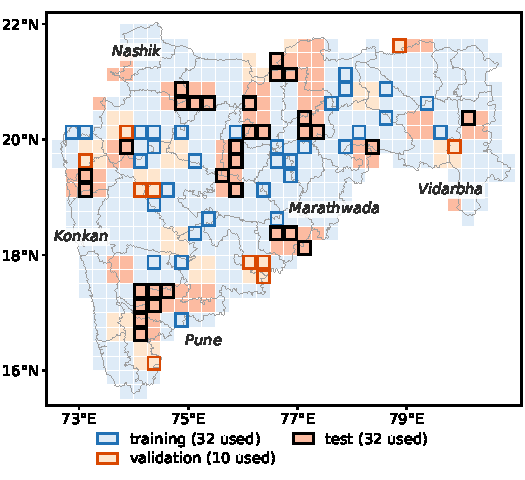
\includegraphics[width=\columnwidth]{fig_final_study_area.pdf}
\caption{Study grid over Maharashtra. Fill colour shows the super-block split and outlines mark the blocks used in the final experiment.}
\label{fig:area}
\end{figure}

\subsection{Sentinel-2 composites}
Sentinel-2 Level-2A scenes come from the Earth Search catalogue~\cite{earthsearch}. We keep scenes with cloud cover below 70\% and mask pixels that the Scene Classification Layer flags as no data, defective, cloud shadow, cloud, cirrus or snow. For each block and season we compute 14 dekadal composites of the per-pixel median NDTI, NDVI and four input bands over clear observations. Test blocks have cubes for 2018--2025 and training blocks for 2018--2022, and validation blocks are used for 2023 only.

\subsection{Land cover and weather}
Cropland is WorldCover 2021 class 40~\cite{worldcover}, resampled onto each cube's grid. Daily precipitation, 2\,m mean temperature and 0--7\,cm soil moisture at each block centre come from the Open-Meteo historical archive~\cite{openmeteo}, which serves ERA5-family reanalysis~\cite{era5}. Daily CHIRPS rainfall at 0.05$^\circ$~\cite{chirps}, obtained through SERVIR ClimateSERV~\cite{climateserv}, is averaged over each block's cell. Both series were complete for every block and day.

\subsection{Seasons, issue times and leads}
Season $Y$ runs from 11 September of year $Y$ to 31 January of year $Y{+}1$ (14 dekads). A forecast is issued at the end of dekad $t$, using the six composites up to and including $t$; issue dekads are those starting 1 November through 21 December, six per season. Each forecast predicts dekads $t{+}1$, $t{+}2$ and $t{+}3$ (leads $L=1,2,3$).

\section{Methods}
\subsection{Target and scoring mask}
For a pixel with SWIR reflectances $\rho_{11}$ and $\rho_{12}$ (Sentinel-2 bands B11 and B12) and red and narrow near-infrared reflectances $\rho_{4}$ and $\rho_{8A}$,
\begin{equation}
\mathrm{NDTI}=\frac{\rho_{11}-\rho_{12}}{\rho_{11}+\rho_{12}},\qquad
\mathrm{NDVI}=\frac{\rho_{8A}-\rho_{4}}{\rho_{8A}+\rho_{4}}.
\end{equation}
The target $y_{i,t+L}$ is the composite NDTI of pixel $i$ at dekad $t{+}L$. It is defined only if the pixel is WorldCover cropland, is clear at $t{+}L$, has $\mathrm{NDVI}_{i,t+L}<0.30$, and has at least one clear NDTI value in the six input dekads. The NDVI cutoff removes standing crops and rabi green-up, whose canopy water raises NDTI independently of residue~\cite{zheng}.

The forecast is therefore conditional on the pixel being clear and non-green at the target dekad. The condition was added to our protocol before any model of this study was trained (logged as a deviation on 14 October 2026, after NDTI was seen to follow crop greenness); it cannot be observed at issue time and also applies to training. It favours any model that can anticipate the harvest and penalises persistence (Section~\ref{sec:err}).

\subsection{Forecast units}
A forecast unit is one (block, season, issue, lead) combination. Of \finyNUnitsPossible{} possible test units, \finNUnitsCore{} contain a scored pixel (the \finxNUnitsEmpty{} empty units all target 1--10 December 2024, when no cropland pixel in those blocks passed the scoring mask). They hold \finNPixelForecasts{} pixel forecasts, and the scoring code asserts that every model and seed forecasts exactly the same pixels in every unit.

\subsection{Baselines}
\label{sec:baselines}
\emph{Persistence} carries forward the last clear input NDTI. \emph{Non-green persistence} carries forward the last clear input with NDVI below 0.30, falling back to persistence when there is none (\finxFallbackPersNG\% of forecasts). The \emph{six-dekad mean} averages the clear inputs. \emph{Seasonal persistence} uses the masked target at the same pixel and dekad in the previous season, falling back to persistence when it is missing (\finxFallbackSeas\% of forecasts; \finxFallbackSeasTwentyFour\% in 2024 and \finxFallbackSeasTwentyFive\% in 2025). \emph{Climatology} gives the per-pixel 10th, 50th and 90th percentiles (P10, P50, P90) of the masked target at the same dekad over the block's own 2018--2022 seasons, requiring at least \finxClimMinYears{} values; otherwise it uses block-wide, and as a last resort pooled training, quantiles for that dekad (together \finxFallbackClim\% of forecasts).

Climatology and seasonal persistence use only seasons before the test seasons, so they are temporally clean, but their access to each test location's own history gives them an advantage over the learned models. The first four baselines, like ridge, are point forecasts (P10\,=\,P50\,=\,P90).

\subsection{Ridge and the GBM}
Both models use the same per-pixel features, computed from dekads up to the issue dekad: the last clear NDTI and its age in dekads, the mean clear NDTI in the window, the change between the last two clear NDTI values, the last clear NDVI, the season-to-date maximum NDVI and the dekads since it, the issue dekad and the number of clear input dekads. The NDVI maximum and its timing reach back beyond the neural models' six-dekad window. Training rows are up to \finxPerUnitPx{} random scored pixels per block-season, issue and lead (\finNTrainRows{} training and \finNValRows{} validation rows). We call ridge and the GBM the feature-based models, and ConvLSTM and Earthformer the neural models. Ridge median-fills missing values, adds missing-value flags and a one-hot lead, and standardises the features; its penalty, chosen by validation MAE among values from 0.01 to 1000 in factors of ten, is the smallest of them (\finRidgeAlpha).

The GBM is scikit-learn's histogram gradient-boosting regressor~\cite{sklearn} with the quantile loss, one model per quantile level $\tau\in\{0.1,0.5,0.9\}$, with lead as a feature, \finxGbmLeaves{} leaves and at least \finxGbmMinLeaf{} samples per leaf. The learning rate was chosen from $\{$\finxGbmLRGrid$\}$, and the number of iterations, capped at \finxGbmCap, was set to the iteration at which the staged validation pinball loss was lowest. The selected learning rate is \finGbmLrFifty{} for all three quantiles, the lower edge of the grid, as was ridge's penalty.

\subsection{Weather variants}
We also trained GBM variants with block-level weather: \emph{+rain} adds ERA5 precipitation summed over the input window and over the issue dekad, \emph{+soil} and \emph{+temp} the issue-dekad mean soil moisture and temperature, \emph{+CHIRPS} CHIRPS sums over the windows of \emph{+rain}, and \emph{+all} all of them. Each variant re-selects only the iterations. Issue-dekad values from these retrospective products would not be available in real time.

\subsection{Neural models}
Each window is cut into \finxTilesPerWindow{} tiles of \finxPatch$\times$\finxPatch{} pixels; a sample is one tile at one issue time with a scored target (\finxNTrainSamples{} training and \finxNValSamples{} validation samples). For each input dekad the network receives NDTI, NDVI and four reflectances, forward-filled within the window, with a clear flag, the cropland mask and the dekad index. The head predicts P50 as the last forward-filled input NDTI plus a learned residual, and P10 and P90 as P50 minus and plus softplus offsets, so the quantiles cannot cross.

The ConvLSTM~\cite{convlstm} has three stacked cells with 64 hidden channels and 3$\times$3 kernels at full tile resolution (\finConvLSTMSeedOneParams{} parameters). Earthformer uses the official CuboidTransformerModel~\cite{earthformercode} (commit \finxEFCommit) with the SEVIR configuration (\finEarthformerSeedOneParams{} parameters); the only change is the initial downsampling, $[1,2,2]$ instead of $[3,2,2]$, so that a 128-pixel tile gives the same 32$\times$32 latent grid as a SEVIR frame (one token per 80\,m).

Both models minimise the masked pinball loss
\begin{equation}
\mathcal{L}=\frac{1}{3|M|}\sum_{i\in M}\sum_{\tau\in\{0.1,0.5,0.9\}}\max\left(\tau\,e_{i\tau},\,(\tau-1)\,e_{i\tau}\right),
\label{eq:pin}
\end{equation}
where $e_{i\tau}=y_i-\hat y_{i\tau}$ and $M$ is the set of scored pixels, with AdamW~\cite{adamw}, batch size \finxConvLSTMBS, linear warm-up and cosine decay to one-thousandth of the peak rate, flips and rotations, and gradient clipping. Every run trained for the full \finxEpochBudget{} epochs and was tested at the checkpoint with the lowest validation pinball loss. ConvLSTM uses a peak learning rate of \finyConvLSTMLR, weight decay \finyConvLSTMWD{} and \finxConvLSTMWarmup\% warm-up, set by hand. Earthformer uses a peak learning rate of \finyEarthformerLR, weight decay \finyEarthformerWD{} and \finxEarthformerWarmup\% warm-up; the learning rate is the SEVIR configuration's $10^{-3}$ at batch 32, scaled linearly~\cite{goyal}. Neither family was tuned further. The six reported runs took \finxNeuralTrainHours{} GPU hours on one 12\,GB \finxGPU, excluding the discarded run, with peak memory of at most \finxConvLSTMPeakGpuMax\,GB for ConvLSTM and \finxEarthformerPeakGpuMax\,GB for Earthformer.\footnote{Earthformer seed 341's memory record covers only its re-scoring, so its training peak is unknown.} Table~\ref{tab:seed} lists the per-seed training details.

\section{Experimental Design}
\subsection{Splits and metrics}
All fitted models are trained on 2018--2022 in the training blocks, selected on 2023 in the validation blocks and tested on 2024 and 2025 in the test blocks (\finxNTestBlockSeasons{} block-seasons), disjoint by super-block and by season. Hyper-parameters of the final runs were selected on validation data only.

For P50 we report the mean absolute error (MAE), root-mean-square error (RMSE) and bias (P50 minus target); for the quantile models (climatology, the GBM and its variants, and the neural models) also the pinball loss \eqref{eq:pin}, the 80\% interval coverage and the share of targets below P10. A point forecast has pinball loss equal to half its MAE, so point models are compared on MAE. Pooled metrics are pixel-weighted. In place of the protocol's MASE we report the ratio of pooled MAE to that of persistence.

\subsection{Statistical tests}
Pixels within a block are correlated and units overlap in time, so inference uses block metrics, which weight blocks equally. Comparisons use the \finNTestBlocks{} paired block differences: the win count (blocks in which the model has the lower error), a two-sided Wilcoxon signed-rank test~\cite{wilcoxon}, and a 95\% percentile bootstrap interval~\cite{efron} for the mean difference that resamples the \finNSuperblocks{} test super-blocks (2,000 draws). Percentage differences are relative to the reference model's mean block metric, unlike pooled percentages, which weight blocks by pixel count. Per-lead tests are judged against a Bonferroni threshold of 0.05/3; we report unadjusted $p$-values and say where the adjustment changes a conclusion.

\subsection{Seeds}
Each neural model was trained with seeds 340, 341 and 342. The aggregate for an architecture is the mean of the three per-seed metrics; the seed forecasts were never averaged into an ensemble. ConvLSTM seed 341 was resumed after an interruption, and Earthformer seed 341 was re-scored from its best checkpoint after a crash; neither is bit-for-bit reproducible.

\section{Results}
\subsection{Baselines and the GBM}
\label{sec:base}
Table~\ref{tab:main} gives pooled scores, and Fig.~\ref{fig:res} shows MAE by lead and block-level differences. Persistence has a strong upward bias ($\finPersBias$), because many of its forecasts carry a pre-harvest NDTI value into a non-green target. The six-dekad mean averages over more of the green period and is worse than persistence in every block. Non-green persistence is indistinguishable from persistence (\finPersNGVsPersWins{} wins, $p=\finPersNGVsPersP$). Seasonal persistence beats persistence in \finSeasVsPersWins{} of \finNTestBlocks{} blocks (MAE \finSeasMAE) but loses to climatology in all but \finSeasVsClimWins{} blocks ($p$\,\finSeasVsClimP). Because \finxFallbackSeas\% of its forecasts fall back to persistence, it is not a strong reference in this setting.

Climatology, the strongest training-free baseline, beats persistence in \finClimVsPersWins{} blocks and is nearly unbiased ($\finClimBias$), but its intervals are too narrow: only \finyClimCov{} of targets fall inside its 80\% interval and \finyClimBelow{} below its P10, as expected when per-pixel quantiles rest on only \finxClimMinYears{} to 5 seasons. Ridge (MAE \finRidgeMAE) beats persistence in all \finNTestBlocks{} blocks but not reliably climatology (\finRidgeVsClimWins{} wins, $p=\finRidgeVsClimP$).

The GBM has the lowest MAE of the feature-based models (\finGbmMAE) and is better than persistence and climatology in all \finNTestBlocks{} blocks, with mean block MAE differences of $\finGbmVsPersDiff$ (95\% CI \ci{\finGbmVsPersLo}{\finGbmVsPersHi}, Wilcoxon $p$\,\finGbmVsPersP) and $\finGbmVsClimDiff$ (\ci{\finGbmVsClimLo}{\finGbmVsClimHi}, $p$\,\finGbmVsClimP). Its pooled MAE is \finxGbmRelMAEVsPers\% below persistence (mostly from forecasts whose last clear input was green; Section~\ref{sec:err}) and \finxGbmRelMAEVsClim\% below climatology. Its pinball loss is lower than climatology's in every block, and its intervals cover \finyGbmCov{} of targets, with \finyGbmBelow{} below P10.

\begin{table*}[t]
\caption{Pooled test scores on the same \finNPixelForecasts{} pixel forecasts (\finNTestBlocks{} blocks, 2024 and 2025 seasons; NDTI units). Bias is P50 minus target. Ratio is pooled MAE divided by persistence MAE. Wins are blocks (of \finNTestBlocks) in which the model has the lower block MAE. Neural rows are means of the three per-seed metrics (not an ensemble forecast). Fallback is the share of forecasts that use a fallback rule.}
\label{tab:main}\centering\footnotesize\setlength{\tabcolsep}{5pt}
\begin{tabular}{lrrrrrrrrrr}\toprule
Model & MAE & RMSE & Bias & Pinball$^{a}$ & Cov.\ 80\% & Below P10 & Ratio & Fallback (\%) & Wins vs pers. & Wins vs clim.\\\midrule
Persistence & \finPersMAE & \finPersRMSE & $\finPersBias$ & \finPersPin & -- & -- & \finPersRelMAE & -- & -- & \finPersVsClimWins\\
Non-green persistence & \finPersNGMAE & \finPersNGRMSE & $\finPersNGBias$ & \finPersNGPin & -- & -- & \finPersNGRelMAE & \finxFallbackPersNG & \finPersNGVsPersWins & \finPersNGVsClimWins\\
Six-dekad mean & \finMovAvgMAE & \finMovAvgRMSE & $\finMovAvgBias$ & \finMovAvgPin & -- & -- & \finMovAvgRelMAE & -- & \finMovAvgVsPersWins & \finMovAvgVsClimWins\\
Seasonal persistence & \finSeasMAE & \finSeasRMSE & $\finSeasBias$ & \finSeasPin & -- & -- & \finSeasRelMAE & \finxFallbackSeas & \finSeasVsPersWins & \finSeasVsClimWins\\
Climatology & \finClimMAE & \finClimRMSE & $\finClimBias$ & \finClimPin & \finyClimCov & \finyClimBelow & \finClimRelMAE & \finxFallbackClim & \finClimVsPersWins & --\\
Ridge & \finRidgeMAE & \finRidgeRMSE & $\finRidgeBias$ & \finRidgePin & -- & -- & \finRidgeRelMAE & -- & \finRidgeVsPersWins & \finRidgeVsClimWins\\
GBM & \finGbmMAE & \finGbmRMSE & $\finGbmBias$ & \finGbmPin & \finyGbmCov & \finyGbmBelow & \finGbmRelMAE & -- & \finGbmVsPersWins & \finGbmVsClimWins\\
ConvLSTM & \finConvLSTMMAE & \finConvLSTMRMSE & $\finConvLSTMBias$ & \finConvLSTMPin & \finyConvLSTMCov & \finyConvLSTMBelow & \finConvLSTMRelMAE & -- & \finConvLSTMVsPersWins & \finConvLSTMVsClimWins\\
Earthformer & \finEarthformerMAE & \finEarthformerRMSE & $\finEarthformerBias$ & \finEarthformerPin & \finyEarthformerCov & \finyEarthformerBelow & \finEarthformerRelMAE & -- & \finEarthformerVsPersWins & \finEarthformerVsClimWins\\\bottomrule
\multicolumn{11}{l}{\scriptsize $^{a}$For point forecasts (rows without coverage) the pinball loss equals MAE/2 by construction; compare these rows on MAE and RMSE.}
\end{tabular}
\end{table*}

\begin{figure*}[t]
\centering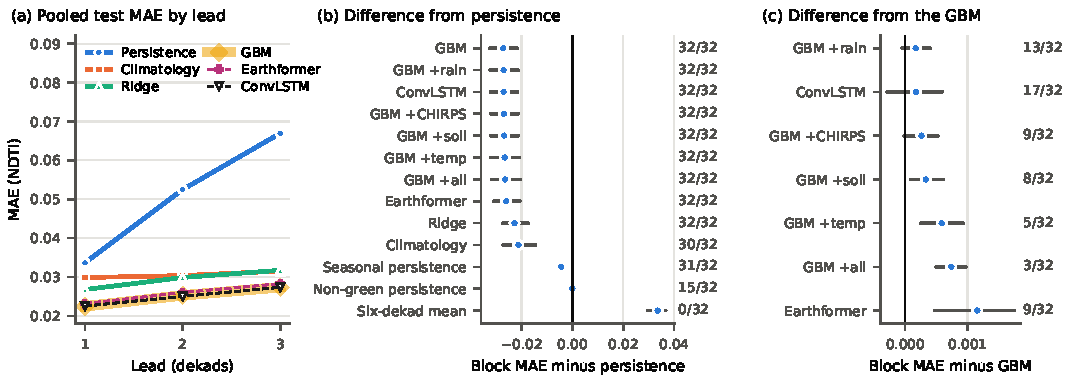
\includegraphics[width=\textwidth]{fig_final_results.pdf}
\caption{(a) Pooled test MAE by lead; the ConvLSTM line (thin, dashed, open markers) is drawn over the wide GBM line because the two nearly coincide. (b) Mean block MAE difference from persistence and (c) from the GBM, with 95\% super-block bootstrap intervals; numbers on the right are blocks (of \finNTestBlocks) in which the model has the lower MAE. Weather variants are labelled as in Table~\ref{tab:wx}. Neural models are means of the per-seed metrics.}
\label{fig:res}
\end{figure*}

\subsection{Neural models against the GBM}
Both neural models beat persistence in all \finNTestBlocks{} blocks and climatology in \finConvLSTMVsClimWins{} (ConvLSTM) and \finEarthformerVsClimWins{} (Earthformer) blocks. ConvLSTM and the GBM are statistically indistinguishable. On pooled pixels ConvLSTM is slightly lower, with an MAE of \finxConvLSTMMAEFive{} against \finxGbmMAEFive{} ($\finxPooledConvLSTMVsGbmMAERel$\%) and a pinball loss of \finxConvLSTMPinFive{} against \finxGbmPinFive{} ($\finxPooledConvLSTMVsGbmPinRel$\%). At the block level the mean difference has the opposite sign: ConvLSTM's mean block MAE is higher by $\finyConvLSTMVsGbmDiff$ (\ci{\finyConvLSTMVsGbmLo}{\finyConvLSTMVsGbmHi}, $p=\finConvLSTMVsGbmP$), although ConvLSTM has the lower MAE in \finConvLSTMVsGbmWins{} of \finNTestBlocks{} blocks; for the pinball loss $p=\finConvLSTMVsGbmPinP$. The views differ because pooled metrics weight blocks by pixel count.

Table~\ref{tab:seed} gives the results of each seed. The seed-to-seed standard deviation of ConvLSTM's pooled pinball loss (\finConvLSTMPinSd) is several times the pooled gap, and the seeds differ in sign against the GBM. Seed 340 has a higher block MAE, with a bootstrap interval above zero (\ci{\finxConvLSTMSeedOneVsGbmLo}{\finxConvLSTMSeedOneVsGbmHi}) although its Wilcoxon test is not significant; seed 341 has a lower block MAE and seed 342 is level with the GBM. We therefore treat the two models as tied on accuracy.

Earthformer is significantly worse than both. Its mean block MAE difference from the GBM is $\finyEarthformerVsGbmDiff$ (\ci{\finyEarthformerVsGbmLo}{\finyEarthformerVsGbmHi}, $p=\finEarthformerVsGbmP$), its pinball loss is also higher ($p$\,\finEarthformerVsGbmPinP), and against ConvLSTM it wins only \finEarthformerVsConvLSTMWins{} blocks ($p$\,\finEarthformerVsConvLSTMP). Each Earthformer seed is significantly worse than the GBM, and on validation data the best pinball loss of every ConvLSTM seed is lower than that of every Earthformer seed, so model selection and test give the same ranking. ConvLSTM's lower quantile is too high: \finyConvLSTMBelow{} of targets fall below its P10, and every seed is above the nominal 0.10. Earthformer's below-P10 share (\finyEarthformerBelow) is closer to the GBM's (\finyGbmBelow), but its coverage varies more across seeds than ConvLSTM's.

\begin{table*}[t]
\caption{Results and training details for each neural seed, with the GBM for reference (pooled test scores on the same pixel forecasts as Table~\ref{tab:main}). The $p$-value is the block-level Wilcoxon test against the GBM. Best epoch and validation pinball loss refer to the tested checkpoint; every run trained for \finxEpochBudget{} epochs.}
\label{tab:seed}\centering\footnotesize\setlength{\tabcolsep}{4.4pt}
\begin{tabular}{llrrrrrrrrrr}\toprule
Model & Seed & MAE & RMSE & Bias & Cov.\ 80\% & Below P10 & $p$ vs GBM & Best epoch & Val.\ pinball & Train (min) & Peak GPU (GB)\\\midrule
GBM & -- & \finxGbmMAEFive & \finGbmRMSE & $\finGbmBias$ & \finyGbmCov & \finyGbmBelow & -- & -- & -- & -- & --\\\midrule
ConvLSTM & 340 & \finxConvLSTMSeedOneMAEFive & \finxConvLSTMSeedOneRMSE & $\finxConvLSTMSeedOneBias$ & \finxConvLSTMSeedOneCov & \finxConvLSTMSeedOneBelow & \finxConvLSTMSeedOneVsGbmP & \finConvLSTMSeedOneBestEpoch & \finxConvLSTMSeedOneBestVal & \finConvLSTMSeedOneTrainMin & \finxConvLSTMSeedOnePeakGpuTrain\\
 & 341 & \finxConvLSTMSeedTwoMAEFive & \finxConvLSTMSeedTwoRMSE & $\finxConvLSTMSeedTwoBias$ & \finxConvLSTMSeedTwoCov & \finxConvLSTMSeedTwoBelow & \finxConvLSTMSeedTwoVsGbmP & \finConvLSTMSeedTwoBestEpoch & \finxConvLSTMSeedTwoBestVal & \finConvLSTMSeedTwoTrainMin & \finxConvLSTMSeedTwoPeakGpuTrain\\
 & 342 & \finxConvLSTMSeedThreeMAEFive & \finxConvLSTMSeedThreeRMSE & $\finxConvLSTMSeedThreeBias$ & \finxConvLSTMSeedThreeCov & \finxConvLSTMSeedThreeBelow & \finxConvLSTMSeedThreeVsGbmP & \finConvLSTMSeedThreeBestEpoch & \finxConvLSTMSeedThreeBestVal & \finConvLSTMSeedThreeTrainMin & \finxConvLSTMSeedThreePeakGpuTrain\\\midrule
Earthformer & 340 & \finxEarthformerSeedOneMAEFive & \finxEarthformerSeedOneRMSE & $\finxEarthformerSeedOneBias$ & \finxEarthformerSeedOneCov & \finxEarthformerSeedOneBelow & \finxEarthformerSeedOneVsGbmP & \finEarthformerSeedOneBestEpoch & \finxEarthformerSeedOneBestVal & \finEarthformerSeedOneTrainMin & \finxEarthformerSeedOnePeakGpuTrain\\
 & 341 & \finxEarthformerSeedTwoMAEFive & \finxEarthformerSeedTwoRMSE & $\finxEarthformerSeedTwoBias$ & \finxEarthformerSeedTwoCov & \finxEarthformerSeedTwoBelow & \finxEarthformerSeedTwoVsGbmP & \finEarthformerSeedTwoBestEpoch & \finxEarthformerSeedTwoBestVal & \finEarthformerSeedTwoTrainMin$^{a}$ & \finxEarthformerSeedTwoPeakGpuTrain$^{a}$\\
 & 342 & \finxEarthformerSeedThreeMAEFive & \finxEarthformerSeedThreeRMSE & $\finxEarthformerSeedThreeBias$ & \finxEarthformerSeedThreeCov & \finxEarthformerSeedThreeBelow & \finxEarthformerSeedThreeVsGbmP & \finEarthformerSeedThreeBestEpoch & \finxEarthformerSeedThreeBestVal & \finEarthformerSeedThreeTrainMin & \finxEarthformerSeedThreePeakGpuTrain\\\bottomrule
\multicolumn{12}{l}{\scriptsize $^{a}$Re-scored from its best checkpoint after a file-lock crash; the time includes the original training, and the peak memory of training was not recorded.}
\end{tabular}
\end{table*}

\subsection{Lead dependence, season and calibration}
Persistence error grows quickly with lead, climatology changes little and the GBM error grows slowly (Table~\ref{tab:lead}). Pooled over leads the GBM beats persistence in every block, and at lead 1 in \finxLeadOneGbmVsPersWins{} of \finNTestBlocks; its advantage over climatology shrinks with lead but is significant at every lead.

ConvLSTM and the GBM do not differ significantly at leads 2 and 3 ($p=\finxLeadTwoConvLSTMVsGbmP$ and \finxLeadThreeConvLSTMVsGbmP). At lead 1 the GBM is slightly ahead: ConvLSTM wins only \finxLeadOneConvLSTMVsGbmWins{} of \finNTestBlocks{} blocks, with an unadjusted $p$ of \finxLeadOneConvLSTMVsGbmP{}, which does not pass the Bonferroni threshold, and a bootstrap interval that includes zero (\ci{\finxLeadOneConvLSTMVsGbmLo}{\finxLeadOneConvLSTMVsGbmHi}). Earthformer is significantly worse than the GBM and than ConvLSTM at every lead, and all six of these $p$-values pass the adjusted threshold (largest \finxLeadOneEarthformerVsConvLSTMP).

Coverage is lower at lead 3 than at lead 1 for every quantile model, descriptively more so for the neural models than for the GBM. Errors were higher in 2024 than in 2025 for persistence (\finPersMAEYrTwentyFour{} against \finPersMAEYrTwentyFive), the GBM (\finGbmMAEYrTwentyFour{} against \finGbmMAEYrTwentyFive), ConvLSTM (\finConvLSTMMAEYrTwentyFour{} against \finConvLSTMMAEYrTwentyFive) and Earthformer (\finEarthformerMAEYrTwentyFour{} against \finEarthformerMAEYrTwentyFive), but not for climatology (\finClimMAEYrTwentyFour{} against \finClimMAEYrTwentyFive); no per-season test was run. ConvLSTM's 2024 coverage (\finxCovTwentyFourConvLSTM) was the lowest of the GBM and neural models.

\begin{table}[t]
\caption{Results by lead. Top: pooled MAE. Middle: block-level tests; percentages are relative to the reference's mean block MAE, negative values mean the GBM error is lower, wins are of \finNTestBlocks, and all GBM vs persistence and vs climatology $p$-values are \finxLeadOneGbmVsClimP. Bottom: 80\% interval coverage and share below P10.}
\label{tab:lead}\centering\footnotesize\setlength{\tabcolsep}{2.1pt}
\begin{tabular}{lrrr}\toprule
& Lead 1 & Lead 2 & Lead 3\\\midrule
Persistence MAE & \finPersMAELeadOne & \finPersMAELeadTwo & \finPersMAELeadThree\\
Climatology MAE & \finClimMAELeadOne & \finClimMAELeadTwo & \finClimMAELeadThree\\
GBM MAE & \finGbmMAELeadOne & \finGbmMAELeadTwo & \finGbmMAELeadThree\\
ConvLSTM MAE & \finConvLSTMMAELeadOne & \finConvLSTMMAELeadTwo & \finConvLSTMMAELeadThree\\
Earthformer MAE & \finEarthformerMAELeadOne & \finEarthformerMAELeadTwo & \finEarthformerMAELeadThree\\\midrule
GBM vs pers.\ (\%, wins) & $\finxLeadOneGbmVsPersRel$, \finxLeadOneGbmVsPersWins & $\finxLeadTwoGbmVsPersRel$, \finxLeadTwoGbmVsPersWins & $\finxLeadThreeGbmVsPersRel$, \finxLeadThreeGbmVsPersWins\\
GBM vs clim.\ (\%, wins) & $\finxLeadOneGbmVsClimRel$, \finxLeadOneGbmVsClimWins & $\finxLeadTwoGbmVsClimRel$, \finxLeadTwoGbmVsClimWins & $\finxLeadThreeGbmVsClimRel$, \finxLeadThreeGbmVsClimWins\\
ConvLSTM vs GBM ($p$) & \finxLeadOneConvLSTMVsGbmP & \finxLeadTwoConvLSTMVsGbmP & \finxLeadThreeConvLSTMVsGbmP\\
Earthformer vs GBM ($p$) & \finxLeadOneEarthformerVsGbmP & \finxLeadTwoEarthformerVsGbmP & \finxLeadThreeEarthformerVsGbmP\\
Earthformer vs ConvLSTM ($p$) & \finxLeadOneEarthformerVsConvLSTMP & \finxLeadTwoEarthformerVsConvLSTMP & \finxLeadThreeEarthformerVsConvLSTMP\\\midrule
Climatology cov.\ / below & \finxCovLeadOneClim{} / \finxBelowLeadOneClim & \finxCovLeadTwoClim{} / \finxBelowLeadTwoClim & \finxCovLeadThreeClim{} / \finxBelowLeadThreeClim\\
GBM cov.\ / below & \finxCovLeadOneGbm{} / \finxBelowLeadOneGbm & \finxCovLeadTwoGbm{} / \finxBelowLeadTwoGbm & \finxCovLeadThreeGbm{} / \finxBelowLeadThreeGbm\\
ConvLSTM cov.\ / below & \finxCovLeadOneConvLSTM{} / \finxBelowLeadOneConvLSTM & \finxCovLeadTwoConvLSTM{} / \finxBelowLeadTwoConvLSTM & \finxCovLeadThreeConvLSTM{} / \finxBelowLeadThreeConvLSTM\\
Earthformer cov.\ / below & \finxCovLeadOneEarthformer{} / \finxBelowLeadOneEarthformer & \finxCovLeadTwoEarthformer{} / \finxBelowLeadTwoEarthformer & \finxCovLeadThreeEarthformer{} / \finxBelowLeadThreeEarthformer\\\bottomrule
\end{tabular}
\end{table}

\subsection{Weather inputs}
No weather variant improved the GBM on the test set (Table~\ref{tab:wx}), and every variant has a higher pooled MAE. ERA5 rainfall made no detectable difference (\finGbmRainVsGbmWins{} wins, $p=\finGbmRainVsGbmP$); soil moisture ($p=\finGbmSoilVsGbmP$), CHIRPS rainfall ($p=\finGbmChirpsVsGbmP$), temperature ($p$\,\finGbmTempVsGbmP) and all variables together ($p$\,\finGbmAllVsGbmP) made the forecasts worse at the block level. Every variant's P50 model, and all but one of the variants' P10 and P90 models, reached its lowest validation loss at fewer iterations than the base model, which suggests that the weather columns let the trees fit season-specific patterns in the training years that did not carry over to the validation year.

\begin{table}[t]
\caption{Weather variants of the GBM. $\Delta$MAE is the mean block MAE difference from the base GBM (positive means worse); wins are blocks of \finNTestBlocks{} in which the variant is better. Iter.: selected iterations for P10/P50/P90.}
\label{tab:wx}\centering\footnotesize\setlength{\tabcolsep}{2.4pt}
\begin{tabular}{lrrrrrrr}\toprule
Variant & MAE & Pin. & Cov. & $\Delta$MAE & Wins & $p$ & Iter.\\\midrule
Base & \finGbmMAE & \finGbmPin & \finyGbmCov & -- & -- & -- & \finGbmItersTen/\finGbmItersFifty/\finGbmItersNinety\\
+rain & \finGbmRainMAE & \finGbmRainPin & \finyGbmRainCov & $\finGbmRainVsGbmDiff$ & \finGbmRainVsGbmWins & \finGbmRainVsGbmP & \finGbmRainItersTen/\finGbmRainItersFifty/\finGbmRainItersNinety\\
+soil & \finGbmSoilMAE & \finGbmSoilPin & \finyGbmSoilCov & $\finGbmSoilVsGbmDiff$ & \finGbmSoilVsGbmWins & \finGbmSoilVsGbmP & \finGbmSoilItersTen/\finGbmSoilItersFifty/\finGbmSoilItersNinety\\
+temp & \finGbmTempMAE & \finGbmTempPin & \finyGbmTempCov & $\finGbmTempVsGbmDiff$ & \finGbmTempVsGbmWins & \finGbmTempVsGbmP & \finGbmTempItersTen/\finGbmTempItersFifty/\finGbmTempItersNinety\\
+CHIRPS & \finGbmChirpsMAE & \finGbmChirpsPin & \finyGbmChirpsCov & $\finGbmChirpsVsGbmDiff$ & \finGbmChirpsVsGbmWins & \finGbmChirpsVsGbmP & \finGbmChirpsItersTen/\finGbmChirpsItersFifty/\finGbmChirpsItersNinety\\
+all & \finGbmAllMAE & \finGbmAllPin & \finyGbmAllCov & $\finGbmAllVsGbmDiff$ & \finGbmAllVsGbmWins & \finGbmAllVsGbmP & \finGbmAllItersTen/\finGbmAllItersFifty/\finGbmAllItersNinety\\\bottomrule
\end{tabular}
\end{table}

\subsection{Error by green-last share, cloudiness and region}
\label{sec:err}
In \finxGreenLastShare\% of scored forecasts the last clear input still had an NDVI of at least 0.30, so the field was green at issue and, by construction of the mask, non-green at the target. Split by pixel, \finyGreenGainShare\% of the GBM's pooled absolute-error reduction against persistence comes from these green-last forecasts. Across terciles of the units' green-last share (cuts at \finxGreenCutLo\% and \finxGreenCutHi\%; Table~\ref{tab:err}), persistence MAE rises from \finxPersMAEGreenOne{} to \finxPersMAEGreenThree, climatology varies little, and the GBM's reduction relative to persistence grows from \finxGbmGainGreenOne\% to \finxGbmGainGreenThree\%. The GBM still beats persistence and climatology in the least green tercile, and the neural models follow it closely in every tercile, Earthformer being the highest of the three. At the block level the GBM's absolute MAE gain over persistence is correlated with the green-last share (Spearman $\rho=\finRhoGainGreen$, $p=\finRhoPGainGreen$; shares from \finyRangeGreenLo\% to \finyRangeGreenHi\%).

Cloudiness explains little of the variation between blocks: clear-observation rates range from \finyRangeClearLo\% to \finyRangeClearHi\%, and neither persistence ($p=\finRhoPPersClear$) nor GBM error ($p=\finRhoPGbmClear$) is significantly related to them. Persistence error is higher in the least clear tercile of units (\finPersMAEClearLow{} against \finPersMAEClearHigh), plausibly because older last observations are more often pre-harvest, while GBM error barely changes. The clear-rate terciles and the block correlations were computed only for persistence, climatology and the GBM, not for the neural models.

By region (Table~\ref{tab:err}, MAE only, no tests), Marathwada has the highest pooled error for the GBM and both neural models, and Vidarbha the lowest among the four large divisions. Persistence error is well above climatology in every division except Konkan, most of all in Nashik. With \finyNBlocksKonkan{} to \finyNBlocksVidarbha{} test blocks per division, these figures are descriptive (Section~\ref{sec:region}).

\begin{table}[t]
\caption{Pooled MAE by green-last tercile and by division. Green: percentage of scored pixels whose last clear input was green (NDVI at least 0.30). Gain: GBM MAE reduction as a percentage of persistence MAE. ConvL.: ConvLSTM; Earthf.: Earthformer (means of seeds). $n$: test blocks.}
\label{tab:err}\centering\scriptsize\setlength{\tabcolsep}{1.9pt}
\begin{tabular}{lrrrrrrr}\toprule
Subset & Green & Pers. & Clim. & GBM & ConvL. & Earthf. & Gain\\\midrule
Tercile 1 & \finxGreenTercileShareOne & \finxPersMAEGreenOne & \finxClimMAEGreenOne & \finxGbmMAEGreenOne & \finxConvLSTMMAEGreenOne & \finxEarthformerMAEGreenOne & \finxGbmGainGreenOne\\
Tercile 2 & \finxGreenTercileShareTwo & \finxPersMAEGreenTwo & \finxClimMAEGreenTwo & \finxGbmMAEGreenTwo & \finxConvLSTMMAEGreenTwo & \finxEarthformerMAEGreenTwo & \finxGbmGainGreenTwo\\
Tercile 3 & \finxGreenTercileShareThree & \finxPersMAEGreenThree & \finxClimMAEGreenThree & \finxGbmMAEGreenThree & \finxConvLSTMMAEGreenThree & \finxEarthformerMAEGreenThree & \finxGbmGainGreenThree\\\midrule
Konkan ($n$=\finyNBlocksKonkan) & \finyGreenShareKonkan & \finPersMAEKonkan & \finClimMAEKonkan & \finGbmMAEKonkan & \finConvLSTMMAEKonkan & \finEarthformerMAEKonkan & \finyGbmGainKonkan\\
Marathwada ($n$=\finyNBlocksMarathwada) & \finyGreenShareMarathwada & \finPersMAEMarathwada & \finClimMAEMarathwada & \finGbmMAEMarathwada & \finConvLSTMMAEMarathwada & \finEarthformerMAEMarathwada & \finyGbmGainMarathwada\\
Nashik ($n$=\finyNBlocksNashik) & \finyGreenShareNashik & \finPersMAENashik & \finClimMAENashik & \finGbmMAENashik & \finConvLSTMMAENashik & \finEarthformerMAENashik & \finyGbmGainNashik\\
Pune ($n$=\finyNBlocksPune) & \finyGreenSharePune & \finPersMAEPune & \finClimMAEPune & \finGbmMAEPune & \finConvLSTMMAEPune & \finEarthformerMAEPune & \finyGbmGainPune\\
Vidarbha ($n$=\finyNBlocksVidarbha) & \finyGreenShareVidarbha & \finPersMAEVidarbha & \finClimMAEVidarbha & \finGbmMAEVidarbha & \finConvLSTMMAEVidarbha & \finEarthformerMAEVidarbha & \finyGbmGainVidarbha\\\bottomrule
\end{tabular}
\end{table}

\section{Discussion}
\subsection{Answer to the research question}
With both the test region and the test season held out, neither neural model forecast NDTI more accurately than the GBM. ConvLSTM was statistically tied with the GBM. Earthformer was worse than the GBM for every seed, and worse than both the GBM and ConvLSTM at every lead and in both test seasons. The GBM's improvement over persistence largely reflects the target definition; its improvement over climatology is the fairer measure of skill, and that comparison is conservative because climatology uses each test block's own history (Section~\ref{sec:baselines}).

\subsection{Why the GBM matches ConvLSTM}
\label{sec:tie}
The target's change over one to three dekads depends mostly on where the pixel stands in its own crop calendar, which the GBM features encode directly. Both families see the last clear observation and, directly or through the clear flags, its age, so both can learn the same harvest-timing correction to persistence. Our hypothesis for the tie is that spatial context adds little: most Indian holdings are small~\cite{agcensus} and neighbouring fields are harvested at different times, so neighbouring pixels probably say little about when a given field will be cleared. This would also fit the strength of tree ensembles on tabular problems~\cite{grinsztajn}. We did not test this hypothesis. A second explanation is equally open: the GBM sees season-to-date NDVI features beyond the neural models' window, so the comparison mixes information access with architecture.

\subsection{Possible reasons for Earthformer's higher error}
\label{sec:ef}
Several features of our setup may disadvantage Earthformer, and our experiments cannot separate them. Its \finEarthformerSeedOneParams{} parameters were trained on \finxNTrainSamples{} samples from \finxNTrainBlocks{} training blocks for \finxEpochBudget{} epochs, whereas its SEVIR configuration trains for 100 epochs~\cite{earthformercode}. Its best epochs (\finEarthformerSeedOneBestEpoch, \finEarthformerSeedTwoBestEpoch{} and \finEarthformerSeedThreeBestEpoch) came later than ConvLSTM's (\finConvLSTMSeedOneBestEpoch, \finConvLSTMSeedTwoBestEpoch{} and \finConvLSTMSeedThreeBestEpoch), and one seed peaked at epoch \finEarthformerSeedThreeBestEpoch{} of \finxEpochBudget. A longer schedule might help, but our runs cannot show this because the learning rate decays to one-thousandth of its peak within the budget. Its hyper-parameters were transferred from radar nowcasting without a search, and its stem gives one token per 80\,m, so several small fields can share a token.

\subsection{Why errors differ across regions}
\label{sec:region}
The regional pattern in Table~\ref{tab:err} follows the green-last share more than cloudiness. Vidarbha and Nashik have the largest green-last shares and GBM gains over persistence, Pune and Marathwada sit in the middle, and Konkan has the smallest share and the smallest gain, in line with the tested block-level correlation between gain and green-last share. Mean clear-observation rates in the four large divisions differ little (\finyClearRatePune\% to \finyClearRateVidarbha\%). Konkan, the clearest division (\finyClearRateKonkan\%), is the only one where persistence beats climatology, but it has only \finyNBlocksKonkan{} test blocks.

A plausible reading is that divisions with more fields still green at the November and December issue dates give persistence more pre-harvest values to carry forward. Cotton and pigeon pea are harvested after soybean and much of the rice~\cite{desharvest}, so a division's crop mix would shift its green-last share; without crop-type maps this remains an interpretation. Marathwada has a green-last share and clear rate close to Pune's, yet the highest error for the GBM, both neural models and climatology. Its high climatology error suggests that post-harvest NDTI there departs more from each pixel's earlier seasons, so the higher error probably reflects more variable conditions.

\subsection{Use for feedstock planning}
A forecast of this kind can tell a collection team which parts of a catchment are likely to show residue-like NDTI one to three dekads ahead. A planning system would also need the probability that a field is bare by a given dekad, and purchasable residue also depends on crop type, fodder use and burning, which NDTI does not observe. A conservative plan would rely on the lower quantile. The P10 of the GBM and that of Earthformer are close to nominal (\finyGbmBelow{} and \finyEarthformerBelow{} of targets below them, against a nominal 0.10), whereas ConvLSTM's is too high (\finyConvLSTMBelow), so a plan built on ConvLSTM's lower bound would overstate the lowest likely NDTI.

\subsection{Limitations}
\label{sec:lim}
Apart from the conditional target, the evaluation is limited in size: \finNTestBlocks{} blocks, each represented by one 12.8\,km window, and two seasons in the final evaluation. The training side is small too, with \finxNTrainBlocks{} training blocks, as many as the test set, and \finxNValBlocks{} validation blocks in one season, set by cube-building time; this probably limits the neural models, Earthformer most of all, more than the GBM. The regional figures rest on few blocks, \finyNBlocksKonkan{} in Konkan, and were not tested.

The comparison between families is not information-equal: the feature-based models train on up to \finxPerUnitPx{} pixels per unit but see season-to-date NDVI features, while the neural models see every scored pixel of a six-dekad window. Tuning was also unequal across families. WorldCover is fixed to 2021, issue-dekad weather is not available in real time, and the exact reanalysis product behind the Open-Meteo default endpoint was not recorded. NDTI is not residue mass and remains sensitive to soil moisture.

\section{Conclusion}
For one-to-three-dekad forecasts of NDTI on post-harvest cropland in Maharashtra, a GBM on per-pixel issue-time features was as accurate as ConvLSTM and more accurate than Earthformer. The GBM reached an MAE of \finGbmMAE{} against \finClimMAE{} for climatology, \finxGbmRelMAEVsClim\% lower, and was better than climatology in all \finNTestBlocks{} test blocks, while ConvLSTM was statistically tied with it ($p=\finConvLSTMVsGbmP$). Because the gain over persistence is concentrated in forecasts issued on still-green fields, the gain over climatology should guide use. A light model on open Sentinel-2 data could be used to rank parts of a catchment by expected NDTI, although we did not evaluate ranking skill and the index is not a tonnage.

A GBM restricted to the six-dekad window or neural models given the season-to-date features would separate information access from architecture, and a ConvLSTM with 1$\times$1 kernels would test whether spatial context helps. For operational use, the forecasts would also need a model of the probability that a field is bare by a given dekad and field calibration of NDTI against residue mass.

\section*{Use of AI Tools}
Generative AI tools were used for copy editing, LaTeX formatting, and routine code assistance. The authors designed the study, reviewed all outputs, and are responsible for the content.

\section*{Code and Data Availability}
The code and scripts that generate every number, table and figure are submitted with this report; the input data are open.

\section*{Author Contributions}
Abstract, Introduction (I), Study Area and Data (III), Methods (IV): H. Rathi. Related Work (II), Experimental Design (V): T. Wang. Results (VI), Discussion (VII), Conclusion (VIII): H. Rathi and T. Wang. H. Rathi built the data pipeline and ran the experiments. Time contributed: H. Rathi about 20 hours, T. Wang about 10 hours.

\begin{thebibliography}{99}
\bibitem{satat} Ministry of Petroleum and Natural Gas, Government of India, ``Sustainable Alternative Towards Affordable Transportation (SATAT),'' 2018. Accessed: Oct. 2026. [Online]. Available: \url{https://satat.co.in}
\bibitem{hiloidhari} M. Hiloidhari, D. Das, and D. C. Baruah, ``Bioenergy potential from crop residue biomass in India,'' \emph{Renew. Sustain. Energy Rev.}, vol. 32, pp. 504--512, 2014.
\bibitem{jain} N. Jain, A. Bhatia, and H. Pathak, ``Emission of air pollutants from crop residue burning in India,'' \emph{Aerosol Air Qual. Res.}, vol. 14, no. 1, pp. 422--430, 2014.
\bibitem{jethva} H. Jethva, O. Torres, R. D. Field, A. Lyapustin, R. Gautam, and V. Kayetha, ``Connecting crop productivity, residue fires, and air quality over northern India,'' \emph{Sci. Rep.}, vol. 9, Art. no. 16594, 2019.
\bibitem{desharvest} Directorate of Economics and Statistics, Ministry of Agriculture and Farmers Welfare, Government of India, ``Harvesting season of principal crops in major growing states,'' Appendix II, 2015. Accessed: Nov. 2026. [Online]. Available: \url{https://desagri.gov.in/wp-content/uploads/2021/04/Appendix2.pdf}
\bibitem{vandeventer} A. P. van Deventer, A. D. Ward, P. H. Gowda, and J. G. Lyon, ``Using Thematic Mapper data to identify contrasting soil plains and tillage practices,'' \emph{Photogramm. Eng. Remote Sens.}, vol. 63, no. 1, pp. 87--93, 1997.
\bibitem{quemada} M. Quemada and C. S. T. Daughtry, ``Spectral indices to improve crop residue cover estimation under varying moisture conditions,'' \emph{Remote Sens.}, vol. 8, no. 8, Art. no. 660, 2016.
\bibitem{zheng} B. Zheng, J. B. Campbell, G. Serbin, and J. M. Galbraith, ``Remote sensing of crop residue and tillage practices: Present capabilities and future prospects,'' \emph{Soil Tillage Res.}, vol. 138, pp. 26--34, 2014.
\bibitem{convlstm} X. Shi, Z. Chen, H. Wang, D.-Y. Yeung, W.-K. Wong, and W.-C. Woo, ``Convolutional LSTM network: A machine learning approach for precipitation nowcasting,'' in \emph{Proc. Adv. Neural Inf. Process. Syst.}, vol. 28, 2015, pp. 802--810.
\bibitem{earthformer} Z. Gao \emph{et al.}, ``Earthformer: Exploring space-time transformers for Earth system forecasting,'' in \emph{Proc. Adv. Neural Inf. Process. Syst.}, vol. 35, 2022, pp. 25390--25403.
\bibitem{earthformercode} Amazon Science, ``Earthformer: Official implementation,'' GitHub, 2022. Accessed: Nov. 2026. [Online]. Available: \url{https://github.com/amazon-science/earth-forecasting-transformer}
\bibitem{hively} W. D. Hively, B. T. Lamb, C. S. T. Daughtry, J. Shermeyer, G. W. McCarty, and M. Quemada, ``Mapping crop residue and tillage intensity using WorldView-3 satellite shortwave infrared residue indices,'' \emph{Remote Sens.}, vol. 10, no. 10, Art. no. 1657, 2018.
\bibitem{sentinel} M. Drusch \emph{et al.}, ``Sentinel-2: ESA's optical high-resolution mission for GMES operational services,'' \emph{Remote Sens. Environ.}, vol. 120, pp. 25--36, 2012.
\bibitem{sen2cor} M. Main-Knorn, B. Pflug, J. Louis, V. Debaecker, U. M\"{u}ller-Wilm, and F. Gascon, ``Sen2Cor for Sentinel-2,'' in \emph{Proc. SPIE}, vol. 10427, Image and Signal Processing for Remote Sensing XXIII, 2017, Art. no. 1042704.
\bibitem{timesat} P. J\"{o}nsson and L. Eklundh, ``TIMESAT: A program for analyzing time-series of satellite sensor data,'' \emph{Comput. Geosci.}, vol. 30, no. 8, pp. 833--845, 2004.
\bibitem{sakamoto} T. Sakamoto \emph{et al.}, ``A crop phenology detection method using time-series MODIS data,'' \emph{Remote Sens. Environ.}, vol. 96, no. 3--4, pp. 366--374, 2005.
\bibitem{greenearthnet} V. Benson \emph{et al.}, ``Multi-modal learning for geospatial vegetation forecasting,'' in \emph{Proc. IEEE/CVF Conf. Comput. Vis. Pattern Recognit.}, 2024, pp. 27788--27799.
\bibitem{predrnn} Y. Wang \emph{et al.}, ``PredRNN: A recurrent neural network for spatiotemporal predictive learning,'' \emph{IEEE Trans. Pattern Anal. Mach. Intell.}, vol. 45, no. 2, pp. 2208--2225, 2023.
\bibitem{simvp} Z. Gao, C. Tan, L. Wu, and S. Z. Li, ``SimVP: Simpler yet better video prediction,'' in \emph{Proc. IEEE/CVF Conf. Comput. Vis. Pattern Recognit.}, 2022, pp. 3170--3180.
\bibitem{tau} C. Tan \emph{et al.}, ``Temporal attention unit: Towards efficient spatiotemporal predictive learning,'' in \emph{Proc. IEEE/CVF Conf. Comput. Vis. Pattern Recognit.}, 2023, pp. 18770--18782.
\bibitem{earthnet} C. Requena-Mesa, V. Benson, M. Reichstein, J. Runge, and J. Denzler, ``EarthNet2021: A large-scale dataset and challenge for Earth surface forecasting as a guided video prediction task,'' in \emph{Proc. IEEE/CVF Conf. Comput. Vis. Pattern Recognit. Workshops}, 2021, pp. 1132--1142.
\bibitem{sevir} M. S. Veillette, S. Samsi, and C. J. Mattioli, ``SEVIR: A storm event imagery dataset for deep learning applications in radar and satellite meteorology,'' in \emph{Proc. Adv. Neural Inf. Process. Syst.}, vol. 33, 2020, pp. 22009--22019.
\bibitem{prithvi} D. Szwarcman \emph{et al.}, ``Prithvi-EO-2.0: A versatile multi-temporal foundation model for Earth observation applications,'' arXiv:2412.02732, 2024.
\bibitem{hyndman} R. J. Hyndman and A. B. Koehler, ``Another look at measures of forecast accuracy,'' \emph{Int. J. Forecast.}, vol. 22, no. 4, pp. 679--688, 2006.
\bibitem{lightgbm} G. Ke \emph{et al.}, ``LightGBM: A highly efficient gradient boosting decision tree,'' in \emph{Proc. Adv. Neural Inf. Process. Syst.}, vol. 30, 2017, pp. 3146--3154.
\bibitem{grinsztajn} L. Grinsztajn, E. Oyallon, and G. Varoquaux, ``Why do tree-based models still outperform deep learning on typical tabular data?'' in \emph{Proc. Adv. Neural Inf. Process. Syst.}, vol. 35, 2022, pp. 507--520.
\bibitem{quantile} R. Koenker and G. Bassett, Jr., ``Regression quantiles,'' \emph{Econometrica}, vol. 46, no. 1, pp. 33--50, 1978.
\bibitem{roberts} D. R. Roberts \emph{et al.}, ``Cross-validation strategies for data with temporal, spatial, hierarchical, or phylogenetic structure,'' \emph{Ecography}, vol. 40, no. 8, pp. 913--929, 2017.
\bibitem{indiamaps} udit-001, ``India maps data: GeoJSON state and district boundaries derived from the Census of India 2011 district maps,'' GitHub repository. Accessed: Nov. 2026. [Online]. Available: \url{https://github.com/udit-001/india-maps-data}
\bibitem{worldcover} D. Zanaga \emph{et al.}, ``ESA WorldCover 10 m 2021 v200,'' Zenodo, 2022, doi: 10.5281/zenodo.7254221.
\bibitem{earthsearch} Element 84, ``Earth Search STAC API,'' 2024. Accessed: Oct. 2026. [Online]. Available: \url{https://earth-search.aws.element84.com/v1}
\bibitem{openmeteo} Open-Meteo, ``Historical weather API,'' 2024. Accessed: Oct. 2026. [Online]. Available: \url{https://open-meteo.com/en/docs/historical-weather-api}
\bibitem{era5} H. Hersbach \emph{et al.}, ``The ERA5 global reanalysis,'' \emph{Q. J. R. Meteorol. Soc.}, vol. 146, no. 730, pp. 1999--2049, 2020.
\bibitem{chirps} C. Funk \emph{et al.}, ``The climate hazards infrared precipitation with stations: A new environmental record for monitoring extremes,'' \emph{Sci. Data}, vol. 2, Art. no. 150066, 2015.
\bibitem{climateserv} SERVIR, ``ClimateSERV,'' NASA and USAID, 2026. Accessed: Oct. 2026. [Online]. Available: \url{https://climateserv.servirglobal.net}
\bibitem{sklearn} F. Pedregosa \emph{et al.}, ``Scikit-learn: Machine learning in Python,'' \emph{J. Mach. Learn. Res.}, vol. 12, pp. 2825--2830, 2011.
\bibitem{adamw} I. Loshchilov and F. Hutter, ``Decoupled weight decay regularization,'' in \emph{Proc. Int. Conf. Learn. Represent.}, 2019.
\bibitem{goyal} P. Goyal \emph{et al.}, ``Accurate, large minibatch SGD: Training ImageNet in 1 hour,'' arXiv:1706.02677, 2017.
\bibitem{wilcoxon} F. Wilcoxon, ``Individual comparisons by ranking methods,'' \emph{Biometrics Bull.}, vol. 1, no. 6, pp. 80--83, 1945.
\bibitem{efron} B. Efron, ``Bootstrap methods: Another look at the jackknife,'' \emph{Ann. Statist.}, vol. 7, no. 1, pp. 1--26, 1979.
\bibitem{agcensus} Department of Agriculture, Cooperation and Farmers Welfare, Government of India, ``Agriculture Census 2015-16: All India report on number and area of operational holdings (provisional),'' New Delhi, India, 2018. Accessed: Nov. 2026. [Online]. Available: \url{https://agcensus.nic.in}
\end{thebibliography}
\end{document}
